
\documentclass[11pt,fancy,lang=es]{elegantbook}

\title{Apuntes Tel131 - Electrónica Digital}
\subtitle{Marie González-Inostroza}
\date{agosto, 2023}
\version{0.1.0}

%\author{Ethan Deng \& Liam Huang}
\institute{Universidad Técnica Federico Santa María}




\cover{portada.png}


\definecolor{customcolor}{RGB}{35, 100, 102}%
\definecolor{morado}{RGB}{189,13,207}
\colorlet{coverlinecolor}{customcolor}

\begin{document}

\maketitle

\frontmatter
\tableofcontents

\mainmatter


%\chapter*{Información general del curso}

\section{Descripción}
Las tecnologías de consumo, portables o de escritorio, como también las plantas industriales, requieren de electrónica digital para el manejo, procesamiento y transmisión de información. Pero el diseño y puesta a punto de esta electrónica digital implica el conocer una nueva forma de ver los circuitos y sistemas electrónicos: se conciben desde una óptica discreta y lógica según Boole. El curso “Sistemas Digitales” cubre los conceptos constitutivos del análisis y diseño de circuitos digitales y sistemas digitales en general, como también persigue la optimización de estos circuitos y hacer los diseños más eficientes, desde el punto de vista del hardware, del costo computacional y del costo económico.

Libro guía:\\
\textit{Digital Design and Computer Architecture} de David Harris y Sarah Harris. Capítulos 1 al 4.

 \section{Información de contacto}
 \subsection{Profesora}
\begin{itemize}
\item Marie González Inostroza
    \item E-mail: \email{marie.gonzalez@usm.cl}
  \item Horario de consultas: Lunes/jueves 13.00 a 14.00 presencial o en otros horarios online. En ambos casos, se debe agendar con anticipación.
\end{itemize}
\subsection{Ayudantes}
\begin{itemize}
    \item Catalina Ulloa 
        E-mail: \email{catalina.ulloa@sansano.usm.cl}
    \item Juan Pablo del Valle
E-mail: \email{juan.delvalle@sansano.usm.cl}
\end{itemize}

 \section{Horario}
\begin{itemize}
    \item Clase Martes: bloque 13-14 17:10 a 18:20 sala A014
  \item Clase Jueves: bloque 13-14 17:10 a 18:20 sala A015
  \item Ayudantía: por definir
\end{itemize}

 \section{Evaluaciones}
 
 Se realizarán 4 controles, un proyecto grupal y un examen final no eximible. 
 
La nota final ($NF$) será calculada de la siguiente forma:

\begin{equation}
     NF=P*0.3 + C*0.4 + E*0.3
\end{equation}

Donde $NE$ es la nota del examen, $NC$ es el promedio de los 3 mejores controles y $P$ es la nota del proyecto.\\

Se evaluará la realización de un examen recuperativo en caso de presentarse casos que lo ameriten.
%\chapter{Conceptos previos}
\section{Definición electrónica digital}
La electrónica digital es el campo en donde se estudian circuitos electrónicos que funcionan con lógica digital. Estos se basan en señales digitales que se interpretan en base a dos valores lógicos: 0 y 1. Estas son distintas a las señales analógicas, ya que usan rangos de valores, también se usa para manipulación de dígitos binarios con la función de administrar procesos y la implementación de sistemas electrónicos en los cuales la información esta codificada en dos estados, entregándole la capacidad de procesar y controlar varios sistemas y subsistemas.


\begin{figure}[hbt!]
  \centering
  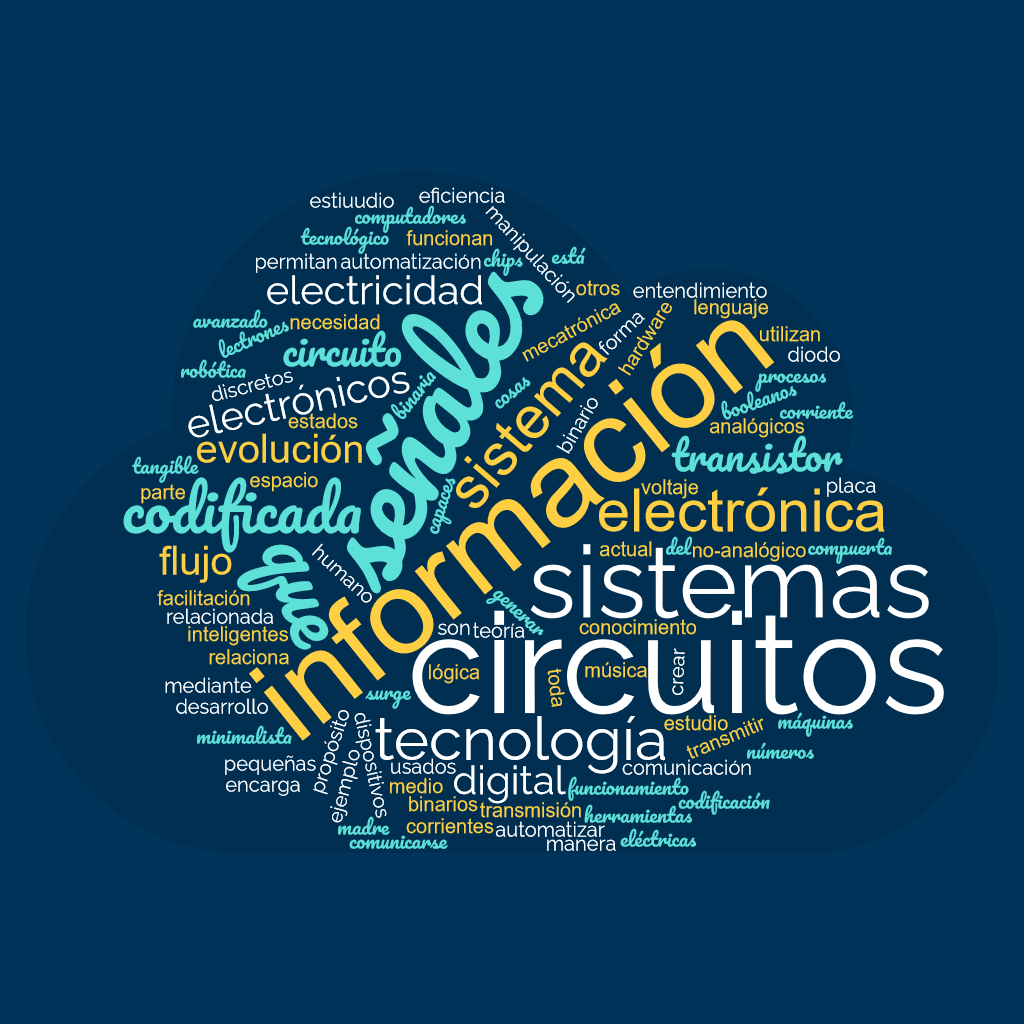
\includegraphics[width=\textwidth]{electronicadigital.png}
  \caption{Nube de palabras en base a los conceptos señalados para el término "Electrónica Digital"}
\end{figure}

\section{Componentes de los circuitos eléctricos} %Jose Acosta

\begin{itemize}
    \item Resistencia/Resistor:

Un resistor o resistencia es un componente electrónico que se opone al flujo de la corriente por este. Tienen dos terminales (entrada y salida) que no poseen polaridad, por lo tanto, no importa la orientación al momento de conectarlo.

\item Fuente de Voltaje:

Componente eléctrico que genera una diferencia de potencial (voltaje) de salida.

\item Fuente de corriente: Es un componente que proporciona corriente eléctrica al circuito.

\item Switch/interruptor:  dispositivo que permite abrir, cerrar o desviar un circuito eléctrico.
\end{itemize}

\section{Variables eléctricas}
Para el análisis de circuitos eléctricos  se debe conocer ciertos conceptos básicos que están directamente relacionado, Los cuales son:
\begin{itemize}
    \item Corriente Eléctrica: es un fenómeno físico causado por el desplazamiento de una carga, pudiendo ser flujo de electrones o de iones.
    
    \item Tensión Eléctrica: o diferencia de potencial es una magnitud física que indica la diferencia de potencial entre 2 de un circuito eléctrico.
    
    \item Potencia Eléctrica: Es la proporción de corriente eléctrica que transfiere un circuito eléctrico por unidad de tiempo, es decir, energía disipada durante un periodo de tiempo. se expresa en Watt[W]. Otra forma de representarlo es la cantidad de energía eléctrica transferida de una fuente de alimentación o generadora a un elemento consumido por unidad de tiempo
    
\end{itemize}

\section{Simbología circuitos} %Valeska Acuña

Hay una gran cantidad de componentes empleados en los diseños de circuitos, a continuación se presentarán la simbología de los elementos más comunes utilizados para esquematizar circuitos eléctricos.
Cabe destacar que elementos como las fuentes de corriente, fuentes de voltajes, resistencias, entre otros, tienen distintas representaciones, por lo que hay que considerar las existencias de estas para evitar confusiones.\\


\begin{circuitikz}

\draw (0,0) to[american voltage source, l=Fuente de Voltaje] ++(3,0)
(5,0) to[american controlled voltage source, l= Fuente de Voltaje Dependiente] ++(3,0) 
(10,0) to[american current source, l= Fuente de Corriente] ++(3,0);\\
\draw (0,-2) to[american controlled current source, l= Fuente de Corriente Dependiente] ++(3,0) 
(5,-2) to[battery, l = Batería] ++(3,0) 
(10,-2) to[battery1,l=Batería] ++(3,0);\\
\draw (0,-4) to[sinusoidal voltage source, l = Fuente Sinusoidal] ++(3,0) 
(5,-4) to[R,l=Resistencia] ++(3,0) 
(10,-4) to[european resistor, l= Resistencia] ++(3,0);\\
\draw (0,-6) to[capacitor, l=Capacitor] ++(3,0) 
(5,-6) to[inductor, l= Inductor] ++(3,0)
(10,-6) to[normal open switch, l= Switch] ++(3,0);\\
\draw (0,-8) to[empty diode, l=Diodo] ++(3,0) (5,-8) to[ammeter, l= Amperímetro] ++(3,0) (10,-8) to[voltmeter, l= Voltímetro] ++(3,0);\\
\draw (0,-10) to[empty led, l=LED] ++(3,0) %\node[ground, label=above:Tierra, scale = 2]() at (6.5,-9.5)  ++(3,0) 
%
%\node[npn, label=right:Transistor](npn) (11.5,-10) 
;
\end{circuitikz}

%Fin Valeska Acuña
Por otro lado, consideraremos que los cables cruzados no están conectados a menos que sea un cruce en T o con un punto:
 

\begin{circuitikz}

\draw (0,0) to ++(3,0) (3,0) to ++(0,3)
(4,0) to ++(3,0) (5.5,0) to ++(0,3) 
(8,1.5) to ++(3,0) (9.5,0) to ++(0,3) 
(12,1.5) to ++(3,0) (13.5,0)   to[short,-*]++(0,1.5) to ++(0,1.5) ;
\end{circuitikz}

\section{Definición cortocircuito, circuito abierto y cerrado}
%Inicio Javiera Alvarez
\begin{itemize}
    \item Circuito Cerrado: Un circuito se denomina cerrado cuando existe un camino cerrado, continuo; permitiendo que fluya la corriente eléctrica.
    \newline
    \item Cortocircuito:  circuito cerrado con una conexión directa entre dos terminales de un componente eléctrico. La corriente eléctrica toma el camino de menor resistencia, por lo que en un cortocircuito la corriente pasará por alto los caminos paralelos y viajará a través de la conexión directa.Esto provoca una corriente infinita, lo que probablemente derrita el aislamiento del cable y podría provocar un incendio u otros problemas asociados
    \newline
    \item Circuito abierto: corresponde a un circuito en que no fluye corriente ya que hay una discontinuidad de su camino. Cualquier circuito que no tenga un camino de retorno es un circuito abierto.
\end{itemize}

%\begin{figure}[hbt!]
%  \centering
%  \includegraphics[scale=0.3]{figure/circuitos.png}
%\end{figure}

\begin{figure}

             \centering
     
     
     \begin{subfigure}{0.3\textwidth}
             \centering
             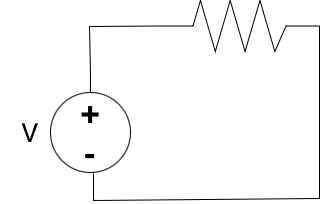
\includegraphics
[width=\textwidth]{images/C01/CircuitoCerrado.png}
         \caption{Circuito Cerrado}
         \label{fig:circCerrado}
     \end{subfigure}

     \begin{subfigure}{0.3\textwidth}
             \centering
             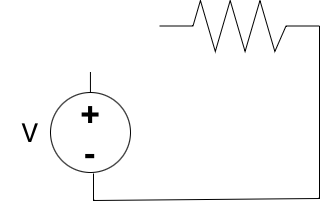
\includegraphics[width=\textwidth]{images/C01/C01-CircuitoAbierto.png}
         \caption{Circuito Abierto}
         \label{fig:circAbierto}
     \end{subfigure}
     

     \begin{subfigure}{0.3\textwidth}
             \centering
             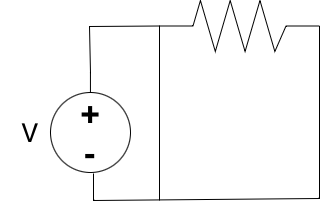
\includegraphics[width=\textwidth]{images/C01/CortoCircuito.png}
         \caption{Corto Circuito}
         \label{fig:CortoCirc}
     \end{subfigure}
     
     
     
     
     
        \caption{Ejemplos de condiciones de circuito}
        \label{fig:three graphs}
\end{figure}

    
    
    
    
        
%Fin Javiera Alvarez




%

\chapter{Análisis de circuitos lineales}

%INICIO ALEX ARAVENA %

\section{Partes de un circuito}
    
    \begin{itemize}
        \item \textbf{Nodo:} Un nodo es un punto de conexión entre dos o más componentes electrónicos. 

            \begin{figure}[h]
        \centering
        \begin{circuitikz}[american]
    \draw (0,0) 
    to[R=$R_1$] (3,0) node[label={[font=\footnotesize]above:A}] {}
    to[R=$R_2$] (6,0) ;
    \end{circuitikz}
        \caption{Ejemplo Nodo: En el punto A se unen las resistencias $R_1$ y $R_2$}
        \label{fig:ejNodo}
    \end{figure}
    \begin{center}

    
        \item \textbf{Rama:} Se forman al juntar dos nodos y los componentes entre ellos.\\\\
        
      
    
    \begin{figure}[h]
        \centering
        
    \begin{circuitikz}[american]
    \draw (0,0) 
    to[R=$R_1$] (3,0) node[label={[font=\footnotesize]above:A}] {}
    to[R=$R_2$] (6,0) node[label={[font=\footnotesize]above:B}] {}
    to[R=$R_3$] (9,0) ;
    \end{circuitikz}
        \caption{Ejemplo Rama: Existe una rama que involucra a los nodos A, B y la resistencia $R_2$.}
        \label{fig:ejRama}
    \end{figure}

  
   \item \textbf{Malla:} Definimos a la malla al conjunto de ramas que forman un camino cerrado, se requiere de mínimo dos ramas conectadas para formar una malla. Una malla es un circuito cerrado. \\
    
    Observe el siguiente ejemplo.
    \begin{center}
          
    \begin{circuitikz}[american]
    \draw (0,0) to[vsource, l=$V_1$, invert] (0,3) node[label={[font=\footnotesize]above:a}] {}
    to [R=$R_1$] (2,3) node[label={[font=\footnotesize]above:b}] {}
    to [R=$R_4$] (2,0) 
    (2,3) to [R=$R_2$] (4,3) node[label={[font=\footnotesize]above:c}] {}
    to (4,0)
    (4,3) to [R=$R_3$] (6,3)node[label={[font=\footnotesize]above:d}] {}
    to [R=$R_5$] (6,0) node[label={[font=\footnotesize]above:e}] {}
    to (0,0);
    \end{circuitikz}
    \end{center}
    
    En este ejemplo podemos plantear 3 mallas:
    \begin{enumerate}
        \item La de la fuente $V_1$ y las resistencias $R_1$ y $R_4$
        \item La de las resistencias $R_4$ y $R_2$
        \item La de las resistencias $R_3$ y $R_6$
        
    \end{enumerate}
    
    Las mallas no necesariamente deben ser de forma rectangular, por convención las vemos de esta forma, pero estas pueden tener una forma libre, únicamente se designa así por tener un orden y entendimiento simple.\\
    
    Pero en el caso que se muestra a continuación:
    

    \begin{center}
          
    \begin{circuitikz}[american]
    \draw (0,0) to[vsource, l=$V_1$, invert] (0,3) node[label={[font=\footnotesize]above:a}] {}
    to [R=$R_1$] (2,3) node[label={[font=\footnotesize]above:b}] {}
    to [R=$R_4$] (2,0) to (0,0)
    (2,3) to [R=$R_2$] (4,3) node[label={[font=\footnotesize]above:c}] {}
    
    ;
    \end{circuitikz}
    \end{center}
    
    Solo existe 1 malla que se forma en por la fuente y $R_1$ y $R_4$ puesto que la resistencia $R_2$ no lleva a ningún camino cerrado, por lo que deja un circuito abierto.

    \item \textbf{Lazo:} un lazo también es un conjunto de ramas que forman un camino cerrado, pero las mallas tienen la restricción de no contener ningún lazo dentro de otro. 

    \end{itemize}
    
    
    
%%%%%%%FIN ALEX ARAVENA%%%%%%%%%%%%%%%%%%%%%%%%%%%%%

%%%% INICIO DANIEL BARRIGA %%%%%
\section{Leyes circuitales básicas}






\subsection{Ley de Ohm}
Esta ley relaciona las variables de intensidad de corriente eléctrica, voltaje y resistencia eléctrica explicando así que cuando circula una corriente por un resistor se produce un voltaje a  través de los terminales, según la fórmula:\begin {equation*}
        V=R*I
        \label{fig:vir_ohm}
\end {equation*}

        Donde V:Voltaje[V]; I: Intensidad de corriente; R:Resistencia
 
    




\begin{example}[Ejemplo ley de Ohm en circuito con una resistencia]
\begin{center}

\begin{circuitikz}[american] 
\draw
        
	(3,-3) to (0,-3) to [V, l={V},i=$i_{t}$] (0,-6) 
   	(0,-6) to (3,-6) 
	(3,-3) to [R,i=$i_R$,l={$R$}] (3,-6) ;
        

\end{circuitikz}  
\end{center}

Basándonos en la figura, al tratarse de un circuito simple con una resistencia, los cálculos posibles son acotados a 3 (Suponiendo que se tiene 2 de los 3 valores necesarios en la ley de Ohm \emph{ V = I * R})\\
\begin{enumerate}
    \item Cálculo del Voltaje (Corriente por Resistencia) [V](Volt)
\begin {equation*}
    V = I * R
\end {equation*}

\item Cálculo  de la Corriente que pasa por la Resistencia (Voltaje divido por Resistencia) [A] (Ampere)
\begin {equation*}
    I = \frac{V}{R}
\end {equation*}


\item Cálculo de la Resistencia (Voltaje divido por Corriente) [Ω] (Ohm)
\begin {equation*}
    R = \frac{V}{I}
\end {equation*}\\
Además de la imagen podemos observar el convenio de los signos para la corriente, eso quiere decir que la corriente \emph{Sale} por el polo positivo de la fuente y \emph{Entra} por el polo negativo , lo coincide con el signo que esta tiene (para este caso positiva o con sentido horario)

Si asignamos los siguiente valores V= 5 [V] y R = 10[Ω]
El calculo de la corriente quedaria de la siguiente forma
\begin {equation*}
    I = \frac{5}{10} = 0.5 [A]
\end {equation*}

\end{enumerate}
\end{example}
%%%%FIN TOMAS CAMPUSANO%%%%
%%%%%% INICIO FRNCISCO CARDENAS %%%%%
\subsubsection{Equivalencia resistencia en serie y paralelo}

 
La resistencia equivalente es una forma de simplificar un circuito y facilitar el análisis de este. Una resistencia equivalente tendrá la misma caída de voltaje y la misma corriente que las que reemplaza para cierta posición.
\\

Para \textbf{resistencias en serie}, como las de la figura \ref{fig:rSerie}, la resistencia equivalente es la suma de cada resistencia, es decir, para \textit{n} resistencias en serie,
\begin {equation*}
    R_{eq} = R_1 + R_2 + ... + R_n
\end {equation*}\\

\begin{figure}[h]
     \centering
     \begin{subfigure}{0.35\textwidth}
        % \centering
         
    \resizebox{\textwidth}{!}{%
    \begin{circuitikz}[american]
    \draw (0,0) to[vsource, l=$V_0$, invert] (0,3)    
    to[R=$R_1$] (4,3)
    to[R=$R_2$] (4,0)
    to (0,0);
    \end{circuitikz}
    }%
         \caption{Resistencias en serie}
         
     \end{subfigure}\hspace{1em}
     \begin{subfigure}{0.35\textwidth}         
         
    \resizebox{\textwidth}{!}{%
    \begin{circuitikz}[american]
    \draw (0,0) to[vsource, l=$V_0$, invert] (0,3)
    to (1.5,3) -- (4,3)
    to[R=$R_1+R_2$] (4,0) -- (0,0);
    \end{circuitikz}
    }%
        \
         \caption{Resistencia equivalente}        
     \end{subfigure}
     
     
        \caption{Ejemplos de resistencia en serie y su equivalente}
        
        \label{fig:rSerie}
\end{figure}

\indent Para \textbf{resistencias en paralelo} se trabaja con la conductancia, \textit{G}, donde $G = \frac{1}{R}$. De este modo, la conductancia equivalente es la suma de cada conductancia particular, que se escribe en términos de las resistencias, ya que es el valor con el que se trabaja generalmente. Para \textit{n} resistencias en paralelo,
\begin {equation*}\label{eq:resispar2}
    \frac{1}{R_{eq}} = \frac{1}{R_1} + \frac{1}{R_2} + ... + \frac{1}{R_n}
\end {equation*}
\\

\begin{figure}[h]
     \centering
     \begin{subfigure}{0.35\textwidth}
        % \centering
         
    \resizebox{\textwidth}{!}{%
    \begin{circuitikz}[american]
    \draw (0,0) to[vsource, l=$V_0$, invert] (0,3)
    to(1.5,3)
    to(1.5,2.5)
    to[R=$R_1$] (1.5,0) -- (0,0)
    (1.5,3) to  (2,3) -- (4,3)
    to[R=$R_2$] (4,0)
    to[short, -*] (1.5,0);
    \end{circuitikz}    
    }%
         \caption{Resistencias en paralelo}
         
     \end{subfigure}\hspace{1em}
     \begin{subfigure}{0.35\textwidth}         
         
    \resizebox{\textwidth}{!}{%
    \begin{circuitikz}[american]
    \draw (0,0) to[vsource, l=$V_0$, invert] (0,3)
    to (1.5,3) -- (4,3)
    to[R=$R_{eq}$] (4,0) -- (0,0);
    \end{circuitikz}
    }%
        \
         \caption{Resistencia equivalente}        
     \end{subfigure}
     
     
        \caption{Ejemplos de resistencia en paralelo y su equivalente}
        
        \label{fig:rParalelo}
\end{figure}



    
En la figura \ref{fig:resiseq}a se puede ver un circuito simple con tres resistores, el cual puede ser simplificado como el circuito de \ref{fig:resiseqc} con un solo resistor. Además, de acuerdo a lo mencionado anteriormente, este resistor tiene una resistencia equivalente a la de los tres resistores del circuito original.

\begin{figure}[h]
     \centering
     \begin{subfigure}[b]{0.2\textwidth}
        % \centering
         \begin{circuitikz}[american]
    \draw (0,0) to[vsource, l=$V_0$, invert] (0,3)
    to[short, -*, i=$I_0$] (1.5,3)
    to[short, i>_=$I_1$] (1.5,2.5)
    to[R=$R_1$] (1.5,0) -- (0,0)
    (1.5,3) to [short, i=$I_2$] (2,3)
    to[R=$R_2$] (4,3)
    to[R=$R_3$] (4,0)
    to[short, -*] (1.5,0);
    \end{circuitikz}
         \caption{}
         \label{fig:resiseqa}
     \end{subfigure}
     
     
     \begin{subfigure}[b]{0.2\textwidth}
         %\centering
         
\begin{circuitikz}[american]
    \draw (0,0) to[vsource, l=$V_0$, invert] (0,3)
    to[short, -*, i=$I_0$] (1.5,3)
    to[short, i>_=$I_1$] (1.5,2.5)
    to[R=$R_1$] (1.5,0) -- (0,0)
    (1.5,3) to [short, i=$I_2$] (2,3) -- (4,3)
    to[R=$R_{eq^1}$] (4,0)
    to[short, -*] (1.5,0);
    \end{circuitikz}
         \caption{}
         \label{fig:resiseqb}
     \end{subfigure}
     
     
     \begin{subfigure}[b]{0.2\textwidth}
         %\centering
         
        \begin{circuitikz}[american]
    \draw (0,0) to[vsource, l=$V_0$, invert] (0,3)
    to[short, i=$I_0$] (1.5,3) -- (4,3)
    to[R=$R_{eq^2}$] (4,0) -- (0,0);
    \end{circuitikz}
         \caption{}
         \label{fig:resiseqc}
     \end{subfigure}
     
     
        \caption{Ejemplos de resistencia equivalente}
        
        \label{fig:resiseq}
\end{figure}
Como $R_2$ y $R_3$ están en paralelo, hacer una resistencia equivalente entre ellas:
\begin {equation*}
    R_{eq^1} = R_2 + R_3
\end {equation*}
Luego, $R_{eq^1}$ queda en paralelo con $R_1$, por lo que podemos formar un segundo equivalente:
\begin {equation*}\label{eq:resispar}
    \frac{1}{R_{eq^2}} = \frac{1}{R_1} + \frac{1}{R_{eq^1}}
\end {equation*}

\indent Finalmente la resistencia equivalente del circuito \ref{fig:resiseq}c queda expresada por,
\begin{equation*}
    R_{eq^2} = \frac{R_1(R_2 + R_3)}{R_1 + R_2 + R_3}
\end{equation*}
\\


\begin{remark}
   Para distinguir entre conexiones en serie y en paralelo, se puede tener en cuenta que en conexiones en serie, dos resistencias están unidas por un extremo cada una, mientras que en conexiones en paralelo, ambos extremos de dos resistencias están conectados mutuamente.
\end{remark}
 

\subsection{Potencia de una Resistencia}
La potencia eléctrica (\(P\)) en un circuito es una medida de la cantidad de energía transferida por unidad de tiempo. Esta potencia se puede calcular utilizando la ecuación fundamental \(P = I \cdot V\), donde \(I\) representa la corriente en amperios (\(A\)) y \(V\) es el voltaje en voltios (\(V\)). La potencia eléctrica se mide en watts (\(W\)) y representa la cantidad de energía que se transforma o consume en un circuito eléctrico en un intervalo de tiempo determinado. \\


 La potencia (\(P\)) en una resistencia (\(R\)) se puede calcular usando la ley de Ohm y la ley de Joule:

\begin{equation*}
P = I^2 \cdot R = \frac{V^2}{R}    
\end{equation*}


Donde:
\begin{align*}
    P &\text{ es la potencia en watts (W)} \\
    I &\text{ es la corriente en amperios (A)} \\
    V &\text{ es el voltaje en voltios (V)} \\
    R &\text{ es la resistencia en ohmios (\(\Omega\))}
\end{align*}

\begin{remark}
    En la práctica, parte de la potencia es disipada en forma de calor.
\end{remark}



\subsection{Leyes de Kirchoff}

Estas leyes, nombradas en honor al físico alemán Gustav Kirchhoff, permiten analizar y resolver circuitos complejos.

\subsubsection{Ley de Kirchhoff de Voltaje (LKV)}

La Ley de Kirchhoff de Voltaje establece que la suma algebraica de las caídas de tensión a lo largo de cualquier trayectoria cerrada en un circuito debe ser igual a cero. En otras palabras, si consideramos todas las caídas de tensión en los componentes a lo largo de un loop cerrado, la suma de estas tensiones debe anularse. Matemáticamente, se expresa como:

\begin {equation*}
    \sum_{k=1}^{n} V_k = V_1 + V_2 + V_3 + \ldots + V_n = 0
\end {equation*}

Donde \(V_k\) representa las caídas de tensión en los componentes individuales de la malla. 

          

\begin{example}[Ejemplo de aplicación de LKV]
%%%INICIO JESUS CHAFFE%%%
Se desea utilizar la ley de voltaje de Kirchhoff para analizar el siguiente circuito:

\centering{
 \begin{circuitikz}[american]

      %\draw[help lines] (0,0) grid (6,3);
       \draw (0,0) to [V, l={$V_\textrm{1}$}, invert] (0,3)
       to[R=$R_1$, v=$v_{R1}$] (3,3)
       to (6,3);
       \draw (6,3) to[R=$R_3$, v=$v_{R3}$] (6,0);
       \draw (0,0) to[short] (6,0);
       \draw (3,3) to[R=$R_2$, v=$v_{R2}$] (3,0);
       
    \end{circuitikz}
}

Primero tenemos que identificar los loop cerrados del circuito




\begin{circuitikz}[american voltages]
 \begin{scope}[local bounding box=circuit]
        \draw (0,0) to [V, l={$V_\textrm{1}$}, invert] (0,3)
       to[R=$R_1$, v=$v_{R1}$] (3,3)
       to (6,3);
       \draw (6,3) to[R=$R_3$, v=$v_{R3}$] (6,0);
       \draw (0,0) to[short] (6,0);
       \draw (3,3) to[R=$R_2$, v=$v_{R2}$] (3,0);
       \draw {(1.5,0.5) node {{\color{red}{$i_1$}}} (4.5,0.5) node {{\color{red}{$i_2$}}}};
       \draw[thick, red, <-, >=triangle 45] (1.8,0.8) arc (-60:240:0.8);
	  \draw[thick, red, <-, >=triangle 45] (4.8,0.8) arc (-60:240:0.8)
        ;
 \end{scope}        
 \draw[red,-stealth,rounded corners=1em] ([xshift=-1em]circuit.west) |-
 ([xshift=1em,yshift=1em]circuit.north east) -- 
 node[right,font=\sffamily]{$i_3$}
 ([xshift=1em]circuit.east);
\end{circuitikz}

Aplicando la ley de voltaje de Kirchhoff podemos obtener las ecuaciones de cada loop o circuito cerrado. 
\\

Para el loop de $i_1$ recorremos en el sentido de la corriente. Los componentes suman si van en el mismo sentido de la corriente (de más a menos) o restan si van en el sentido contrario (de menos a más):
\begin {equation*}
\notag -V_{1} + V_{R_1} + V_{R_2}  = 0
\end {equation*}


Para el loop de $i_2$ se tiene
\begin {equation*}
\notag V_{R_3} - V_{R_2} = 0
\end {equation*}

Para el loop de afuera, de $i_3$ tendremos:

\begin {equation*}
-V_1 + V_{R_1} + V_{R_3} =0
\end {equation*}

 Utilizando otras leyes podemos calcular otras variables del circuito.

 \begin{remark}
     La definición del sentido de las corrientes y de la polaridad de las resistencias es arbitrario al iniciar el análisis. 
 \end{remark}
\end{example}

\newpage
%INICIO DIEGO DE LA SOTTA
\subsubsection{Ley de Kirchoff de corriente (LKC)}
Esta ley establece que en cualquier nodo, la suma de las corrientes que \textbf{entran} es igual a la suma de las corrientes que \textbf{salen}. De forma equivalente, la suma de todas las corrientes que pasan por el nodo es igual a \textbf{cero}.
\begin{example}[Ejemplo de aplicación de LKC]
%%%INICIO JESUS CHAFFE%%%
Se desea utilizar la ley de corriente de Kirchhoff para analizar el siguiente circuito:

\centering{
 \begin{circuitikz}[american]

      %\draw[help lines] (0,0) grid (6,3);
       \draw (0,0) to [V, l={$V_\textrm{1}$}, invert] (0,3)
       to[R=$R_1$] (3,3)
       to (6,3);
       \draw (6,3) to[R=$R_3$] (6,0);
       \draw (0,0) to[short] (6,0);
       \draw (3,3) to[R=$R_2$] (3,0);
       
    \end{circuitikz}
}

Primero tenemos que identificar los nodos del circuito


\centering{
\begin{circuitikz}[american]

      %\draw[help lines] (0,0) grid (6,3);
       \draw (0,0) to [V, l={$V_\textrm{1}$}, invert, i_=$i_{V_1}$] (0,3) node[label={[font=\footnotesize]above:Nodo a}] {}
       to[R=$R_1$,*-*,i=$i_{R_1}$] (3,3) 
       to (6,3) node[label={[font=\footnotesize]above:Nodo b}] {};
       \draw (6,3) to[R=$R_3$,i=$i_{R_3}$] (6,0);
       \draw (0,0) to[short] (6,0);
       \draw (3,3) to[R=$R_2$,*-*,i=$i_{R_2}$] (3,0) node[label={[font=\footnotesize]below:Nodo c}] {};
       
    \end{circuitikz}}
    
En este caso, tenemos 3 nodos: Nodo a, Nodo b y Nodo c. Luego, para cada nodo, debemos analizar qué corrientes entran y cuáles salen.
\begin{itemize}
    \item Para el nodo a, la corriente de la fuente entra y la de la resistencia $R_1$ sale:
    \begin{equation*}
        i_{V_1}=i_{R_1}
    \end{equation*}

    \item Para el nodo b, la corriente de la resistencia $R_1$ entra y la de la $R_2$ y $R_3$ salen:
    \begin{equation*}
        i_{R_1}=i_{R_2}+i_{R_3}
    \end{equation*}

    \item Para el nodo c, la corriente de las resistencias $R_2$ y $R_3$entra y la de la fuente sale:
    \begin{equation*}
        i_{R_2}+i_{R_3}=i_{V_1}
    \end{equation*}
\end{itemize}
\end{example}
      
\iffalse
\begin{example}[Ejemplo de aplicación de LKC]
%%%INICIO JESUS CHAFFE%%%
Se desea utilizar la ley de corriente de Kirchhoff para analizar el siguiente circuito:

\centering{
 \begin{circuitikz}[american]

      %\draw[help lines] (0,0) grid (6,3);
       \draw (0,0) to [V, l={$V_\textrm{1}$}, invert] (0,3)
       to[R=$R_1$, v=$v_{R1}$] (3,3)
       to (6,3);
       \draw (6,3) to[R=$R_3$, v=$v_{R3}$] (6,0);
       \draw (0,0) to[short] (6,0);
       \draw (3,3) to[R=$R_2$, v=$v_{R2}$] (3,0);
       
    \end{circuitikz}
}

Primero tenemos que identificar los nodos del circuito: CAMBIO

\begin{circuitikz}[american]

      
       \draw (0,0) to [V, l={$V_\textrm{1}$}, invert] (0,3) 
       
       to[R=$R_1$, v=$v_{R1}$,*-*] (3,3)  node[label={[font=\footnotesize]above:$3$}] {}
       to (6,3);
       \draw (6,3) to[R=$R_3$, v=$v_{R3}$] (6,0);
       \draw (0,0) to[short] (6,0);
       \draw (3,3) to[R=$R_2$, v=$v_{R2}$] (3,0);
       \draw (3,6) node[label={above:$b$}] {} ;

    \end{circuitikz}

Aplicando la ley de voltaje de Kirchhoff podemos obtener las ecuaciones de cada loop o circuito cerrado. 
\\

Para el loop de $i_1$ recorremos en el sentido de la corriente. Los componentes suman si van en el mismo sentido de la corriente (de más a menos) o restan si van en el sentido contrario (de menos a más):
\begin {equation*}
\notag -V_{1} + V_{R_1} + V_{R_2}  = 0
\end {equation*}


Para el loop de $i_2$ se tiene
\begin {equation*}
\notag V_{R_3} - V_{R_2} = 0
\end {equation*}

Para el loop de afuera, de $i_3$ tendremos:

\begin {equation*}
-V_1 + V_{R_1} + V_{R_3} =0
\end {equation*}

 Utilizando otras leyes podemos calcular otras variables del circuito.

\end{example}
\fi

\iffalse
%%%% INICIO RICARDO DÍAZ%%%%%
\begin{example}[Ejemplo de aplicación de LKC]
\begin{center}
\begin{circuitikz}[american]
\draw

	(5,3) to (0,3) to [V, l={$V_\textrm{i}$},i=$i_{t}$] (0,6) 
   	(0,6) to (4,6) 
	(3,3) node[label={below:$a$}] {} to [R,i=$i_1$,l={$R_1$}] (3,6) node[label={above:$b$}] 
    (4,6) to(5,6)
    (5,3) to [R,i=$i_2$,l={$R_2$}] (5,6) ;

\end{circuitikz}
\end{center}
Debido a que se trata de un circuito en paralelo, el voltaje de $V_i$ se mantiene tanto en $R_1$ como en $R_2$, pero la corriente se divide en el nodo $a$, de tal forma que:

\begin {equation*}
i_{t} = i_1+ i_2 
\end {equation*}

Aplicando LKC, siendo: \[
\sum i=0
\]Se llega a:
\begin {equation*}
i_1+ i_2-i_{t}=0 
\end {equation*}

Ya que la ley de Kirchoff de corriente plantea que la corriente de salida es la misma que la de llegada, siendo el nodo $a$ donde se segmenta y en el nodo $b$ se vuelven a unir.
Aplicando la ley de Ohm, la ecuación queda:

\begin {equation*}
\frac{V_{1}}{R_1}+\frac{V_{2}}{R_2}-\frac {V_{i}} {R_t}=0
\end {equation*}
Siendo:
\begin {equation*}
R_t= \frac{R_1*R_2}{R_1+R_2}
\end {equation*}


\end{example}
\fi
\begin{remark}
    En este curso utilizamos la convención de que la polaridad va en el sentido de la corriente de + a - y que los componentes que suman son los que van en el mismo sentido de corriente. Existe la convención contraria, en que las fuentes suman y las resistencias restan.
\end{remark}

\section{Conexiones especiales de fuentes}
\subsection{Fuentes de Voltaje}


\subsubsection{Fuentes de voltaje en serie}



\begin{flushleft}
{Dada una configuración de $n$ fuentes de voltaje conectadas en serie, se define una fuente de voltaje equivalente como:}\\
\end{flushleft}


\begin{center}$
\displaystyle\sum_{i=1}^{n} V_i$
\end{center}


\begin{example}[Fuentes de voltaje en serie]
\begin{circuitikz}[american] 
        \draw
    (0,0) node[label={[font=\footnotesize]right:$a$}] {}
    to[V, l^=\mbox{$V_1$},invert,*-] (0,2) node[label={[font=\footnotesize]right:$b$}] {}
    to[V, l^=\mbox{$V_2$},invert,*-*] (0,4) node[label={[font=\footnotesize]right:$c$}] {}
    %to [short,-*] (0,5)
    
    ;
    \end{circuitikz}
    
En un circuito se tienen conectadas dos fuentes de voltaje en serie $V_1, V_2$ de valores. El voltaje de las fuentes se suma en cada nodo, por lo que, en el nodo b el voltaje será el voltaje en el nodo a $V_a$ más el de la fuente:
 

\begin{align*}
V_b&= V_a + V_1 \\
V_c&= V_b+V_2=V_a+V_1+V_2\\
\end{align*}

\end{example}


\begin{example}[Fuentes de voltaje en serie invertidas]
\begin{circuitikz}[american] 
        \draw
    (0,0) node[label={[font=\footnotesize]right:$a$}] {}
    to[V, l^=\mbox{$V_1$},invert,*-] (0,2) node[label={[font=\footnotesize]right:$b$}] {}
    to[V, l^=\mbox{$V_2$},*-*] (0,4) node[label={[font=\footnotesize]right:$c$}] {}
    %to [short,-*] (0,5)
    
    ;
    \end{circuitikz}
    
De forma similar al ejemplo anterior,debemos sumar los voltajes, sin embargo, la dirección de las fuentes hace que se resten:
 

\begin{align*}
V_b&= V_a + V_1 \\
V_c&= V_b-V_2=V_a+V_1-V_2\\
\end{align*}

\end{example}

\subsubsection{Fuentes de voltaje en paralelo}
\centering{
\begin{circuitikz}[american] 
        \draw
    (0,0) node[label={[font=\footnotesize]right:$a$}] {}
    to (0,1) to (1,1) to (1,1.5) to [V, l^=\mbox{$V_1$},invert] (1,2.5) to (1,3) to (0,3);
    \draw (0,1) to (-1,1) to (-1,1.5)to [V, l^=\mbox{$V_2$},invert] (-1,2.5) to(-1,3) to (0,3)  to (0,4) node[label={[font=\footnotesize]right:$c$}] {}
    ;
    \end{circuitikz}}

En caso de conectar n fuentes de voltaje en paralelo, podemos distinguir 2 casos:

    \begin{enumerate}
        \item {\textbf{Mismo voltaje:}}\\
       {Si las fuentes tienen el mismo valor de tensión, es equivalente a tener una única fuente con mayor capacidad de suministrar corriente.}\\
   
    \item {\textbf{Voltajes distintos:}}\\
    {Este caso rompe la Ley de Kirchoff de Voltaje, ya que se forma un circuito cerrado y no se cumple que la suma de voltajes sea 0.}
    \end{enumerate}
 


%%%%%%%%%%%%%%%%%Fin Rodrigo LOL%%%%%%%%%%%%%%%%%%%%%%%%
\subsection{Fuentes de Corriente}
%%%%%%%%%%%%%%%%%Inicio Rodrigo Lobos%%%%%%%%%%%%%%%%%%%

   
Las fuentes de corriente tienen su orientación definida (no así como las resistencias que le podemos dar una orientación para el cálculo de potencial y corriente), estas dan una fuente de corriente fija que pasa a través del circuito.\\




\subsection{Fuentes conectadas en paralelo}

\centering{
\begin{circuitikz}[american] 
        \draw
    (0,0) node[label={[font=\footnotesize]right:$a$}] {}
    to (0,1) to (1,1) to (1,1.5) to [I, l^=\mbox{$I_1$},invert] (1,2.5) to (1,3) to (0,3);
    \draw (0,1) to (-1,1) to (-1,1.5)to [I, l^=\mbox{$I_2$},invert] (-1,2.5) to(-1,3) to (0,3)  to (0,4) node[label={[font=\footnotesize]right:$c$}] {}
    ;
    \end{circuitikz}}
    
Al contrario del caso anterior, al conectar fuentes de corriente en paralelo sí se cumplen las leyes de Kirchoff. De hecho, lo que pasa es que se suman las corrientes, según LKC.


\begin{example}[Fuentes de coriente en paralelo]
¿Cuánta sería la corriente que pasa por el circuito?
\begin{center}
    \begin{circuitikz}[american] 
        
        \draw
    (0,0) to[I, l^=\mbox{$I_1$}] (0,3) -- (2,3)
      to[I, l^=\mbox{$I_2$}] (2,0) -- (0,0)
    (2,0) -- (4.5,0)
      to[I, l^=\mbox{$I_3$}] (4.5,3) -- (2,3)
    (4.5,3) -- (6.5,3)
      to[I,l^=\mbox{$I_4$}] (6.5,0) -- (4.5,0)
     (6.5,0) to [short,-](7,0)
     (7,0) to [short,-*](7,0)
     (6.5,3) to [short,-](7,3)
     (7,3) to [short,-*](7,3)
    ;
    \end{circuitikz}
    \begin{flushleft}

Tenemos 4 fuentes de corriente conectadas en paralelo, con valores de: $I_1 = 7[mA], I_2 =3[mA],I_3 =1[mA],I_4 =2[mA]$\\
Tendremos que definir las corrientes que apuntan hacia arriba como positivas, y las que apuntan hacia abajo como negativas:\\

\begin{center}
    $I_1 + I_3 - I_2 - I_4 =i_t$\\
    $7[mA] + 1[mA] - 3[mA] -2 [mA] = 3[mA]$\\
    $3[mA] = i_t$\\
\end{center}
\end{flushleft}
\end{center}
\end{example}



\subsubsection{Fuentes de corriente en serie}

\begin{circuitikz}[american] 
        \draw
    (0,0) node[label={[font=\footnotesize]right:$a$}] {}
    to[I, l^=\mbox{$I_1$},invert,*-] (0,2) node[label={[font=\footnotesize]right:$b$}] {}
    to[I, l^=\mbox{$I_2$},invert,*-*] (0,4) node[label={[font=\footnotesize]right:$c$}] {}
    %to [short,-*] (0,5)
    
    ;
    \end{circuitikz}
    

En este caso, debemos considerar cuáles son los valores de las fuentes. Si las fuentes tienen distinto valor, no se cumplirá la ley de Kirchoff de corriente, por lo que no se recomienda esta configuración con fuentes de distinto valor u orientación.

\iffalse
\begin{example}[Fuentes en serie]
\begin{center}
    \begin{circuitikz}[american] 
        \draw
    (0,0) to[I, l^=\mbox{$I_1$}] 
    (0,2) to[I, l^=\mbox{$I_2$}] (2,2) to [short,-*] (2.5,2)
    (0,0) -- (2,0) (2,0) to [short,-*] (2.5,0)
    ;
    \end{circuitikz}
    \begin{flushleft}
Tenemos un circuito donde se conecta una fuente de corriente $I1$ con un valor de $5[mA]$ con otra fuente $I_2$ de valor desconocido, sabiendo esto, ¿cuál debiese ser el valor de la fuente $I2$ para que este circuito sea posible?, ¿y si se añade una tercera fuente en serie, cuál debiese ser su valor?qué pasaría si conectamos esta tercera fuente en el sentido contrario a las otras?\\
Solución:\\
sabemos que al ser corrientes en serie, y tienen el mismo sentido en la corriente, podremos decir que tienen que ser iguales, y la corriente equivalente obtendrá el mismo valor:\\
\begin{center}
    $I_1 = I_2 =I_t$\\
    $5[mA] = I_2 = I_t$\\
\end{center}
Si se añadiese una tercera fuente, tendría que ocurrir lo mismo que en el caso anterior, si se llega a conectar al sentido contrario, podría dañar el circuito.
\end{flushleft}
\end{center}
\end{example}
\fi




\section{Casos especiales}
%% Inicio Antonia Figueroa %%
\begin{example}[Componente en un circuito abierto]
    \hspace{1.5cm}
    \begin{circuitikz}[american]
        \draw
            (0,6) to [R,l={$R_1$}] (3,6)
            (0,6) to [V, l={$V_\textrm{1}$}, i=$i_1$] (0,3) 
            (5,3) to (0,3) 
            (2.5,6) to [R,l={$R_2$},i=$i_2$](2.5,3)
            (2.5,6) node[label={above:$a$}] {} to [R,l={$R_3$}](5,6)
            (2.5,3) node[label={below:$b$}] {};
            
    \end{circuitikz}
    \hspace{2.0cm}
    \begin{circuitikz}[american]
        \draw
            (0,6) to [R,l={$R_1$}] (3,6)
            (2.5,6) to [R,l={$R_2$},i=$i_2$](2.5,3)
            (2.5,6) node[label={above:$Va$}] {} to [R,l={$R_3$}](5,6)
            (5,6) node[label={above:$Va$}] {}
            (2,3) to (2.5,3) node[label={below:$Vb$}] {} to (3,3)
            (3.6,6) node[label={below:$i=0$}] {};
    \end{circuitikz}
    
    
  
    Para este caso, se aprecia el nodo $a$ entre tres resistores, donde el $R_3$ es el particular ubicado en un extremo del circuito. ¿Qué implica esta condición?
    
        La primera Ley de Kirchhoff señala que las corrientes entrantes y salientes son las mismas. En este escenario, la corriente entrante es por el resistor $R_1$ y sale por $R_2$ y $R_3$; sin embargo, como la tercera resistencia no está conectada a ningún otro nodo, se intuye que la corriente sólo fluye por la resistencia $R_2$.

        Considerando lo anterior, se puede señalar que la corriente que atraviesa $R_3$ es de magnitud 0 ampere y que la diferencia de potencial entre antes y después del componente es 0.
    
\end{example}

\begin{example}[Componente omitido por cortocircuito]
    \hspace{1.5cm}
    \begin{circuitikz}[american]
        \draw
            (0,3) to [R,l={$R_1$}](0,6)
   	    (0,6) to (5,6) 
            (2.5,6) to [V, l={$V_\textrm{i}$},i=$i_1$] (2.5,3) 
            (5,6) node[label={above:$a$}]{} to [short,i=$i_1$] (5,3)
            (5,3) to (0,3) ;
    \end{circuitikz}
    \hspace{2.0cm}
    \begin{circuitikz}[american]
        \draw
   	    (2.5,6) to (5,6) 
            (2.5,6) to [V, l={$V_\textrm{i}$},i=$i_1$] (2.5,3) 
            (5,6) node[label={above:$a$}]{} to [short,i=$i_1$] (5,3)
            (5,3) to (2.5,3) ;
    \end{circuitikz}
    
  
        Para este escenario, hay dos caminos en paralelo a la fuente de voltaje, uno con un resistor y otro sin ningún componente.

        La Segunda Ley de Kirchhoff señala que, en una malla o subcircuito, la suma entre las caídas del voltaje suministrado por las fuentes de poder y el mismo voltaje suministrado es cero. 
        
        Considerando lo anterior y que en este caso se intuye que la corriente sólo va por el camino libre de resistencias, nunca hay caídas de voltaje, por lo que esta ley no se cumple en un cortocircuito.

        En la práctica, un cortocircuito es un malfuncionamiento del circuito en el que las resistencias son anuladas total o parcialmente, implicando que la intensidad del circuito en su totalidad es más de la que debiera soportar, llegando a provocar de chispazos a incendios de magnitudes variables.
\end{example}
%% Fin Antonia Figueroa %%
%% Diego Garrido Jofré %%

%\subsection{Análisis de corto circuito con leyes de kirchoff}
%Dado que la corriente puede fluir, sin oposición alguna, por un sistema o un componente en cortocircuito. Se pueden aplicar las leyes de Kirchhoff para analizar este comportamiento.


%Aplicando la Ley de Voltaje de Kirchhoff y teniendo en cuenta que un componente en cortocircuito no produce una baja en la tensión,  es decir no consume voltaje, se puede analizar el sistema considerando aquellos componentes que si interactúan con el voltaje y teniendo en consideración que la suma de voltajes del sistema, o de la malla a analizar, debe ser igual a cero.


%Lo mismo ocurre al aplicar la Ley de Corriente de Kirchhoff. Al tener un componente en cortocircuito, la diferencia de potencial entre un nodo a otro no va a variar,  entonces este no influirá en el paso de la corriente. De esta forma se puede analizar el circuito, sin tomar en cuenta al componente en cortocircuito y siguiendo la propuesta de que la suma de las corrientes en el sistema analizado, debe ser igual a 0.






\section{Métodos de análisis de circuitos}

\subsection{Método nodos}
\justify
El método de nodos nos permite encontrar la corriente y voltaje por cada resistencia en un circuito y consta de los siguientes pasos:
\begin{enumerate}
    \item Asignar tierra
    \item Nombrar nodos
    \item Resolver nodos fáciles 
    \item LKC + Ohm en nodos faltantes
    \item Resolver voltajes
	\item Aplicar Ohm para el resto
\end{enumerate}


\begin{example}[Método de Nodos]
Se busca determinar la corriente y voltaje del siguiente circuito:
\begin{center}        
    \begin{circuitikz}[american]
  %\draw[help lines] (0,0) grid (6,3);
  \draw (0,0) to[V=$V_1$,invert] (0,3)
   to[R=$R_1$] (3,3)
   to[R=$R_3$] (6,3);
   \draw (6,0) to[V=$V_2$,invert] (6,3);
   \draw (0,0) to[short] (6,0);
   \draw (3,0) to[R=$R_2$] (3,3);
   
    \end{circuitikz}
    \end{center}
Para esto, utilizaremos el método de los nodos.

\begin{enumerate}
    \item \textbf{Asignar tierra}: Se elige un nodo como referencia de tierra para simplificar el análisis. En este nodo, se asigna un voltaje igual a 0. En este caso, seleccionamos el nodo inferior.
    
    \begin{center}        
    \begin{circuitikz}[american]
  %\draw[help lines] (0,0) grid (6,3);
  \draw (0,0) to[V=$V_1$,invert] (0,3)
   to[R=$R_1$] (3,3)
   to[R=$R_3$] (6,3);
   \draw (6,0) to[V=$V_2$,invert] (6,3);
   \draw (0,0) to[short] (6,0);
   \draw (3,0) to[R=$R_2$] (3,3);
   \draw (3,0)to[short] node[ground] {GND} (3,-0.5)
   ;
    \end{circuitikz}
    \end{center}
    
    \item \textbf{Nombrar nodos}: Se asignan variables de voltaje a los nodos desconocidos. En este caso, nombramos el voltaje en el nodo superior izquierdo como \(V_{A}\), el nodo superior central como \(V_{B}\) y el nodo superior derecho como \(V_{C}\).

    \begin{center}        
    \begin{circuitikz}[american]
  %\draw[help lines] (0,0) grid (6,3);
  \draw (0,0) to[V=$V_1$,invert] (0,3) node[label={above:$V_A$}] {} 
   to[R=$R_1$] (3,3) node[label={above:$V_B$}] {} 
   to[R=$R_3$] (6,3);
   \draw (6,0) to[V=$V_2$,invert] (6,3) node[label={above:$V_C$}] {} ;
   \draw (0,0) to[short] (6,0);
   \draw (3,0) to[R=$R_2$] (3,3);
   \draw (3,0)to[short] node[ground] {GND} (3,-0.5)
   ;
    \end{circuitikz}
    \end{center}
    
    \item \textbf{Resolver nodos fáciles}: Si hay nodos con voltajes conocidos (por ejemplo, aquellos conectados a una fuente de voltaje), se pueden resolver directamente. En este caso, tendremos:
    \begin{align*}
        V_A=V_1
        V_C=V_2
    \end{align*} 
    
    \item \textbf{LKC + Ohm en nodos faltantes}: Aplicamos la Ley de Kirchhoff de Corrientes (LKC) en los nodos donde no conocemos el voltaje. Al hacerlo, también aplicamos la Ley de Ohm para representar las corrientes en función de los voltajes desconocidos.
    En este caso, el único nodo con voltaje desconocido es $V_B$ y partimos aplicando LKC en él:
    \newcommand{\iarronly}[1]{% name
 \node [currarrow, color=blue, anchor=center,
 rotate=\ctikzgetdirection{#1-Iarrow}] at (#1-Ipos) {};
 }

    \begin{center}        
    \begin{circuitikz}[american]
  %\draw[help lines] (0,0) grid (6,3);
  \draw (0,0) to[V=$V_1$,invert] (0,3) node[label={above:$V_A=V_1$}] {} 
   to[R=$R_1$,i=$i_{R_1}$, bipole current append style={color=blue}] (3,3) node[label={above:$V_B$}] {} 
   to[R=$R_3$,i>^=$i_{R_3}$, bipole current append style={color=blue}] (6,3);
   \draw (6,0) to[V=$V_2$,invert] (6,3) node[label={above:$V_C=V_2$}] {} ;
   \draw (0,0) to[short] (6,0);
   \draw (3,3) to[R=$R_2$,i>^=$i_{R_2}$, bipole current append style={color=blue}] (3,0);
   \draw (3,0)to[short] node[ground] {} (3,-0.5)
   ;
   
    \end{circuitikz}
    \end{center}

    Por LKC en el nodo B, tendremos
    \begin{align*}
        i_{R_1}&=i_{R_2}+i_{R_3}&&\\
        \frac{V_{R_1}}{R_1}&=\frac{V_{R_2}}{R_2}+\frac{V_{R_3}}{R_3}&& \text{por Ley de Ohm} \\
         \frac{V_1-V_B}{R_1}&=\frac{V_B}{R_2}+\frac{V_B-V_2}{R_3}&& \text{reemplazamos los voltajes para cada resistencia} \\         
    \end{align*}
    
    \item \textbf{Resolver voltajes}: Resolvemos el sistema de ecuaciones resultante de la LKC y las ecuaciones de Ohm para encontrar los voltajes desconocidos de los nodos.
    \begin{equation*}
        V_B=(\frac{1}{R_1}+\frac{1}{R_2}+\frac{1}{R_3})^{-1}\frac{V_1}{R_1}+\frac{V_2}{R_3}
    \end{equation*}
    
    \item \textbf{Aplicar Ohm para el resto de las corrientes y voltajes}: Utilizamos la Ley de Ohm para calcular las corrientes en los resistores y completar el análisis del circuito.
    En este caso, tendremos que para $R_1$:
    \begin{align*}
        V_{R_1}&=V_A-V_B\\
        i_{R_1}&=\frac{V_{R_1}}{R_1}
    \end{align*}

    Para $R_2$:
    \begin{align*}
        V_{R_2}&=V_B\\
        i_{R_2}&=\frac{V_{R_2}}{R_2}
    \end{align*}
    
    Para $R_3$:
    \begin{align*}
        V_{R_3}&=V_B-V_C\\
        i_{R_3}&=\frac{V_{R_3}}{R_3}
    \end{align*}
    Finalmente, bastaría con reemplazar con los valores ya calculados para tener el valor final.
\end{enumerate}



\end{example}

%%%%%%%%Eduardo Novoa%%%%%%%%%%%%%%
\subsection{Método mallas}
El método de mallas nos permite encontrar la corriente y voltaje por cada resistencia en un circuito y consta de los siguientes pasos:
\begin{enumerate}
    \item Identificar mallas
    \item Asignar corrientes de malla
    \item LKV + Ohm en mallas faltantes
    \item Resolver corrientes
	\item Aplicar Ohm para el resto
\end{enumerate}

\begin{example}[Método de Mallas]
Se busca determinar las corrientes y voltajes del siguiente circuito:

\begin{center}        
    \begin{circuitikz}[american]
  %\draw[help lines] (0,0) grid (6,3);
  \draw (0,0) to[V=$V_1$,invert] (0,3)
   to[R=$R_1$] (3,3)
   to[R=$R_3$] (6,3);
   \draw (6,0) to[V_=$V_2$,invert] (6,3);
   \draw (0,0) to[short] (6,0);
   \draw (3,0) to[R=$R_2$] (3,3);
   
    \end{circuitikz}
    \end{center}

Para resolver este circuito, utilizaremos el método de las mallas.

\begin{enumerate}
    \item \textbf{Identificar mallas}: Identificamos las mallas del circuito. En este caso, hay dos mallas.

    \begin{center}        
    \begin{circuitikz}[american]
  %\draw[help lines] (0,0) grid (6,3);
  \draw (0,0) to[V=$V_1$,invert] (0,3)
   to[R=$R_1$] (3,3)
   to[R=$R_3$] (6,3);
   \draw (6,0) to[V_=$V_2$,invert] (6,3);
   \draw (0,0) to[short] (6,0);
   \draw (3,0) to[R=$R_2$] (3,3);
   \draw [thick, <-] (2,1.5) arc(0:270:0.70);
       \draw (1.4,1.4) node {$i_1$};
       \draw [thick, <-] (5.4,1.5) arc(0:270:0.70);
       \draw (4.8,1.4) node {$i_2$};
    \end{circuitikz}
    \end{center}
    
    \item \textbf{Asignar corrientes de malla}: Asignamos variables de corriente a las mallas. Llamaremos \(i_1\) a la corriente de la malla izquierda y \(i_2\) a la corriente de la malla derecha.
    
    \item \textbf{LKV + Ohm en mallas faltantes}: Aplicamos la Ley de Kirchhoff de Voltajes (LKV) en las mallas donde no conocemos las corrientes. También aplicamos la Ley de Ohm para representar los voltajes en función de las corrientes de malla.\\
    \begin{center}        
    \begin{circuitikz}[american]
  %\draw[help lines] (0,0) grid (6,3);
  \draw (0,0) to[V=$V_1$,invert] (0,3)
   to[R=$R_1$] (3,3)
   to[R=$R_3$] (6,3);
   \draw (6,0) to[V_=$V_2$,invert] (6,3);
   \draw (0,0) to[short] (6,0);
   \draw (3,0) to[R=$R_2$] (3,3);
   \draw [thick, <-] (2,1.5) arc(0:270:0.70);
       \draw (1.4,1.4) node {$i_1$};
       \draw [thick, <-] (5.4,1.5) arc(0:270:0.70);
       \draw (4.8,1.4) node {$i_2$};
    \end{circuitikz}
    \end{center}
    Para la malla de $i_1$, recorremos en el sentido de las agujas del reloj, ya que la corriente fue definida en ese sentido, con lo que tendremos:
    \begin{equation*}
        V_{R_1}+V_{R_2}-V_1=0
    \end{equation*}
    Para la malla de $i_2$
    \begin{equation*}
        V_{R_3}+V_2-V_{R_3}=0
    \end{equation*}
    Reemplazamos con ley de Ohm
    \begin{align*}
        i_1R_1+(i_1-i_2)R_2-V_1&=0\\
        i_2R_3+V_2-(i_1-i_2)R_2&=0
    \end{align*}
    Con esto, obtenemos dos ecuaciones con dos incógnitas ($i_1$ e $i_2$).
    \item \textbf{Resolver corrientes}: Resolvemos el sistema de ecuaciones resultante de la LKV y las ecuaciones de Ohm para encontrar las corrientes de malla \(i_1\) y \(i_2\).
    \begin{align*}
        i_1&=\frac{R_2(V_1-V_2)+R_3V1}{R_1(R_2+R3)+R_2R_3}\\       
    i_2&=\frac{R_2(V_1-V_2)-R_1V_2}{R_1(R_2+R3)+R_2R_3}
    \end{align*}
    \item \textbf{Aplicar Ohm para el resto}: Utilizamos la Ley de Ohm para calcular las caídas de voltaje en los resistores y completar el análisis del circuito.
\end{enumerate}


\end{example}

\iffalse
\textbf{ \underline{Identifica las mallas: }}En este caso, el circuito llega a tener 2 mallas. Identificaremos 2 corrientes de lazo, denominados $i_1$ e $i_2$, las cuales son variables independientes. Aparte, ambos sentidos de los lazos van en sentido de las manecillas del reloj\\
\begin{figure}[h!]
    \begin{circuitikz}[american]
      %\draw[help lines] (0,0) grid (6,3);
      \draw (0,0) to[V=$V_A$,invert] (0,3)
       to[R=$R_1$, v<=$v_{R1}$] (3,3)
       to[R=$R_3$] (6,3);
       \draw (6,0) to[V_=$V_B$,invert] (6,3);
       \draw (0,0) to[short] (6,0);
       \draw (3,0) to[R=$R_2$] (3,3);
       \draw [thick, <-] (2,1.5) arc(0:270:0.70);
       \draw (1.4,1.4) node {$i_1$};
       \draw [thick, <-] (5.4,1.5) arc(0:270:0.70);
       \draw (4.8,1.4) node {$i_2$};
    \end{circuitikz}
  \end{figure}
Al definir una corriente de malla en cada malla, se tendra suficientes ecuaciones independientes para la resolucion del circuito.\\
\textbf{ \underline{Escribir la ley de voltaje (LVK) alrededor de cada malla:}}Al momento de escribir las ecuaciones LVK, se marca el esquema con los voltajes (+ y -) de cada elemento del circuito , usando la convención de signos para componentes pasivos.\\

\begin{figure}[h!]
    \begin{circuitikz}[american]
      %\draw[help lines] (0,0) grid (6,3);
      \draw (0,0) to[V=$V_A$, invert] (0,3)
       to[R=$R_1$, v=$v_{R1}$] (3,3)
       to[R=$R_3$, v=$v_{R3}$] (6,3);
       \draw (6,0) to[V_=$V_B$,invert] (6,3);
       \draw (0,0) to[short] (6,0);
       \draw (3,0) to[R=$R_2$, v=$v_{R2}$] (3,3);
       \draw [thick, <-] (2,1.5) arc(0:270:0.70);
       \draw (1.4,1.4) node {$i_1$};
       \draw [thick, <-] (5.4,1.5) arc(0:270:0.70);
       \draw (4.8,1.4) node {$i_2$};
    \end{circuitikz}
  \end{figure}
\\
\textbf{ \underline{Plantear sistema de ecuaciones:}} Escribimos una ecuacion para cada malla usando la ley de voltaje de Kirchoff(Suma de los voltajes alrededor de la malla e igualar dicha suma a cero). Se comienza con la esquina inferior izquierda , recorriendo la malla en el sentido de las agujas de reloj. El signo del voltaje dependera de donde entre a corriente (En este caso negativo).\\

\begin {equation*}
    -V_A + R_1 * I_1 + (R_1-R_2) * I_1 = 0
\end {equation*}
Aplicando la misma mecanica, con la segunda malla se comienza con la esquina inferior derecha, y debido a que la corriente entra por el lado positivo, este mismo determinara el signo del voltaje en la ecuacion. \\

\begin {equation*}
    V_B - (R_2 - R_1)*I_2 - R_3*I_2 = 0
\end {equation*}
\\
Ya mediante sistema de ecuaciones de las ecuaciones de las mallas, podemos obtener las corrientes que circulan en cada componente. 
%%%%%%%%Eduardo Novoa%%%%%%%%%%%

%Vicente Olmos%
\begin{example}[Método de nodos con fuente de voltaje]
\begin{circuitikz}[american]
\draw
	(8,4) to (0,4)
	to [V, l=\huge{$V_\textrm{s}$}, invert] (0,7) 
	
	(0,7) to [R, l=\huge{$R_1$}](4,7) to [R, l={\huge$R_3$}](8,7)
	(4,4) to [R, l=\huge{$R_2$}](4,7) 
	(8,4) to [R, l=\huge{$R_4$}] (8,7);

\end{circuitikz}

Se identifican los nodos, donde el nodo a tierra es de 0V



\begin{circuitikz}[american]
\draw
	(8,4) to (0,4)
	to [V, l=\huge{$V_\textrm{s}$}, invert] (0,7) 
	node[label={above:$a$}] {}
	(0,7) to [R, l={$R_1$}, *-*,v=$v_{R_1}$](4,7)  node[label={above:$b$}] {} to
	[R, l={$R_3$}, *-*,v=$v_{R_3}$] (8,7)
	(4,7) to [R, l={$R_2$}, *-*,v=$v_{R_2}$] (4,4) node[ground] {}
	(8,7) node[label={above:$c$}] {} to [R, l={$R_4$}, *-*,v=$v_{R_4}$] (8,4)  ;

\end{circuitikz}

Se puede obsevar como $V_a = V_s$ ya que tiene una fuente de voltaje asociada.

Se obtienen las ecuaciones de corriente mediante LCK para el nodo b:

\begin {equation*}
    I_{R_1}+I_{R_2}+I_{R_3} = 0
\end {equation*}

Se obtienen las ecuaciones de corriente mediante LCK para el nodo c:

\begin {equation*}
    -I_{R_3}= I_{R_4}
\end {equation*}

Se reemplaza por Ley de Ohm.

Nodo b:

\begin {equation*}
    \frac{V_b - V_s}{R_1}+\frac{V_b}{R_2}+\frac{V_b - V_c}{R_3}=0
\end {equation*}

Nodo c:

\begin {equation*}
    -\frac{V_c - V_b}{R_3}=\frac{V_c}{R_4}
\end {equation*}

Se puede ver como hay un signo menos en la corriente $I_R_3$ ya que hay que observar que las polaridades de la resistencia son distintas, en este caso la corriente esta entrando por el negativo, alterando el signo del nodo c para la corriente $I_R_3$.

Se puede despejar $V_b$ en las 2 ecuaciones:

\begin {equation*}
    V_b =\frac{\frac{V_s}{R_1}+\frac{V_c}{R_3}}{\frac{1}{R_1}+\frac{1}{R_2}+\frac{1}{R_3}}
\end {equation*}

\begin {equation*}
    V_b=R_3*V_c*(\frac{1}{R_3}+\frac{1}{R_4})
\end {equation*}

Para continuar con el analisis se asignaran valores numericos para hacer el proceso mas claro:

\hspace{2 cm}$V_s=12 V$\hspace{1 cm}$R_1=4\Omega$\hspace{1 cm}$R_2=2 \Omega$\hspace{1 cm}$R_3=6 \Omega$\hspace{1 cm}$R_4=10 \Omega$

Se reemplazan los valores dados:

\begin {equation*}
    V_b=\frac{\frac{12}{4}+\frac{V_c}{6}}{\frac{1}{4}+\frac{1}{2}+\frac{1}{6}}
\end {equation*}
\begin {equation*}
    V_b=6*V_c*(\frac{1}{6}+\frac{1}{10})
\end {equation*}

Calculando se obtiene:
\begin {equation*}
    V_b=3,27 +0,18V_c
\end {equation*}
\begin {equation*}
    V_b=1,6V_c
\end {equation*}

Se igualan las ecuaciones:
\begin {equation*}
    3,27+0,18V_c=1,6V_c
\end {equation*}

Y se obtiene el valor de $V_c=2,3V$

Con este resultado y la ecuacion 3.10 se calcula el valor de $V_b=3,68V$

Con todos los voltajes obtenidos se pueden determinar las corrientes:
\begin {equation*}
    I_{R_1}=\frac{V_b-V_s}{R_1}=\frac{3,68-12}{4}=-2,08 A
\end {equation*}
\begin {equation*}
    I_{R_2}=\frac{V_b}{R_2}=\frac{3,68}{2}= 1,84 A
\end {equation*}
\begin {equation*}
    I_{R_3}=\frac{V_b-V_c}{R_3}=\frac{3,68-2,3}{6}=0,23 A
\end {equation*}
\begin {equation*}
    I_{R_4}=\frac{V_c}{10}=\frac{2,3}{10}=0,23 A 
\end {equation*}

\end{example}
%Vicente Olmos%

\begin{example}[Método de malla con fuente de voltaje]
%%%%%%%%Sebastian Osses%%%%%%%%%%%%%%%%%%%%%%Sebastian Osses%%%%%%%%%%%%%%%%%%%%%%%%%%%%%%%%%%%%%%%%%%%%%%%%%%%%%%%%%%%%%%%%%%%%%%%%%%%%%%%%%%%%%%%%%%%%%

Resolveremos el siguiente circuito con el método de mallas  

\begin{circuitikz}[american]
\draw
	%(8,7) to
	(10,3) to (0,3) to [V, l=\huge{$V_\textrm{s}$}, invert] (0,7) 
   	(0,7) to [R, l=\huge{$R_1$},](3,7) to [R,l=\huge{$R_2$}](6,7)
	(6,3) to [R,l=\huge{$R_3$}](6,7)
    (6,7) to (10,7)
    (10,3) to [R,l=\huge{$R_4$}](10,7);

\end{circuitikz}
\\Donde:\\
\hspace{2 cm}$V_s=5 V$\hspace{1 cm}$R_1=8 \Omega$\hspace{1 cm}$R_2= 10 \Omega$\hspace{1 cm}$R_3= 20 \Omega$\hspace{1 cm}$R_4=15 \Omega$
\\\\
Comenzaremos la resolución identificando las mallas del circuito:
\\
\begin{circuitikz}[american]
\draw
	%(8,7) to
	(10,3) to (0,3) to [V, l=\huge{$V_\textrm{s}$}, invert] (0,7) 
   	(0,7) to [R, l=$R_1$,v=$V_{R_1}$](3,7) to [R,l=$R_2$,v=$V_{R_2}$](6,7)
	(6,7) to [R,l=$R_3$,v=$V_{R_3}$](6,3)
    (6,7) to (10,7)
    (10,7) to [R,l=$R_4$,v=$V_{R_4}$](10,3)
    {(3.1,5) node {\huge{\color{blue}{$i_1$}}} (7.9,5) node {\huge{\color{blue}{$i_2$}}}};
	\draw[very thick, blue, <-, >=triangle 45] (3.6,4.1) arc (-60:240:1);
	\draw[very thick, blue, <-, >=triangle 45] (8.4,4.1) arc (-60:240:1);
  %(0,7) to [R=$R_1$, *-*, v=$v_{R_1}$](4,7) node[label={above:$b$}] {} to [R=$R_3$, *-*, v=$v_{R_3}$](8,7)
\end{circuitikz}
\\\\
Notamos que tenemos 2 mallas: la de $i_1$ y la de $i_2$. Además, se observa que por $R_3$ circulan ambas corrientes y en sentido opuesto, por ende
\begin {equation*}
i_{R_3} = i_1- i_2 
\end {equation*}

Luego, por medio de la LKV obtendremos las ecuaciones de voltaje para cada malla. 
\\Para la malla de $i_1$ tenemos que en $V_s$ la corriente entre desde el negativo, mientras que por los resistores entra desde el lado positivo (convención de signo para elementos pasivos). Por lo tanto, tenemos:\\
\begin {equation*}
 -V_s + V_{R_1} + V_{R_2} + V_{R_3} = 0
\end {equation*}
Luego
\begin {equation*}
\notag V_s=V_{R_1}+V_{R_2}+V_{R_3}
\end {equation*} \\Para la malla de $i_2$ se tiene que en $R_4$ la corriente fluye desde el lado positivo, mientras que, en $R_3$ se considera la polaridad definida en la malla de $i_1$ en consecuencia, la corriente entra desde el lado negativo. Por lo tanto, se obtiene la siguiente relación:

\begin {equation*}
 -V_{R_3} + V_{R_4} = 0;
\end {equation*}
Expresión equivalente a 
\begin {equation*}
\notag V_{R_3}=V_{R_4}
\end {equation*} \\
Tras expresar las ecuaciones de LKV para cada malla, en ambas, reemplazaremos según la ley de Ohm los voltajes de cada resistor por el producto entre la corriente que circula por cada uno y sus respectivas resistencias. Además, que, para $V_{R_3}$ utilizaremos el valor de $i_{R_3}$ expresado arriba.\\\\
Malla de $i_1$:
\begin {equation*}
\notag V_s=R_1 i_1+R_2 i_1+R_3(i_1-i_2)
\end {equation*}\\
Malla de $i_2$: 
\begin {equation*}
\notag R_3(i_1-i_2)=R_4 i_2
\end {equation*}\\Reordenamos esta última y obtenemos la siguiente expresión para $i_2$
\begin {equation*}
i_2 = \frac{i_1 R_3}{R_3+R_4}
\end {equation*}\\Reemplazamos el valor de $i_2$ en la ecuación de la malla de $i_1$ se tiene
\begin {equation*}
\notag V_s= R_1 i_1+R_2 i_1+R_3 \left(i_1-\frac{i_1 R_3}{R_3+R_4} \right)
\end {equation*}\\
A continuación, reordenamos para obtener el valor algebraico de $i_1$:
\begin {equation*}
i_1=\frac{V_s}{R_1+R_2+R_3\left(1-\frac{R_3}{R_3+R_4}\right)}
\end {equation*}\\\\
 Ahora solo debemos reemplazar los valores de cada elemento del circuito para obtener  el valor de $i_1$ y a partir de este realizar el cálculo de los voltajes:

\begin {equation*}
\notag i_1=\frac{5}{8+10+20\left(1-\frac{20}{20+15}\right)}
\end {equation*}Calculando se obtiene:
\begin {equation*}
\notag i_1 = 0,188A = 188mA
\end {equation*}\\Luego, $i_2$ corresponde a:
\begin {equation*}
\notag i_2 = \frac{0,188 \cdot 20}{20+15}
\end {equation*}
Lo cual equivale a: 
\begin {equation*}
\notag i_2 = 0,107 A=107mA
\end {equation*}
Puesto que los valores de corriente calculados son positivos, las corrientes $i_1$ e $i_2$ fluyen en el mismo sentido que definimos.\\\\
Finalmente, tras haber calculado ambas corrientes, se calculan los valores de voltaje para cada resistor:
\begin {equation*}
\notag V_{R_1}=0,188\cdot8 = 1,504 V
\end {equation*}
\begin {equation*}
\notag V_{R_2} = 0,188 \cdot10 = 1,880 V
\end {equation*}
\begin {equation*}
\notag V_{R_3} = V_{R_4} = (0,188-0,107) \cdot 20 = 1,620 V
\end {equation*}


%%%%%%%%Sebastian Osses%%%%%%%%%%%%%%%%%%%%%%%%%%%%%%%%%%%%%%%%%%%%%%%%%%%%%%%%%%%%%%%%%%%%%%%%%%%%%%%%%%%%%%%%%%%%%%%%%%%%%%%%%%%%%%%%


\end{example}

%%%%%%%%%%%%%% INICIO LEO PONCE %%%%%%%%%%%%%%%%55
\newpage
\begin{example}[Método de Mallas con 2 fuentes de voltaje invertidas]
\\


Una malla es cualquier trayectoria cerrada de un circuito.

Para resolver algún ejercicio por método de mallas, es importante tener en cuenta que se trabajan con las leyes de Ohm y Kirchhoff. Puede ser tanto la ley de corriente, como ley de voltaje de Kirchhoff.
\iffalse
\begin{figure}[H]
    \centering
  \begin{subfigure}{\textwidth}
    \includegraphics[scale= 0.35]{SinFuenteinvertida.PNG}
    \caption{Ejemplo a resolver sin invertir una fuente}
    \label{fig:Imagen1}
  \end{subfigure}
  
  \begin{subfigure}{\textwidth}
    \includegraphics[scale=0.35]{ConFuenteinvertida.PNG}
    \caption{Ejemplo a resolver con una fuente invertida}
    \label{fig:Imagen2}
  \end{subfigure}
  
\end{figure}
\fi
En esta entrega se resolverán los circuitos de la figura 3.10 y 3.11, donde se tendrá que obtener el voltaje que hay entre la resistencia 1 y 2 (Vo). El objetivo de resolver estos dos circuitos, teniendo uno de ellos con una fuente invertida, es poder evaluar como se comporta el voltaje en una zona cuando se invierte una fuente.


Para los ejemplos a resolver, se ocupará la ley de voltaje de Kirchhoff, la cual dice que “La suma de los voltajes en una malla es igual a cero”.

\begin {equation*}
\notag
\displaystyle\sum_{n=1}^{} V_n=0
\end {equation*}
\begin{center}
Donde n es el numero de voltajes de los componentes en la malla.
\end{center}
\\
Pasos por seguir:
\begin{enumerate}
    \item Identificar las mallas y sentido de la corriente en aquellas mallas.
    \item Aplicar método de mallas con voltaje de Kirchhoff.
    \item Resolver ecuaciones de respectivas mallas.
    \item Encontrar términos de corrientes y/o voltaje.

\end{enumerate}

\newpage
\textbf{Ejemplo figura 1a (Sin invertir fuentes):}

\iffalse
\begin{figure}[H]
    \centering
    \includegraphics[scale = 0.4]{image/SinFuenteinvertida1.png}
    \caption{Circuito sin invertir fuentes y con sentido de corriente antihorario}
    \label{fig:1011101011}
\end{figure}
\fi
Siguiendo los pasos propuestos, identificamos que el circuito solo tiene una malla, por lo tanto, tendremos una ecuación de malla. Por consiguiente, utilizamos el método de mallas de voltaje(V=IR).
\\
Trazaremos el sentido de la corriente del circuito en antihorario (Opuesto a las manecillas del reloj), ese será el flujo de la corriente. Partimos en la fuente de voltaje V1, entrando por la parte negativa y saliendo por la positiva, por convención de signos, y puesto que no hay caída de voltaje, el signo que tomará esa fuente es negativo. Para el caso de las resistencias, utilizamos la ley de ohm para complementar con la ecuación de voltaje de Kirchhoff, puesto que el voltaje se expresa como la multiplicación de la corriente que pasa por la resistencia, por la resistencia. Al tener dos resistencias incluimos aquellas en la ecuación.
\\
Por último, nos encontramos con la segunda fuente V2, donde el flujo de corriente que pasa por ella va de positivo a negativo, por lo tanto, su signo es positivo puesto que cae voltaje. Como no tenemos más elementos en nuestro circuito y siguiendo la ley de Kirchhoff, la suma de voltajes es igual a cero, por ende, igualamos nuestra ecuación (3.43) a cero.
\begin{center}
\begin {equation*}
-V1+R1*I+R2*I+V2=0
\end {equation*}
\end{center}

Para hallar la corriente que pasa por la resistencia R1, debemos despejar de la ecuación (1) la corriente I. 


\begin {equation*}
\notag
-V1+R1*I+R2*I+V2=0
\longrightarrow
2000*I+1=0
\longrightarrow
I= \frac{-1}{2000}
\longrightarrow
I=-0,0005[A]
\end {equation*}

Como la corriente I, de valor -0,0005[A], pasa por la resistencia R1,se debe obtener el valor de voltaje que cae en esa resistencia. Puesto que el voltaje Vo que queremos encontrar es lo mismo que el voltaje en el nodo b, se hace una diferencia de voltaje entre los nodos a y b, para hallar el valor de b (Vb=Vo).
\begin{center}
\begin {equation*}
Vab=Va-Vb
\end {equation*}
\end{center}

Puesto que se conoce el valor de la corriente en la resistencia R1, se ocupa ley de ohm para hayar el voltaje que cae en dicha resistencia.

\begin {equation*}
\notag
VR1= R1*I
\longrightarrow
VR1=1000*-0,0005
\longrightarrow
VR1= -0,5[V]
\end {equation*}

\newpage
Puesto que el voltaje que cae en la resistencia R1, esta entre los nodos a y b, se obtuvo el valor de Vab a travez de la ecuación(3.44).Ahora bien, el valor Va se puede deducir del sistema, puesto que en el nodo a, el único valor de voltaje que pasa por él, es el de la fuente V1.

Teniendo los dos valores de volatje (Vab y Va), se hace un despeje en la ecuación (3.44), para hayar el valor de Vb (Que es igual a Vo)

\begin {equation*}
\notag
Vab= Va-Vb
\longrightarrow
-0,5=5-Vb
\longrightarrow
-5,5=-Vb
\longrightarrow
5,5=Vb
\end {equation*}

El valor de voltaje que pasa entre la resistencia 1 y 2 (Nodo b) es 5,5 [V]
\\
\textbf{Ejemplo figura 1b (Con invertir fuente):}


Haciendo el mismo procedimiento explicado para la figura 3.12, tenemos una malla, el sentido del flujo de corriente será antihorario, por lo tanto, comenzamos con el método de mallas usando el voltaje de Kirchhoff. La fuente V1 es negativa, las resistencias positivas, pero, a diferencia del ejemplo anterior, ahora la corriente entra a la fuente V2 por el negativo y sale por el positivo, por lo tanto, su signo es negativo en la ecuación.
\begin{center}
\begin {equation*}
-5+R1*I + R2*I -6 =0 
\end {equation*}
\end{center}

Ahora bien, hayamos el valor de la corriente I, haciendo un despeje de la variable en la ecuación (3.45).
\begin {equation*}
\notag
-5 +1000*I +1000*I -6 =0
\longrightarrow
2000*I -11=0
\longrightarrow
I =11/2000
\longrightarrow
I=0,0055 [A]
\end {equation*}

Como la corriente I, de valor 0,0055[A], pasa por la resistencia R1,se debe obtener el valor de voltaje que cae en esa resistencia. Puesto que el voltaje Vo que queremos encontrar es lo mismo que el voltaje en el nodo b, se hace una diferencia de voltaje entre los nodos a y b, para hallar el valor de b (Vb=Vo).

Al igual que en el ejemplo anterior, debemos hayar el voltaje que cae en la resistencia R1, por lo tanto 
\begin {equation*}
\notag
VR1=R1*I
\longrightarrow
VR1=1000*0,0055
\longrightarrow
VR1=5,5[V]
\end {equation*}

Teniendo aquel valor, podemos hacer una diferencia de voltaje entre los nodos a y b, teniendo en consideración que el voltaje en el nodo a, sigue siendo el voltaje de la fuente V1
\newpage
Haciendo uso de la ecuación (3.44)

\begin {equation*}
\notag
Vab=Va-Vb
\longrightarrow
5,5=5-Vb
\longrightarrow
0,5=-Vb
\longrightarrow
-0,5=Vb
\end {equation*}
 
El valor de voltaje que pasa entre la resistencia 1 y 2 (Nodo b) es -0,5 [V].

A modo de conclusión, el voltaje en un punto varía si se invierte una fuente, puesto que cuando se hace una sumatoria de fuentes en serie, el valor neto que entrega la suma depende si la fuente esta sumando o restando, según su signo.
\end{example}
\newpage
%%%%%%fin leonardo ponce %%%%%%%%%%%%%%%%%%%%%%

%%%%%%%%%%%%%% FIN LEO PONCE %%%%%%%%%%%

\begin{example}[Método de nodos con 2 fuentes de voltaje invertidas]
%AndrésPinoElier%


Resolveremos el siguiente circuito utilizando el método de nodos

\\

\begin{circuitikz}[american]
\draw

	(8,0) to (0,0)
	(0,0) to [V=\huge$V_1$,invert] (0,2.5) to [R=\huge$R_1$,](0,4) to (0,5)
   	(0,5) to [R=\huge$R_2$,](5,5) to (5,5)
	(5,0) to [R=\huge$R_3$](5,5)
    (5,5) to (8,5)
    (8,0) to [V_=\huge$V_2$,invert] (8,2.5) to [R=\huge$R_4$,](8,4) to (8,5);
  
\end{circuitikz}

\\


Como se puede ver tenemos 4 resistencias de las cuales 2 se encuentran en serie (R1 Y R2) y 2 fuentes de voltaje invertidas.

\\


Marcamos los nodos (a,b,c,d,e) y las corrientes que entran y salen por el nodo central (c). El nodo d para este ejercicio será considerado como tierra.

\begin{circuitikz}[american]
\draw

	(8,0) to (0,0)
	(0,0) to [V=\huge$V_1$,invert] (0,2.5) to [R=\huge$R_1$](0,4) to (0,5)
	(0,2.5) to [short, -*](0,2)
	(0,2) node[label={left:$a$}] {}
	(0,5) to [short, -*](0,5)
	(0,5) node[label={above:$b$}] {}
   	(0,5) to [R=\huge$R_2$,](5,5) to (5,5)
   	(4,5) to [short, -, i=$I_1$] (5,5)
	(5,0) to [R=\huge$R_3$](5,5)
	(5,5) to [short, -, i=$I_3$] (5,4)
    (5,5) to (8,5)
    (8,0) to [V_=\huge$V_2$,invert] (8,2.5) to [R=\huge$R_4$,](8,4) to (8,5)
    (6.5,5) to [short, -, i=$I_2$] (5,5)
    (8,2) to [short, -*](8,2)
    (8,2) node[label={Right:$e$}] {}
    (8,5) to [short, -*](5,5)
    (5,5) node[label={above:$c$}] {}
    (8,0) to [short, -*](5,0)
    (5,0) node[label={below:$d$}] {};
    
\end{circuitikz}
\\
\\
\\
Primero utilizaremos la ley de kirchhoff en el nodo c. Esta dice que la sumatoria de corrientes que entra debe ser igual a la que sale. Entonces

\begin {equation*}
I_1 + I_2 = I_3
\end {equation*}

Luego, remplazamos las corrientes utilizando la ley de Ohm y para entender mejor el ejercicio vamos a considerar y llamar al voltaje que pasa por el nodo c $V_a$ al que pasa por el nodo d $V_b$. Recordar que $R_1$ y $R_2$ se encuentran en serie.

\begin {equation*}
 \frac{V_1 - V_a}{R_1+R_2} + \frac{V_2 - V_a}{R_4}= \frac{V_a - V_b}{R_3}
\end {equation*}

Como dijimos anterior mentente el nodo d es tierra es decir que el Voltaje $V_b$ es igual a 0, entonces

\begin {equation*}
 \frac{V_1 - V_a}{R_1+R_2} + \frac{V_2 - V_a}{R_4}= \frac{V_a }{R_3}
\end {equation*}

Para continuar con el ejercicio asignaremos valores a las variables

\hspace{1 cm}$V_1=26 V$\hspace{1 cm}$V_2=13 V$\hspace{1 cm}$R_1=30\Omega$\hspace{1 cm}$R_2=20 \Omega$\hspace{1 cm}$R_3=25 \Omega$\hspace{1 cm}$R_4=45 \Omega$

La formula quedaría así

\begin {equation*}
 \frac{26 - V_a}{30+20} + \frac{13 - V_a}{45}= \frac{V_a }{25}
\end {equation*}

Separamos las fracciones y pasamos los $V_a$ hacia el otro lado para despejar la incognita

\begin {equation*}
 \frac{26 }{50} + \frac{13 }{45}= \frac{V_a }{25} + \frac{V_a }{50} + \frac{V_a }{45}
\end {equation*}

\begin {equation*}
 \frac{182}{225} = \frac{37V_a}{450} 
\end {equation*}

despejamos la incógnita completamente

\begin {equation*}
 \frac{182*450}{225*37} = V_a
\end {equation*}
\begin {equation*}
 V_a =9,8 V
\end {equation*}

Ahora con este resultado nos podemos devolver y calcular los valores para las corrientes $I_1$, $I_2$, $I_3$

\begin {equation*}
 I_1 = \frac{26-9.8}{30+20} = 0,3 A
\end {equation*}
\begin {equation*}
 I_2 = \frac{13-9.8}{45} = 0,07 A
\end {equation*}
\begin {equation*}
 I_3 = \frac{9.8}{25} = 0,4 A
\end {equation*}

Con eso sabemos las corrientes que pasan por cada resistencia , por $R_1$ y  $R_2$ pasan 0,3 A , por $R_4$ pasan 0,07 A y por $R_3$ pasan 0,4 A. Y además saber la caida de tensión de cada resistencia utilizando la ley de Omh.

Tambien podemos saber el voltaje del nodo b llamado $V_x$

\begin {equation*}
 V_{R1} = 0,3*30 = 9 V
\end {equation*}
\begin {equation*}
 V_x = 26-9 = 17 V
\end {equation*}



\end{example}

%\begin{example}[Método de malla con 2 fuentes de voltaje invertidas]
%\end{example}

\begin{example}[Método de nodos con fuente de corriente]
Resolveremos el siguiente circuito con el método de nodos   

\begin{circuitikz}[american]
\draw
	%(8,7) to
	(8,4) to (0,4)
	to [V, l=\huge{$V_\textrm{s}$}, invert] (0,7) 
   
	(0,7) to [R, l=\huge{$R_1$}, ](4,7)  to [R, l=\huge{$R_3$}](8,7)
	(4,4) to [R, l_=\huge{$R_2$}](4,7) 
	(8,4) to [I, l_=\huge{$I_\textrm{s}$}](8,7) ;

\end{circuitikz}

Partimos identificando todos los nodos y asignando uno a tierra (V=0)

\begin{circuitikz}[american]
\draw
	%(8,7) to
	(8,4) to (0,4)
	to [V, l=\huge{$V_\textrm{s}$}, invert] (0,7) 
    node[label={above:$a$}] {}
	(0,7) to [R=$R_1$, *-*, v=$v_{R_1}$](4,7) node[label={above:$b$}] {} to [R=$R_3$, *-*, v=$v_{R_3}$](8,7)
	(4,7)  to [R=$R_2$,  *-*, v=$v_{R_2}$](4,4) node[ground] {}
	(8,4) to [I, l_=\huge{$I_\textrm{s}$}](8,7) node[label={above:$c$}] {};

\end{circuitikz}

Luego, resolvemos los voltajes fáciles, los que tienen una fuente de voltaje asociada. En este caso $V_a=V_s$.

A continuación, obtenemos las ecuaciones de corriente por LKC para los nodos.
En el nodo b
\begin {equation*}
    I_{R_1}=I_{R_2}+I_{R_3}
\end {equation*}
Reemplazamos según ley de Ohm los valores para cada resistencia y asignamos $-I_s$ para $R_3$. Notamos que el signo de esta corriente es negativo, pues $I_s$ tiene la dirección opuesta a la que definimos al asignar la polaridad de la resistencia.

\begin {equation*}
    \frac{V_s - V_b}{R_1}=\frac{V_b}{R_2}-I_s
\end {equation*}

Reordenamos y obtenemos
\begin {equation*}
    V_b=\frac{R_1R_2}{R_2+R_1}(\frac{V_s}{R_1}+I_s)
\end {equation*}

\end{example}

\begin{example}[Método de mallas con fuente de corriente]
Resolveremos el siguiente anterior con el método de mallas

\begin{circuitikz}[american]
\draw
	%(8,7) to
	(8,4) to (0,4)
	to [V, l=\huge{$V_\textrm{s}$}, invert] (0,7)
	(0,7) to [R, l=\huge{$R_1$}](4,7) to [R, l=\huge{$R_3$}](8,7)
	(4,4) to [R, l_=\huge{$R_2$}](4,7)
	(8,4) to [I, l_=\huge{$I_\textrm{s}$}](8,7)
	{(2,5.5) node {\huge{\color{blue}{$i_1$}}} (6.4,5.5) node {\huge{\color{blue}{$i_2$}}}};
	\draw[very thick, blue, <-, >=triangle 45] (2.5,4.6) arc (-60:240:1);
	\draw[very thick, blue, <-, >=triangle 45] (6.9,4.6) arc (-60:240:1);
\end{circuitikz}

Notamos que tenemos 2 mallas: la de $i_1$ y la de $i_2$. Por la fuente de corriente, además, sabemos que $i_2=-I_\textrm{s}$. Aplicamos ley de Kirkchoff de voltage en la malla 1:

\begin {equation*}
V_s=V_{R_1}+V_{R_2}
\end {equation*}
Reemplazamos las ecuaciones de las resistencias con la ley de Ohm
\begin {equation*}
V_s=R_1*i_1 + R_2*(i_1-i_2)
\end {equation*}

Reordenamos para obtener
\begin {equation*}
i_1 =  \frac{V_s+R_2*i_2}{R_1 + R_2} = \frac{V_s-R_2*I_s}{R_1 + R_2}
\end {equation*}
Recordamos que para R2 el voltaje es Vb definido en el ejemplo anterior, por lo que deberíamos obtener el mismo resultado:
\begin {equation*}
V_{R_2}=R_2*(i_1-i_2) = R_2*(\frac{V_s-R_2*I_s}{R_1 + R_2}--I_s)=\frac{R_1R_2}{R_2+R_1}(\frac{V_s}{R_1}+I_s)
\end {equation*}


%Fin%
\end{example}

\begin{example}[Método de nodos con fuente de corriente]
Resolveremos el siguiente circuito con el método de nodos   

\begin{circuitikz}[american]
\draw
	%(8,7) to
	(8,4) to (0,4)
	to [V, l=\huge{$V_\textrm{s}$}, invert] (0,7) 
   
	(0,7) to [R, l=\huge{$R_1$}, ](4,7)  to [R, l=\huge{$R_3$}](8,7)
	(4,4) to [R, l_=\huge{$R_2$}](4,7) 
	(8,4) to [I, l_=\huge{$I_\textrm{s}$}](8,7) 

\end{circuitikz}
asignando
Partimos identificando todos los nodos y  uno a tierra (V=0)

\begin{circuitikz}[american]
\draw
	%(8,7) to
	(8,4) to (0,4)
	to [V, l=\huge{$V_\textrm{s}$}, invert] (0,7) 
    node[label={above:$a$}] {}
	(0,7) to [R=$R_1$, *-*, v=$v_{R_1}$](4,7) node[label={above:$b$}] {} to [R=$R_3$, *-*, v=$v_{R_3}$](8,7)
	(4,7)  to [R=$R_2$,  *-*, v=$v_{R_2}$](4,4) node[ground] {}
	(8,4) to [I, l_=\huge{$I_\textrm{s}$}](8,7) node[label={above:$c$}] {}

\end{circuitikz}

Luego, resolvemos los voltajes fáciles, los que tienen una fuente de voltaje asociada. En este caso $V_a=V_s$.

A continuación, obtenemos las ecuaciones de corriente por LKC para los nodos.
En el nodo b
\begin {equation*}
    I_{R_1}=I_{R_2}+I_{R_3}
\end {equation*}
Reemplazamos según ley de Ohm los valores para cada resistencia y asignamos $-I_s$ para $R_3$. Notamos que el signo de esta corriente es negativo, pues $I_s$ tiene la dirección opuesta a la que definimos al asignar la polaridad de la resistencia.

\begin {equation*}
    \frac{V_s - V_b}{R_1}=\frac{V_b}{R_2}-I_s
\end {equation*}

Reordenamos y obtenemos
\begin {equation*}
    V_b=\frac{R_1R_2}{R_2+R_1}(\frac{V_s}{R_1}+I_s)
\end {equation*}

\end{example}
\fi
\begin{example}[Método de mallas con fuente de corriente]
Resolveremos el siguiente anterior con el método de mallas

\begin{circuitikz}[american]
\draw
	%(8,7) to
	(8,4) to (0,4)
	to [V, l=\huge{$V_\textrm{s}$}, invert] (0,7)
	(0,7) to [R, l=\huge{$R_1$}](4,7) to [R, l=\huge{$R_3$}](8,7)
	(4,4) to [R, l_=\huge{$R_2$}](4,7)
	(8,4) to [I, l_=\huge{$I_\textrm{s}$}](8,7)
	{(2,5.5) node {\huge{\color{blue}{$i_1$}}} (6.4,5.5) node {\huge{\color{blue}{$i_2$}}}};
	\draw[very thick, blue, <-, >=triangle 45] (2.5,4.6) arc (-60:240:1);
	\draw[very thick, blue, <-, >=triangle 45] (6.9,4.6) arc (-60:240:1);
\end{circuitikz}

Notamos que tenemos 2 mallas: la de $i_1$ y la de $i_2$. Por la fuente de corriente, además, sabemos que $i_2=-I_\textrm{s}$. Aplicamos ley de Kirkchoff de voltage en la malla 1:

\begin {equation*}
V_s=V_{R_1}+V_{R_2}
\end {equation*}
Reemplazamos las ecuaciones de las resistencias con la ley de Ohm
\begin {equation*}
V_s=R_1*i_1 + R_2*(i_1-i_2)
\end {equation*}

Reordenamos para obtener
\begin {equation*}
i_1 =  \frac{V_s+R_2*i_2}{R_1 + R_2} = \frac{V_s-R_2*I_s}{R_1 + R_2}
\end {equation*}
Recordamos que para R2 el voltaje es Vb definido en el ejemplo anterior, por lo que deberíamos obtener el mismo resultado:
\begin {equation*}
V_{R_2}=R_2*(i_1-i_2) = R_2*(\frac{V_s-R_2*I_s}{R_1 + R_2}--I_s)=\frac{R_1R_2}{R_2+R_1}(\frac{V_s}{R_1}+I_s)
\end {equation*}


\end{example}
%%%%%%%% Álvaro Pozo %%%%%%%

\subsection{Método de superposición de fuentes}
\justify

El principio de superposición se aplica a una función lineal $f(x)$, en la que se cumple que
\begin{equation*}
    f(x_1 +x_2) = f(x_1) + f(x_2)
\end{equation*}

Lo anterior nos dice que si se tienen dos entradas superpuestas, $(x_1 + x_2)$, podemos obtener el resultado de ambas como la suma del resultado de cada una de forma independiente.\\

En el caso de un circuito, cuando usamos fuentes y componentes lineales (como las resistencias), podemos considerar que la $i$ es una función del voltaje, por lo que se cumplirá: 
\begin{equation*}
    i(V_1+V_2)=i(V_1)+i(V_2)
\end{equation*}

Esto implica que podemos analizar para cada fuente por separado y sumar los resultados. \\
El método de superposición es especialmente útil cuando se tienen múltiples en un circuito. El procedimiento general consta de los siguientes pasos:

\begin{enumerate}
    \item \textbf{Desactivar todas las fuentes excepto una}: Apagamos todas las fuentes excepto una y calculamos las corrientes y voltajes resultantes en el circuito.
    
    \item \textbf{Repetir para cada fuente}: Repetimos el paso anterior para cada fuente de tensión o corriente en el circuito, desactivando las demás fuentes en cada caso.
    
    \item \textbf{Sumar resultados}: Sumamos algebraicamente los valores de corrientes y voltajes obtenidos en cada caso para obtener el resultado final.
\end{enumerate}

\iffalse
\textbf{Ejemplo: } \\
Lo que queremos encontrar en este ejemplo es el voltaje en el punto $V_A$, si tratáramos de resolverlo por algún otro método
el desarrollo de este sería complejo, con lo cual aplicaremos el principio de superposición. \\
Para comenzar a desarrollar este ejercicio seguiremos los pasos anteriormente nombrados, primero identificamos 2 fuentes de voltaje distintas como se puede apreciar en la figura

 
\begin{figure}[h]
    \centering
    \begin{circuitikz}[american]
        \draw (3,3) to [R=$6\Omega$, *-*] (3,0); 
        \draw (3,3) to [R=$6\Omega$] (6,3);
        \draw (0,3) to [R=$6\Omega$] (3,3);
        \node at (3, 3.4) {$V_A$};
        %\draw (0,0) grid (6,3);
        \draw (0,3) to [V=$24V$] (0,0);
        \draw (6,0) to [V=$12V$, invert] (6,3);
        \draw (0,0) to [short] (6, 0);
    \end{circuitikz}
\end{figure}


Partiremos con la fuente de $12V$ con lo cual apagaremos la otra fuente, quedando el siguiente circuito: 

\begin{figure}[h]
    \centering
    \begin{circuitikz}[american]
        \draw (3,3) to [R=$6\Omega$, *-*] (3,0); 
        \draw (3,3) to [R=$6\Omega$] (6,3);
        \draw (0,3) to [R=$6\Omega$] (3,3);
        \node at (3, 3.4) {$V_A$};
        %\draw (0,0) grid (6,3);
        \draw (0,0) to [short] (0,3);
        \draw (6,0) to [V=$12V$, invert] (6,3);
        \draw (0,0) to [short] (6, 0);
    \end{circuitikz}
\end{figure}


Ahora podemos observar que el ejercicio se redujo bastante, nos damos cuenta que $R1$ y $R2$ se encuentran en paralelo, por lo que podemos calcular la resistencia equivalente entre estas dos, quedándonos: 
\begin{center}
\begin {equation*}
\frac{1}{R_{12}} = \frac{1}{6} + \frac{1}{6}
\longrightarrow
R_{12} = 3 \Omega 
\end {equation*}
\end{center}


con esto podemos reducir el circuito a lo siguiente: 


%\begin{figure}[h]
%    \centering
    \begin{circuitikz}[american]
        \draw (3,3) to [R=$3\Omega$, *-*] (3,0); 
        \draw (3,3) to [R=$6\Omega$] (6,3);
        \node at (3, 3.4) {$V_A$};
        %\draw (0,0) grid (6,3);
        \draw (6,0) to [V=$12V$, invert] (6,3);
        \draw (3,0) to [short] (6, 0);
    \end{circuitikz}
%\end{figure}

Aquí simplemente debemos calcular $V_A$ y lo haremos con la siguiente fórmula.
\begin {equation*}
    V_{Salida} = \frac{R_2}{R_{Eq}} \cdot V_{Entrada}
\end {equation*}
Si reemplazamos los valores nos queda: 
\begin {equation*}
    V_A = \frac{3}{9} \cdot 12 
    \longrightarrow
    4V
\end {equation*}

Ya una vez calculado el $V_A$ con la fuente de $12V$, ahora la calcularemos con la otra fuente, con lo cual apagaremos la de $12V$, quedando el siguiente circuito: 


\begin{figure}[h!]
    \centering
    \begin{circuitikz}[american]
        \draw (3,3) to [R=$6\Omega$, *-*] (3,0); 
        \draw (3,3) to [R=$6\Omega$] (6,3);
        \draw (0,3) to [R=$6\Omega$] (3,3);
        \node at (3, 3.4) {$V_A$};
        %\draw (0,0) grid (6,3);
        \draw (0,3) to [V=$24V$] (0,0);
        \draw (6,0) to [short] (6,3);
        \draw (0,0) to [short] (6, 0);
    \end{circuitikz}
\end{figure}

Igual que en el caso anterior podemos reducir el circuito, calculamos la resistencia equivalente entre $R2$ y $R3$ dando como resultado: 

\begin {equation*}
\frac{1}{R_{23}} = \frac{1}{6} + \frac{1}
\longrightarrow
R_{23} = 3 \Omega 
\end {equation*}

Y el circuito se reduce al siguiente: 


\begin{figure}[h]
    \centering
    \begin{circuitikz}[american]
        \draw (3,3) to [R=$3\Omega$, *-*] (3,0); 
        \draw (0,3) to [R=$6\Omega$] (3,3);
        \node at (3, 3.4) {$V_A$};
        %\draw (0,0) grid (6,3);
        \draw (0,3) to [V=$24V$] (0,0);
        \draw (0,0) to [short] (3, 0)
    \end{circuitikz}
\end{figure}

Donde podemos aplicar la fórmula mencionada anteriormente, quedando: 
\begin {equation*}
    V_A = \frac{3}{9} \cdot 24 
    \longrightarrow
    8V
\end {equation*}

Y para finalizar simplemente bastaría con sumar ambos valores de $V_A$ obtenidos quedando: 
\begin {equation*}
    V_{A Final} = 4V + 8V 
\end {equation*}
\begin {equation*}
    V_{A Final} = 12V
\end {equation*}
\fi

%Inicio celeste ramirez%
\begin{example}[Método de superposición con dos fuentes de voltaje]

Se busca determinar la corriente de $R_1$ en el siguiente circuito:

\begin{center}        
    \begin{circuitikz}[american]
  %\draw[help lines] (0,0) grid (6,3);
  \draw (0,0) to[V=$V_1$,invert] (0,3)
   to[R=$R_1$] (3,3)
   to[R=$R_3$] (6,3);
   \draw (6,0) to[V_=$V_2$,invert] (6,3);
   \draw (0,0) to[short] (6,0);
   \draw (3,0) to[R=$R_2$] (3,3);
   
    \end{circuitikz}
    \end{center}

Para resolver este circuito utilizando el método de superposición, seguimos los siguientes pasos:

\begin{enumerate}
    \item \textbf{Desactivar todas las fuentes excepto una}: Apagamos una fuente de tensión y calculamos las corrientes y voltajes resultantes en el circuito. Supongamos que dejamos activa \(V_1\) y desactivamos \(V_2\), con lo que el circuito queda de la siguiente forma:
\begin{center}        
    \begin{circuitikz}[american]
  %\draw[help lines] (0,0) grid (6,3);
  \draw (0,0) to[V=$V_1$,invert] (0,3)
   to[R=$R_1$] (3,3)
   to[R=$R_3$] (6,3);
   \draw (6,0) to (6,3);
   \draw (0,0) to[short] (6,0);
   \draw (3,0) to[R=$R_2$] (3,3);
   
    \end{circuitikz}
    \end{center}
    

    
    \item \textbf{Calcular corrientes y voltajes}: Aplicamos el método de mallas o nodos para calcular las corrientes y los voltajes en con solo \(V_1\) activa.

    \begin{align*}
        i_{{R_1}_1}=\frac{V_1}{R_1+R_2//R_3}
    \end{align*}
    Donde $R_2//R_3$ es la equivalencia del paralelo entre $R_2$ y $R_3$.
    
    \item \textbf{Repetir para cada fuente}: Repetimos los pasos anteriores para la otra fuente de tensión. Desactivamos \(V_2\) y dejamos activa \(V_1\).

\begin{center}        
    \begin{circuitikz}[american]
  %\draw[help lines] (0,0) grid (6,3);
  \draw (0,0) to (0,3)
   to[R=$R_1$] (3,3)
   to[R=$R_3$] (6,3);
   \draw (6,0) to[V_=$V_2$,invert] (6,3);
   \draw (0,0) to[short] (6,0);
   \draw (3,0) to[R=$R_2$] (3,3);
   
    \end{circuitikz}
    \end{center}
    Luego, aplicando equivalencias y ley de ohm
    \begin{align*}
        %i_{{R_1}_2}&=V_2\frac{1-\frac{R_3}{R_3+R_1//R_2}}{R_1}\\
        %i_{{R_1}_2}&=V_2\frac{\frac{R_1//R_2}{R_3+R_1//R_2}}{R_1}\\
        i_{{R_1}_2}&=V_2\frac{R_1//R_2}{R_1(R_3+R_1//R_2)}\\
    \end{align*}
    
    \item \textbf{Sumar resultados}: Sumamos las corrientes obtenidas en cada caso para obtener el resultado final.
    Finalmente, tendremos que
     \begin{align*}
         i_{R_1}&=i_{{R_1}_1}+i_{{R_1}_2}\\
         i_{R_1}&=\frac{V_1}{R_1+R_2//R_3}+V_2\frac{R_1//R_2}{R_1(R_3+R_1//R_2)}
     \end{align*}
\end{enumerate}


\end{example}

%%%%%%%%%%%%%%%%%%%%SebastianRichiardi%%%%%%%%%%%%%%%%%%%%%%%%%%%%%%%%%%%
\begin{example}[Método de superposición con una fuente de voltaje y una de corriente]

En el teorema de superposición de fuentes debemos atender a los siguientes pasos
\begin{itemize}
    \item Se tiene tantos circuitos como fuentes
    \item Fuentes de voltaje se cierran
    \item Fuentes de corriente se abren
\end{itemize}
\vspace{5mm}
}
En esta ocasión, nuestro modelo presenta 2 fuentes, por lo que deberemos diseñar 2 circuitos adicionales, uno para la fuente de voltaje y otro para la de corriente. Veremos cómo conocer el voltaje en \textbf{R4}.\\
\newpage

Vamos a cortocircuitar la fuente de voltaje: \\



Al estar en circuito en serie, podemos utilizar la fórmula de divisor de voltaje.
\[V_{R4} = \frac{V_t*R4}{R_t}\]
Reemplazando:
\[V_{R4} = \frac{10V*250\Omega}{1500\Omega}\]

\[(1)\hspace{5mm} [\hspace{2mm}V_{R4} = 1,66V\hspace{2mm}]\]
\vspace{10mm}


Ahora pasamos a nuestro circuito 2, con la fuente de corriente:



Buscaremos la corriente que circula por \textbf{R4}.

\begin{center}
Sumamos las resistencias en serie, quedando como circuito equivalente:

Del cual podemos concluir que la corriente en el nodo 1 se divide en 2, ya que tiene resistencias iguales en ambos lados.\\
Utilizamos ley de Ohm:
\[V_{R4} = I*R4\]
\[V_{R4} = 5e^{-3}A * 250\Omega\]
\[(2)\hspace{5mm} [\hspace{2mm}V_{R4} = 1,25V\hspace{2mm}]\]
\vspace{10mm}\\
Como la corriente del circuito 1 como el 2 que pasan por la \textbf{R4} van en el mismo sentido \(V_t\) será \(V_1 + V_2\)
\[.: \hspace{5mm} V_{R4} = 1,66V + 1,25V \]
\[[\hspace{2mm}V_{R4} = 2,91V\hspace{2mm}]\]


\end{example}

\section{Circuitos típicos}
\subsection{Divisor de voltaje}

El divisor de voltaje es uno de los circuitos más utilizados. Una de sus aplicaciones es la lectura de sensores.


\begin{circuitikz}[american]
\draw 
    (0,0) to [V, l=\large{$V_\textrm{1}$}, invert](0,3)   to [R,l={$R_1$}](3,3)  
     to [R,l={$R_2$}](3,0) to (0,0) ;
    
\end{circuitikz}

Notamos que la corriente que sale de la fuente depende de la equivalencia entre $R_1$ y $R_2$. De esto, tendremos que

\begin{equation*}
    I=\frac{V_1}{R_1+R_2}
\end{equation*}
Como esta corriente es la misma para ambas resistencias, podemos obtener el voltaje de caída para ambas. Para $R_1$ tendremos:

\begin{align*}
    V_{R_1}&=IR_1\\
    V_{R_1}&=\frac{V_1}{R_1+R_2}R_1    
\end{align*}

Para $R_2$:

\begin{align*}
    V_{R_2}&=IR_2\\
    V_{R_2}&=\frac{V_1}{R_1+R_2}R_2    
\end{align*}

Luego, el voltaje en el nodo que une a ambas resistencias está determinado por $V_{R_2}$.

\begin{remark}
    Es importante notar que la resistencia de mayor tamaño tendrá la caída de voltaje mayor. 
\end{remark}

\subsection{Divisor de corriente}

En este circuito, la corriente principal, o de entrada, se divide en corrientes más pequeñas.

\begin{circuitikz}[american]
\draw 
    (0,0) to [V, l=\large{$V_\textrm{1}$},  i=$i_{V}$, invert](0,3)   to (3,3)to [R,l={$R_2$}, i=$i_{R_2}$](3,0) to (0,0) ;
    \draw (1.5,3) to [R,l={$R_1$}, i=$i_{R_1}$](1.5,0)  ;
     
    
\end{circuitikz}





       Por equivalencia de resistencias, sabemos que la equivalencia entre $R_1$ y $R_2$ es:
     \begin{equation*}
         R_{eq}=\frac{R_1R_2}{R_1+R_2}
     \end{equation*}
    Luego, aplicamos ley de Ohm para determinar que la corriente que pasa por el circuito será
    \begin {equation*}
    i_1= \frac{V_1}{R_{eq}}
    \end {equation*}

    Además, como para ambas resistencias el voltaje es el de la fuente, se cumple que:
    \begin{align*}
        i_{R_1}&=V_1/R_1\\
        i_{R_2}&=V_1/R_2
    \end{align*}
    
Notamos que \textbf{la corriente será más grande si disminuye la resistencia}, pero pasará corriente por ambas resistencias. 

\begin{remark}
    En el caso extremo de un corto circuito, la resistencia se hace 0, por lo que pasará corriente infinita por el cable.
\end{remark}

    





\section{Componentes reales}
\subsection{Fuentes ideales vs fuentes reales}
%%%%%%%%Eduardo Maldonado%%%%%%%%%%%%%%

Las fuentes ideales entregan un voltaje o corriente constante. Sin embargo, en la realidad, las fuentes poseen pérdidas. Estas pérdidas se pueden modelar como una resistencia interna de la siguiente forma:

\begin{circuitikz}[american]
\draw 
    (0,0) to [V, l=\large{$V_\textrm{1}$}, invert](0,3)   to [R,l={$R_{int}$}](3,3)  
     to [R,l={$R_L$}](3,0) to (0,0) ;
    
\end{circuitikz}

\justify{
Donde:\\
$V_{}$: Tensión de la fuente ideal\\
$R_{int}$: Resistor interno de la fuente\\
$R_{L}$: Resistor de carga

En una fuente ideal, entonces, la resistencia interna es $0\Omega$. En cambio, en una fuente real, $R_{int}>0\Omega$. Luego, el voltaje que recibe $R_L$ de la fuente se puede resolver a partir de un divisor de voltaje.\\
}

%De esta manera, y ya habiendo entendido anteriormente la Ley de Ohm, se plantean las siguientes interrogantes; ¿qué ocurre si el resistor externo ($R_L$) tiene un valor mucho más pequeño que el resistor interno? y ¿qué ocurre si el resistor externo ($R_L$) tiene un valor mucho más grande que el resistor interno? 

%Para la primera interrogante, al tener un $R_{L}$ con un valor mucho menor al del $R_{int}$ la corriente que solicitará $R_{L}$ a la fuente será muy alta, lo que provocará que la fuente se caliente y posiblemente se queme.  
%En el caso de la segunda interrogante, si $R_L$ es mucho mayor a $R_{int}$, la corriente que tendrá que pasar por $R_L$ será muy baja, de esta manera la fuente no se calentará como en el caso anterior y por ende, no se verá afectada por una posible falla debido a la alza en su temperatura. 
 
%Es por este ultimo caso, que mientras más cercano a 0Ω sea el valor del resistor interno de la fuente de tensión está será "mejor" en comparación a aquellas que posean un resistor interno con un valor muy alto.

\begin{remark}
    Las baterías comerciales poseen un resistor interno cercano a 1Ω. Esto implica que hay pérdidas de potencia y que el voltaje cambia según la resistencia de carga que se conecte.
\end{remark} 
{\justify
 Por otro lado, las fuentes reales suelen tener restricciones en cuanto a las corrientes y potencias máximas que pueden entregan. Así, si un circuito requiere más corriente de la que especifica el fabricante, es probable que la fuente baje su voltaje.\\

 Finalmente, muchas veces utilizaremos fuentes en forma de baterías. Estas pueden entregar un máximo de energía. Esta se mide en Wh (Watt-hora) o Ah (Ampere-hora) y representa el tiempo que podrá entregar potencia una fuente de voltaje.
}

\subsection{Resistores reales}

Las resistencias en la realidad suele soportar hasta cierta potencia. En general, los resistores comienzan a emitir calor cuando pasa corriente por ellas, ya que la potencia que consumen es disipada en forma de calor. Por lo tanto, se diseñan para resistir un máximo de potencia.

\newpage


\section{Condensadores e Inductores}
\subsection{Condensadores}
Los condensadores son componentes eléctricos capaces de acumular energía eléctrica en forma de campo eléctrico. Físicamente, cuentan con dos placas que al ser sometidas a una diferencia de voltaje acumulan una carga eléctrica según la función:
\begin {equation*}
    Q=CV
\end {equation*}
Al derivar esta función obtendremos
\begin {equation*}
    i_C=C\frac{dV}{dt}
\end {equation*}

Es decir, que la corriente por el capacitor es la derivada del voltaje por la capacitancia.

\subsection{Inductores}
Los inductores, por su parte, acumulan energía en forma de campo magnético cuando la corriente fluye por ellos. Físicamente, consisten en una bobina de alambre enrollada alrededor de un núcleo magnético. La inductancia, representada como L, mide la capacidad de un inductor para almacenar energía en forma de campo magnético. Cuando la corriente que fluye a través del inductor cambia con el tiempo, se induce una fuerza electromotriz (fem) en el inductor, que genera un voltaje en la bobina según la función:

\begin{equation*}
    V_L = L \frac{di}{dt}
\end{equation*}

Esta ecuación nos muestra que el voltaje en el inductor es directamente proporcional a la tasa de cambio de la corriente a lo largo del tiempo. %Por lo tanto, los inductores se oponen a cambios rápidos en la corriente, lo que se conoce como autoinducción.

%En resumen, los condensadores almacenan energía en forma de campo eléctrico y están relacionados con la acumulación de carga, mientras que los inductores almacenan energía en forma de campo magnético y están relacionados con la generación de un voltaje inducido debido a cambios en la corriente. Ambos componentes desempeñan roles clave en circuitos eléctricos y electrónicos y son fundamentales para comprender el comportamiento de los sistemas eléctricos.

\subsection{Régimen permanente}
Hablamos de régimen permanente cuando un circuito con condensador o inductor se encuentra en un estado sin cambios en sus respectivos voltajes y corrientes.

En el caso del condensador, en régimen permanente este se comporta como circuito abierto, mientras que los inductores se comportan como corto circuito. Por ejemplo, si tuviéramos el siguiente circuito:

\begin{center}
\begin{circuitikz}[american]
\draw

%(8,7) to
	(8,4) to (0,4)
	to [V, l=\huge{$V_\textrm{1}$}, invert] (0,7)
	(0,7) to [R, l=\huge{$R_1$}](4,7) to [R, l=\huge{$R_2$}](8,7)
	(4,4) to [C, l=\huge{$C$}](4,7)
	(8,4) to [L, l=\huge{$L$}](8,7)
	{(2,5.5) node {\huge{\color{blue}{}}} (6.4,5.5) node {\huge{\color{blue}{}}}};
\end{circuitikz}
\end{center}

en régimen permanente sería equivalente a

\begin{center}
\begin{circuitikz}[american]
\draw

%(8,7) to
	(8,4) to (0,4)
	to [V, l=\huge{$V_\textrm{1}$}, invert] (0,7)
	(0,7) to [R, l=\huge{$R_1$}](4,7) to [R, l=\huge{$R_2$}](8,7)
	(8,4) to(8,7)
	{(2,5.5) node {\huge{\color{blue}{}}} (6.4,5.5) node {\huge{\color{blue}{}}}};
\end{circuitikz}
\end{center}

\subsection{Carga de un condensador}
\subsubsection{Circuito RC con fuente de voltaje}
Evaluaremos qué ocurre si se cierra el interruptor del siguiente circuito:

\begin{center}
\begin{circuitikz}[american]
\draw
	   (0,0) to [V, l=$V_s$,invert](0,3) 
	  (0,3) to [spst](2,3) to [R, l=R](4,3)
	   to [C, l=C](4,0) to (0,0)
	  (2,0) node[ground](GND){};
\end{circuitikz}
\end{center}

Antes de cerrar el circuito, tendremos un circuito abierto. Asumiremos el condensador C comienza descargado, por tanto, la carga inicial es 0 para $t<0$. 

Luego, vemos qué ocurre para $t=>0$. En este caso, tendremos el siguiente circuito

\begin{center}
\begin{circuitikz}[american]
\draw
	   (0,0) to [V, l=$V_s$,invert](0,3) 
	   to [R, l=R](4,3)
	   to [C, l=C](4,0) to (0,0)
	  (2,0) node[ground](GND){};
\end{circuitikz}
\end{center}\end{center}

Resolveremos con el método de nodos el voltaje en el condensador. Para el nodo superior izquierdo, el voltaje es $V_s$. Luego, aplicamos LKC en el nodo de la derecha, considerando que en el condensador se cumple $i_C=C\frac{dv_C}{dt}$:

\begin{align*} 
i_R &=   i_C \\ 
\frac{V_s-v_C}{R} &=    C\frac{dv_C}{dt}\\
\frac{V_s}{R} &= \frac{v_C}{R}+   C\frac{dv_C}{dt}\\
V_s &= v_C+   RC\frac{dv_C}{dt}\\
\end{align*}

Con lo que obtenemos una ecuación diferencial ordinaria (EDO) en que la incógnita es $v_C$. Notamos que por ser una ecuación no homogénea debemos resolver:
\begin{equation*}
    v_C=v_{C_h}+ v_{C_p}
\end{equation*}

Para resolver la solución homogénea $v_{C_h}$ tendremos que hacer $V_s$ cero
\begin{align*} 
0 &= v_{C_h} +  RC\frac{dv_{C_h}}{dt} \\
-RC\frac{dv_{C_h}}{dt} &= v_{C_h} 
\end{align*}

Este tipo de ecuación se resuelve con una exponencial, por lo tanto $v_{C_h}$ debe tener la forma $Ae^{st}$.
\begin{align*} 
-RC\frac{d(Ae^{st})}{dt} &= Ae^{st}\\
-RCsAe^{st} &= Ae^{st}\\
-RCs &= 1\\
s &= \frac{-1}{RC}\\
\end{align*}
 Entonces, $v_{C_h}=Ae^{\frac{-t}{RC}}$.
 
Para resolver la solución particular $v_{C_p}$ asumiremos que esta será una constante K:
\begin{align*} 
V_s &= v_{C_p} +  RC\frac{d(v_{C_p})}{dt}\\
V_s &= K + 0\\
\end{align*}
Entonces  $v_{C_p}=V_s$, con lo que llegamos a que

\begin{align*} 
 v_C&=v_{C_h}+ v_{C_p}\\
v_C&=Ae^{\frac{-t}{RC}}+ V_s\\
\end{align*}

Luego, vemos qué ocurre en el tiempo $t=0$, en que el voltaje $v_C=0$, ya que estaba descargado el condensador.

\begin{align*} 
 v_C(0)&=Ae^{\frac{-0}{RC}}+ V_s\\
 0&=A+ V_s\\
 -V_s&=A \\
\end{align*}

Con lo que llegamos a que $v_C&=-V_se^{\frac{-t}{RC}}+ V_s$, lo que implica que el condensador parte con voltaje 0 y se va cargando hasta llegar al voltaje $V_s$.

\subsubsection{Circuito RC con fuente de corriente}

Evaluaremos qué ocurre si se cierra el interruptor del siguiente circuito:

\begin{center}
\begin{circuitikz}[american]
\draw
	   (0,0) to [I, l=$I_s$](0,3) 
	  (0,3) to [spst](2,3) to [R, l=R](2,0)
	  (2,3) to (4,3) to [C, l=C](4,0) to (0,0)
	  (2,0) node[ground](GND){};
\end{circuitikz}
\end{center}

Antes de cerrar el circuito, tendremos un circuito entre R y C. Asumiremos que ha pasado el suficiente tiempo para que el condensador C se haya descargado por completo, por tanto, la carga inicial es 0 para $t<0$. 

Luego, vemos qué ocurre para $t=>0$. En este caso, tendremos el siguiente circuito
\begin{center}
\begin{circuitikz}[american]
\draw
	  (0,0) to [I, l=$I_s$](0,3)
	  (0,3) to (2,3) to[R, l=R](2,0)
	  (2,3) to (4,3) to [C, l=C,v=$v_C$](4,0) to (0,0)
	  (2,0) node[ground](GND){};
\end{circuitikz}
\end{center}

Recordamos que en el condesador se cumple $i_C=C\frac{dV_c}{dt}$ y aplicamos LKC en el nodo de arriba:

\begin{align*} 
I_s &= i_R +  i_C \\ 
I_s &= \frac{v_C}{R} +  C\frac{dV_c}{dt}\\
I_sR &= v_C +  RC\frac{dV_c}{dt}
\end{align*}

Con lo que obtenemos una ecuación diferencial ordinaria (EDO) en que la incógnita es $v_C$. Notamos que por ser una ecuación no homogénea debemos resolver:
\begin{equation*}
    v_C=v_{C_h}+ v_{C_p}
\end{equation*}

Para resolver la solución homogénea $v_{C_h}$ tendremos que igualar a 0
\begin{align*} 
0 &= v_{C_h} +  RC\frac{dv_{C_h}}{dt} \\
-RC\frac{dv_{C_h}}{dt} &= v_{C_h} 
\end{align*}

Este tipo de ecuación se resuelve con una exponencial, por lo tanto $v_{C_h}$ debe tener la forma $Ae^{st}$.
\begin{align*} 
-RC\frac{d(Ae^{st})}{dt} &= Ae^{st}\\
-RCsAe^{st} &= Ae^{st}\\
-RCs &= 1\\
s &= \frac{-1}{RC}\\
\end{align*}
 Entonces, $v_{C_h}=Ae^{\frac{-t}{RC}}$.
 
Para resolver la solución particular $v_{C_p}$ asumiremos que esta será una constante K:
\begin{align*} 
I_sR &= v_{C_p} +  RC\frac{d(v_{C_p})}{dt}\\
I_sR &= K + 0\\
\end{align*}
Entonces  $v_{C_p}=I_sR$, con lo que llegamos a que

\begin{align*} 
 v_C&=v_{C_h}+ v_{C_p}\\
v_C&=Ae^{\frac{-t}{RC}}+ I_sR\\
\end{align*}

Luego, vemos qué ocurre en el tiempo $t=0$, en que el voltaje $v_C=0$, ya que estaba descargado el condensador.

\begin{align*} 
 v_C(0)&=Ae^{\frac{-0}{RC}}+ I_sR\\
 0&=A+ I_sR\\
 -I_sR&=A \\
\end{align*}

Con lo que llegamos a que $v_C&=-I_sRe^{\frac{-t}{RC}}+ I_sR$, lo que implica que el condensador parte con voltaje 0 y se va cargando hasta llegar al voltaje $I_sR$

\subsection{Descarga de un condensador}
Al tener un circuito cerrado con un condensador cargado, sin otra fuente de voltaje, este empieza a funcionar como fuente. Supongamos que el circuito siguiente estuvo cerrado para $t<0$ por un tiempo que permitió que el condensador estuviera cargado con voltaje $V_0$:

\begin{center}
\begin{circuitikz}[american]
\draw
	  (0,0) to [I, l=$I_s$](0,3) 
	  (0,3) to [ospst](2,3) to [R, l=R](2,0)
	  (2,3) to (4,3) to [C, l=C,v=$v_C$](4,0) to (0,0)
	  (2,0) node[ground](GND){};
	  
	 \draw (3,2.3) node[]{\color{blue}{$i_C$}}
	  
	  [very thick, blue, <-, >=triangle 45]  (3.2,2.4) arc (0:200:0.3) ;
	 
\end{circuitikz}
\end{center}

Al momento de abrir el interruptor en $t=0$, el condensador empieza a descargar su voltaje en R, al estar en circuito cerrado. Notamos que la dirección de la corriente estará regida por la polaridad de C, por lo tanto, la corriente en R va a fluir desde la tierra al nodo con voltaje $v_C$. Esto último implica que el voltaje en R es negativo. Aplicamos la LKC en el nodo superior, en que la corriente de la resistencia es igual a la del condensador:

\begin{equation*}
    \frac{-v_C}{R}=C\frac{dv_C}{dt}
\end{equation*}
De esto obtendremos que se cumple $v_C(t)=Ae^\frac{-t}{RC}$. Luego evaluamos en el tiempo 0, momento en que el condensador estaba cargado en el voltaje $V_0$

\begin{equation*}
    v_C=-RC\frac{d(Ae^\frac{-t}{RC})}{dt}= -RCA\frac{-1}{RC}e^\frac{-t}{RC}
\end{equation*}

\begin{equation*}
    v_C(0)=V_0 = -RCA\frac{-1}{RC}
\end{equation*}
\begin{equation*}
    V_0 = A
\end{equation*}
Con esto obtenemos que $v_C(t)=V_0e^\frac{-t}{RC}$, lo que implica que el voltaje va disminuyendo desde el voltaje inicial $V_0$ hasta llegar a 0.


\subsection{Fuente de corriente e inductor en serie}
\begin{center}
    
\begin{circuitikz}[american]
\draw
	  (0,3) to [I, l={$I_s$}, invert](0,0)
	  (0,3) to [spst](2,3) to [R, l={$R$},](4,3)
	  to [L, l={$L$},](4,0) to (0,0)
	  ;

\end{circuitikz}

\end{center}

Notemos que al cerrar el interruptor, la corriente que pasa por todos los componentes es $I_s$. Además, el voltaje por el inductor será $v_L=L \frac{di_L}{dt}$. Notamos que durante el cierre del interruptor ocurre una discontinuidad en la corriente, ya que esta cambia rápidamente de 0 de $I_s$, por lo tanto su derivada es infinita. Esto provoca un peak en el voltaje de la inductacia en $t=0$, que luego se mantiene constante, ya que la corriente queda fija.


\begin{problemset}
    

\item Obtenga la resistencia equivalente para cada uno de los siguientes circuitos

\begin{enumerate}
        
        \item 
    \begin{circuitikz}[american]
        \draw (0,3) to [R=$6\Omega$, *-*] (3,3);
        \draw (3,3) to [R=$9\Omega$, *-*] (3,0);
        \draw (6,3) to [R=$4\Omega$, *-*] (6,0);
        \draw (0,0) to [R=$7\Omega$, *-*] (3,0); 
        \draw (3,3) to (6,3);
        \draw (0,3) to [V=$2V$] (0,0);
        \draw (3,0) to [short] (6, 0);
    \end{circuitikz}

        \item \begin{circuitikz}[american]
        \draw (0,3) to [R=$2\Omega$, *-*] (3,3);
        \draw (3,3) to [R=$2\Omega$, *-*] (3,0);
        \draw (6,3) to [R=$3\Omega$, *-*] (6,0);
        \draw (0,0) to [R=$1\Omega$, *-*] (3,0); 
        \draw (3,3) to [R=$3\Omega$, *-*] (6,3);
        \draw (0,3) to [V=$2V$] (0,0);
        \draw (3,0) to [short] (6, 0);
    \end{circuitikz}


        \item 
    \begin{circuitikz}[american]
        \draw (0,3) to [R=$2\Omega$, *-*] (3,3);
        \draw (3,3) to [R=$2\Omega$, *-*] (3,0);
        \draw (6,3) to [R=$4\Omega$, *-*] (6,0);
        \draw (0,0) to [R=$1\Omega$, *-*] (3,0); 
        \draw (3,3) to [R=$3\Omega$, *-*] (6,3);
        \draw (6,3) to [R=$4\Omega$, *-*] (9,3);
        \draw (9,3) to [R=$5\Omega$, *-*] (9,0);
        \draw (6,0) to [R=$3\Omega$, *-*] (9,0);
        \draw (0,3) to [V=$2V$] (0,0);
        \draw (3,0) to [short] (6, 0);
    \end{circuitikz}


\end{enumerate}


        \item Obtenga la corriente, voltaje y potencia para cada resistencia.
            
            \begin{circuitikz}[american]
                \draw (3,3) to [R=$R_2$] (3,0); 
                \draw (0,3) to [R=$R_1$] (3,3);
                \draw (0,3) to [V=$V$] (0,0);
                \draw (0,0) to [short] (6,0);
                \draw (3,3) to [short] (6,3);
                \draw (6,3) to [R=$R_3$] (6,0);
            \end{circuitikz}
            
 


 %% Inicio Pablo Sánchez %%

 \item Determine $v_1$ y $v_2$ en el circuito que aparece a continuación. También calcule $i_1$ e $i_2$.
             
            \begin{circuitikz}[american]
            \draw
	            (0,0) to [V, l=\huge{$15V$}, invert] (0,3)
	            (0,3) to [short,f=$I_1$](0,5)
                (0,5) to [R,l=\huge{$12\Omega$}](3,5) to (3,3)
                (3,3) to [R,l=\huge{$10\Omega$}](3,0)
                (0,0) to (6,0)
                (0,3) to [R,l=\huge{$6\Omega$}](3,3) to (6,3) 
                (6,3) to [R,l=\huge{$40\Omega$}](6,0) 
                (1.5,4.8) node[below] {+  $v_1$  -}
                (5.8,2) node[left] {+}
                (5.8,1.5) node[left] {$v_2$}
                (5.8,1) node[left] {-};
                
            \end{circuitikz}
            
            
        \item Determine el valor de $i_o$ y $v_o$ en el siguiente circuito 
              
             \begin{circuitikz}[american]
            	\draw 
                	(0,0) to  [V, l=\huge{$12V$}, invert] (0,3)
                	(0,3) to [short,f=\huge{$I$}] (2,3)
                	(0,3) to [R,l=\huge{$4\Omega$}](5,3)
                	(5,3) to [R,l=\huge{$6\Omega$}](5,0)
                	(5,3) to [short,f=\huge{$I_0$}] (7.5,3)
                	(7.5,3) to [R,l=\huge{$3\Omega$}] (7.5,0)
                	(5,3) node[above] {\huge{a}}
                	(5,0) node[below] {\huge{b}}
                	(7.3,2) node[left] {+}
                    (7.3,1.5) node[left] {$v_2$}
                    (7.3,1) node[left] {-}
                	(7.5,0) to (0,0);
            \end{circuitikz}
             
 %% Fin Pablito %%
 
\item Su compañero de trabajo estuvo armando un circuito, pero olvidó decirle los valores de las fuentes de voltaje. Usted midió los voltajes en algunos nodos y corrientes en algunas resistencias y los anotó en el siguiente esquemático
\begin{center}
    

\begin{circuitikz}[american]
\draw
	%(8,7) to
	(10,3) to (0,3) 
	node[anchor=left] {$-3V$}
	to [V, l=$V_1$, invert, *-] (0,5) 
	to [R,l={$R_1$}, -*] (0,7) node[anchor=left] {$3V$}
	
	(1,7)  to (1,9) to  [V, l=$V_2$] (4,9)  to (4,7) 
   	(0,7) to [R, l=$R_2$,](4,7) to (5,7)
	(5,3) to [R,l=$R_3$, -*](5,5) node[anchor=left] {$4V$}
	
	to [R,l=$R_4$](5,7) node[ground,rotate=180]{}
    (5,7)  to [R, l=$R_5$](9,7) to (10,7)
    
    (10,3) to [I,l=$I_\textrm{s}$](10,7);

\end{circuitikz}
\end{center}
Considere que todas las resistencias son de 100\ohm y que el módulo de las corriente en $R_1$ es 0,002A y en $R_5$ es 0,5A.\\
Determine los valores de $V_1$ y $V_2$ y el valor y dirección de las corrientes en $R_1$, $R_2$ y $R_3$.

% Benjamín Vallejos inicio &

   \item Un dimmer o un regulador de luz es un aparato eléctrico o electrónico que permite regular el nivel de luz de uno o varios puntos de luz. El que se encarga de regular la luz es un componente llamado potenciómetro que, mediante una perilla, puede variar la resistencia $R_p$. En el siguiente caso, representaremos la luz como un componente resistivo que brilla más al recibir más corriente
    
    Se mostrará un circuito en serie con un punto de luz.
    
    \begin{circuitikz}[american]
        \draw 
         (0,0) to  [V, l=\huge{$V$}, invert] (0,3)
         (0,3) to [american potentiometer,l=\huge{$R_p$}](5,3)                	
         (5,3) to [R,l=\huge{$R$}](5,0)           	
         (5,0) to (0,0)
         {(3,1.2) node {\huge{\color{blue}{$I$}}}};
	    \draw[very thick, blue, <-, >=triangle 45] (3.5,0.6) arc (-60:240:1);
    \end{circuitikz}

     
    \begin{enumerate}
        \item Encuentra una expresión para I en función de $R_p$. 
        \item Considera $V=12V$, $R_{luz}=500\ohm$ y que $R_p$ puede tomar valores entre 0 y 10k\ohm. Si la luz se enciende para corrientes mayores a 10mA ¿en qué rango de $R_p$ podremos ver la luz encendida?
    \end{enumerate}


\item Hace unos años, usted estuvo armando el siguiente circuito y comenzó a salir humo de las resistencias \begin{center}
\begin{circuitikz}[american]
\draw
	  (0,3) to [V, l=5V](0,0) 
	  (0,3) to (-1.5,3) to [R, l={$1k\ohm$}, left](-1.5,0) to (0,0)
	  (1.5,3) to [R, l={$100\ohm$},](1.5,0)
	  (0,3) to (2,3) to [R, l={50\ohm},](4,3)
	  
	  to [R, l={$R_2$},](4,0) to (0,0)
	  ;

\end{circuitikz}
\end{center}

Ayer, le comentó a su compañera de curso esta situación, quien le dijo que las resistencias no son ideales y que las que estaba usando soportan hasta 0.25W de potencia. Determine qué valores puede tomar R2 para no tener este tipo de problemas con el circuito.

\item Usted debe implementar el siguiente circuito de la forma que le salga más económica. Considere $V=10V$, $R1=10\Omega$, $R2=50\Omega$,$R3=50\Omega$,
\begin{center}
    \begin{circuitikz}[american]
        \draw (3,3) to [R=$R_2$] (3,0); 
        \draw (0,3) to [R=$R_1$] (3,3);
        \draw (0,3) to [V=$V$] (0,0);
        \draw (0,0) to [short] (6,0);
        \draw (3,3) to [short] (6,3);
        \draw (6,3) to [R=$R_3$] (6,0);
    \end{circuitikz}

\end{center}
    
Puede elegir entre los siguientes modelos de resistencias: 

\begin{table}[!h]
\centering
\begin{tabular}{lll}
Modelo & Potencia máxima & Costo \\
RA     & 1W              & \$3   \\
RB     & 0.5W           & \$2  \\
RC     & 0.25W           & \$1  \\
\end{tabular}
\end{table}
Determine el modelo de resistencia a utilizar para cada caso.

\item Se desea armar el siguiente circuito  utilizando una
batería de 9V que entrega como máximo 200 mA. Elija el máximo valor para R.

\begin{center}        
    \begin{circuitikz}[american]
  %\draw[help lines] (0,0) grid (6,3);
  \draw (0,0) to[V=$V_1$,invert] (0,3)
   to (3,3)
   to[R=$1k$] (6,3);
   \draw (6,0) to (6,3);
   \draw (0,0) to[short] (6,0);
   \draw (3,0) to[R=$R$] (3,3);
   
    \end{circuitikz}
    \end{center}
\item Para medir el voltaje por un sensor resistivo de presión, usted utiliza un circuito divisor de voltaje.
La fuente de alimentación entrega 5V y hasta 20mA. Según investigó, el valor de la resistencia del sensor sigue la fórmula:
\begin{equation*}
    R(P)=10M-P^2
\end{equation*}
Para P entre 0kg y 5kg.
\begin{enumerate}
    \item Determine cómo armar el circuito de tal forma que al aumentar la presión aumente el voltaje medido.
    \item Para el circuito anterior, obtenga una fórmula que relacione el voltaje con la presión.
\end{enumerate}


\item Se arma el circuito 1.a y se pide determinar cuánto tiempo durará una batería de 3.3V y 3Wh.

\item La resistencia equivalente de su celular es cerca de 1k$\Omega$. Su batería es de 3.3V y 2000mAh. Estime cuánto dura la batería.

\item Libro Foundamentals of Analog and Electronics Circuits capítulo 2
\begin{enumerate}
    \item Ejercicios 2.3 a y d
    \item Ejercicios 2.4 
    \item Ejercicios 2.6
    \item Problema 2.1
    \item Problema 2.4
    \item Problema 2.8
    \item Problema 2.10
    
\end{enumerate}


\item Libro Foundamentals of Analog and Electronics Circuits Capítulo 3
\begin{enumerate}
    \item Ejercicio 3.1
    \item Ejercicio 3.2
    \item Ejercicio 3.3
    \item Ejercicio 3.4
    \item Ejercicio 3.17
    \item Ejercicio 3.18
    \item Ejercicio 3.20
     \item Problema 3.3
     \item Problem 3.8
     \item Problem 3.14
     \item Problem 3.15
\end{enumerate}

\item Libro Foundamentals of Analog and Electronics Circuits Capítulo 10
\begin{enumerate}
    \item Ejercicio 10.2
    \item Ejercicio 10.3
    \item Ejercicio 10.4
    \item Ejercicio 10.13
    \item Ejercicio 10.14
    \item Ejercicio 10.18
     \item Problema 10.16
     \item Problema 10.13
     \item Problema 10.24
     \item Problema 10.26
     \item Problema 10.27
     
\end{enumerate}


\end{problemset}

\newpage





\chapter{Circuitos no lineales}

\section{Definiciones}

\subsection{Circuito lineal}
Un circuito lineal posee una relación lineal entre la señal de entrada y la de salida, por lo que posee la propiedad de superposición. Esto significa que para dos señales de entrada, se cumple que la salida es la suma de las respuestas de cada una por separado. Por ejemplo, si la respuesta para A es Y y la respuesta para B es X, al aplicar ambas señales de entrada simultáneamente (A + B), la salida será igual a la suma de las respuestas individuales (X + Y). 

Los componentes electrónicos lineales típicos con la resistencia, inductancia y capacitancia. Para estos, sus relaciones de voltaje-corriente son funciones lineales, como la ley de Ohm.

\subsection{Circuito No-Lineal}
Un circuito no lineal, por su parte, posee componentes que no siguen la propiedad de superposición. Esto significa que al aplicar dos señales de entrada simultáneamente, la salida no es simplemente la suma de las respuestas individuales. Ejemplos de componentes no lineales incluyen diodos y transistores. De hecho, la mayoría de los semiconductores se comportan de forma no lineal.

Para los circuitos no-lineales siguen siendo válidas las leyes de Kirchoff, pero no el principio de superposición. Por lo tanto, debemos utilizar algunas técnicas particulares para su análisis.


\subsection{Semiconductores}

Los semiconductores son materiales que pueden comportarse como conductores o aislantes, dependiendo de factores como la temperatura, el campo eléctrico, la presión y las características químicas del elemento. Los semiconductores más comunes son el Silicio (Si) y el Germanio (Ge).

Los semiconductores intrínsecos permiten que los electrones se muevan y generen un equilibrio dinámico de espacios vacíos que son ocupados. Además, se pueden dopar con impurezas para crear dos tipos de semiconductores:

\begin{enumerate}
    \item Semiconductor tipo N: Se logra añadiendo átomos pentavalentes, lo que proporciona electrones adicionales y convierte al semiconductor en un conductor de electricidad.
    \item Semiconductor tipo P: Se obtiene al añadir átomos trivalentes, creando huecos que actúan como portadores de carga y permiten la conductividad.
\end{enumerate}

La unión de un semiconductor tipo N con uno tipo P crea un diodo.

\subsubsection{Unión NP: Diodo}

Cuando se unen semiconductores tipo N y tipo P, los electrones libres del semiconductor N se desplazan hacia los huecos del semiconductor P, generando enlaces covalentes. Esto resulta en una zona P con carga negativa y una zona N con carga positiva cerca de la unión, lo que crea un campo eléctrico que se opone al flujo de electrones.




La unión de los semiconductores N y P se conoce como diodo.


\section{El diodo y su análisis}
%Diodos definición y método analítico

Un diodo es un componente semiconductor utilizado para controlar el flujo de corriente eléctrica. Generalmente consta de dos terminales etiquetados como ánodo y cátodo, siendo el cátodo el marcado.\\\\
Estructuralmente, un diodo se compone de dos regiones químicas llamadas "PN," que suelen ser dopadas con elementos como silicio o germanio. La región P (ánodo) contiene una cantidad reducida de electrones, mientras que la región N (cátodo) posee un exceso de electrones. Para que el diodo conduzca corriente, es necesario aplicar una tensión que supere su umbral de polarización y esté conectado en el circuito. El diodo opera en dos modos: polarización directa, que permite el flujo de corriente, y polarización inversa, que lo impide.\\

Existen diversos tipos de diodos, como los rectificadores, Zener, Schottky, así como otros como detectores de baja señal, varactores, emisores de luz, láseres, estabilizadores, diodos túnel, diodos PIN, diodos backward, fotodiodos, entre otros. Cada tipo de diodo tiene aplicaciones específicas en electrónica y circuitos.

\subsection{Figuras electrónicas:}
\begin{enumerate}
    \item Diodo Rectificador.
    \begin{center}
        \begin{tikzpicture}[scale=0.8,american]
        \draw (0,0) to[full diode] (3,0);
        \end{tikzpicture}
    \end{center}
    \item Diodo Zener.
    \begin{center}
        \begin{tikzpicture}
        \draw (0,0) to[full ZZener diode] (3,0);
        \end{tikzpicture}
    \end{center}
    \item Diodo Túnel o Esaki.
    \begin{center}
        \begin{tikzpicture}
        \draw (0,0) to[full tunnel diode] (3,0);
        \end{tikzpicture}
    \end{center}
    \item Diodo Schottky.
    \begin{center}
        \begin{tikzpicture}
        \draw (0,0) to[full Schottky diode] (3,0);
        \end{tikzpicture}
    \end{center}
    \item Diodo Vericap.
    \begin{center}
        \begin{tikzpicture}
        \draw (0,0) to[full varcap] (3,0);
        \end{tikzpicture}
    \end{center}
    \item Foto Diodo.
    \begin{center}
        \begin{tikzpicture}
        \draw (0,0) to[full photodiode] (3,0);
        \end{tikzpicture}
    \end{center}
    \item Diodo Led.
    \begin{center}
        \begin{tikzpicture}
        \draw (0,0) to[full led] (3,0);
        \end{tikzpicture}
    \end{center}
    
\end{enumerate}

\section{Métodos de análisis de circuitos no lineales}
\subsection{Método Analítico del diodo}
El método analítico consiste en el análisis directamente algebraico utilizando las ecuaciones de los componentes.



Teniendo en cuenta la premisa del circuito básico con un diodo rectificador el cuál es el siguiente:

\begin{figure}[h!]
    \centering
    \begin{tikzpicture}[american]
        \draw
        (-5.0,-3.0) to[V,label=V,invert] (-5.0,0)
        (-5.0,0.0) to[diode, label=D] (0,0)
        (0.0,0.0) to[R, label= R] (0.0,-3.0)
        (-5.0,-3.0) to[short] (0.0,-3.0);
    \end{tikzpicture}
    \caption{Diodo en serie con una resistencia}
\end{figure}

Para el uso de éste método, utilizaremos la siguiente ecuación, que relaciona $I_{d}$ con $V_d$:
\begin{equation}
    I_D=I_O \cdot (e^\frac{V_d}{V_t}-1)
\end{equation}
Para este caso, la corriente que pasa por el circuito tambien es la que pasa por el diodo, por lo tanto se cumple que:
\begin{equation}
I_D=\frac{V_{in}-V_D}{R}
\end{equation}
\begin{figure}[h]
    \centering
   Reemplazando en (1):
\end{figure}

\begin{equation}
    \frac{V_{in}-V_d}{R}=I_O \cdot (e^\frac{V_d}{V_t}-1)
\end{equation}
Si despejamos esta ecuación con el fin de encontrar a que equivale $V_d$, para ello usaremos la ecuación sacada del libro.\cite{Libro_Unidad2}:
\begin{equation}
    V_D=I_O\cdot R + V_{in} - V_t \cdot ln(\frac{e^\frac{I_o\cdot R+V_{in}}{V_t}\cdot I_O \cdot R}{V_t})
\end{equation}
\newpage
Esta ecuación puede ser reemplazada en (2) para conocer el valor de la corriente que pasa por el diodo, entonces pareciera que siempre que se quiera obtener el valor de Id se puede usar esa fórmula, pero no, existen dos casos:

\begin{enumerate}
    \item Diodo directo: Cuando el voltaje de entrada es mayor o igual al valor del voltaje del diodo, este se comportará de forma directa, es decir, permitirá el paso de la corriente a costa de una pequeña caída de voltaje.
    \begin{figure}[h!]
    \centering
    \begin{tikzpicture}[american]
        \draw
        (-5.0,-3.0) to[V,label=V,invert] (-5.0,0)
        (-5.0,0.0) to[battery1, label=$V_d$] (0,0)
        (0.0,0.0) to[R, label= R] (0.0,-3.0)
        (-5.0,-3.0) to[short] (0.0,-3.0);
    \end{tikzpicture}
    \caption{Diodo de forma directa}
    \end{figure}
    
    \item Diodo inverso: En este caso, el voltaje de entrada no alcanza el valor de voltaje del diodo, por lo que este se abre (para que se entienda) y no permite el paso de corriente, es decir, actúa como un circuito abierto, en dicho caso, la fórmula presentada anteriormente no podría ser utilizada.
    
    \begin{figure}[h!]
    \centering
    \begin{tikzpicture}[american]
        \draw
        (-5.0,-3.0) to[V,label=V,invert] (-5.0,0)
        (-5.0,0.0) to[short, nos] (0,0)
        (0.0,0.0) to[R, label= R] (0.0,-3.0)
        (-5.0,-3.0) to[short] (0.0,-3.0);
    \end{tikzpicture}
    \caption{Diodo de forma inversa}
\end{figure}
    
    
    
\end{enumerate}


%%%%%%%%%%%%%% fin Alex A - Daniel B - Mauricio C %%%%%%%%%%%%%%%%%%%%%%%%%%%%%%%%5

\subsection{Método gráfico aplicado a diodo}
Para el análisis con el método gráfico utilizaremos el siguiente circuito:

\begin{circuitikz}[american]
\draw
    (5,3) to (0,3) to [V, l=$V_s$, invert] (0,7) 
    (0,7) to [ R, l={$R$}] (5,7)
    (5,3) to [diode, v=$D1$, invert](5,7);
\end{circuitikz}

El objetivo de este método es graficar las corrientes de las componentes con respecto al voltaje del diodo, obteniendo así el voltaje del diodo y la corriente del circuito.\\

Con las respectivas ecuaciones para cada componente:
\begin{equation*}
    i_D = I_s(e^{{\frac{V_d}{V_T}}}-1)
\end{equation*}

\begin{equation*}
    i_R = \frac{V_R}{R}
\end{equation*}
Donde $V_T = 0.25mV$ a temperatura ambiente $ T = 290K $ y $ I_s = 10^{-16}$ el cual es una corriente para diodos de circuitos integrados.\\

Esta ultima se puede reescribir de la siguiente forma:
Con\begin{equation*}
    V_R = V_s - V_d
\end{equation*}

Por lo que:
\begin{equation*}
    i_R = \frac{V_s - V_d}{R} = \frac{V_s}{R}- \frac{V_d}{R}
\end{equation*}

Para poder graficar utilizaremos $V_s = 5V$ y $R= 1k\Omega$.\\

Utilizando estos valores tenemos:
\begin{equation*}
    i_R = \frac{5}{1000}- \frac{V_d}{1000}
\end{equation*}

\newpage
Graficando las corrientes:

\iffalse
\begin{figure}[!h]
    \centering
    \includegraphics[width=130mm]{image/metodoGrafico.png}
    \caption{Gráfico $I$ vs $V_d$}
    \label{fig:my_label}
\end{figure}
\fi

La recta verde es la corriente del diodo y la roja la de la resistencia.\\
Ahora para encontrar los valores de corriente y voltaje solo tenemos que ver la intersección de las 2 rectas.\\

Por lo que mirando el gráfico y su intersección tenemos que el $V_d$ es de 1,15V y la corriente en el circuito es de 4mA.\\

Este método es rápido y fácil de aplicar ya que solo hay que graficar las rectas de los componentes y obtener su intersección, por otra parte también puede ser impreciso ya que el análisis de esta intersección puede tener errores por parte de la persona que lo observa.

\subsection{Método de circuitos equivalentes aplicado a diodo}
%Pablo Etcheberry - Juan Mamani - Sebastian Richiardi%
El trabajo del método de circuitos equivalentes aplicado a diodos consiste en reemplazar el diodo en el circuito por su circuito equivalente en función de su zona de operación, para el diodo en ON, una fuente de 0,7[V] suponiendo que estamos trabajando con un diodo de Silicio en ON y para el diodo en OFF un circuito abierto. Para aplicar el método utilizaremos el siguiente circuito: \\

\begin{center}
\begin{circuitikz}[american]
\draw
    (5,3) to (0,3) to [V, l=$10$, invert] (0,7) 
    (0,7) to [diode, v=$D1$] (5,7)
    (5,3) to [ R, l={$1K\Omega$}](5,7);
\end{circuitikz}
\end{center}

Del cual a simple vista podemos notar que (ecuacion 2):

\begin{equation*}
    I_D = \frac{V_{in} - V_D}{R} = \frac{10-V_D}{1} [mA]
\end{equation*}

Y sabiendo que el comportamiento de un diodo es (ecuacion 1):

\begin{equation*}
    I_D = I_0(e^{{\frac{V_d}{V_T}}}-1)
\end{equation*}

Dividiremos el circuito en 2 casos, estos casos representaran las situaciones del circuito dependiendo de si esta en ON o OFF:\\\\

Caso 1): Diodo en ON\\
En este caso se reemplaza por una fuente de 0,7 [V]:\\
\begin{figure}[h!]
    \centering
    \begin{circuitikz}[american]
    \draw
        (5,3) to (0,3) to [V, l=$10$, invert] (0,7) 
        (0,7) to [V, l=$0.7V$ ] (5,7)
        (5,3) to [ R, l={$1K\Omega$}](5,7);
    \end{circuitikz}
    \caption{Caso 1: Diodo en estado ON}
\end{figure}

Como se reemplaza por una fuente de 0.7 [V] podemos acotar lo siguiente:

\begin{equation*}
    V_R = V_{in} - V_D = 10-0,7 = 9,3 [V]
\end{equation*}

Y por tanto:

\begin{equation*}
    I_R = \frac{V_R}{R} = \frac{9,3}{1} = 9,3 [mA]
\end{equation*}
\\

Caso 2): Diodo en OFF\\
En este caso se reemplaza por un circuito abierto:\\
\begin{figure}[h!]
    \centering
    \begin{circuitikz}[american]
    \draw
        (5,3) to (0,3) to [V, l=$10$, invert] (0,7) 
        (0,7) to [nos] (5,7)
        (5,3) to [ R, l={$1K\Omega$}](5,7);
    \end{circuitikz}
    \caption{Caso 2: Diodo en estado Off}
\end{figure}


 Para el caso 2, se tiene que $V_D$ nos da un valor de 10V. Si observamos la ecuación 1, y aplicado bajo esta polarización, el circuito tendria que estar en zona directa, lo que implica que su equivalencia para el diodo debiese ser una fuente de 0.7V, que se contradice con el circuito equivalente propuesto. Por lo tanto, para el circuito original, el caso 2 no es una representación.


%End circuitos equivalentes en diodos%
%Pablo Etcheberry - Juan Mamani - Sebastian Richiardi%


\subsection{Análisis circuito con diodo más Resistencia}
En esta sección analizaremos el siguiente circuito con 2 diodos y 2 resistencias, el objetivo es encontrar la corriente {$I_1$}, {$I_2$} y {$I_{D_2}$}. El análisis de este circuito será ejemplificado con valores numéricos para facilitar el entendimiento del problema
\\\\
\begin{center}
\begin{circuitikz}
    \draw 
    (0,1) to [V, l={$20V$}, invert](0,4) 
   	(2,4) to [R, l={$3,3k\Omega$}, i={$i_{1}$}](5,4)
   	(2.5,4) to (2.5,3)
    (2.5,3) to[D, l=$D2$,i={$i_{D_2}$}] ++(0,-1.5)
    (0,4) to[D, l=$D1$] ++(2,0)
    (2.5,2) to (2.5,1)
    (2.5,1) to [R, l={$5,6k\Omega$}, i={$i_{2}$}](0,1)
    (5,4) to (5,1)
    (2.5,1) to (5,1);
    \ctikzset{diodes/scale=0.6}
\end{circuitikz}
\end{center}

Se realizará un análisis por método de mallas, por lo tanto, es necesario definir la dirección de las corrientes. 
Es sabido que los diodos son conductores de corriente en un sólo sentido (de ánodo a cátodo), por lo tanto, la definición de la corriente se hará basandonos en este principio.
Además, los diodos de este circuito son de silicio, por lo tanto, su voltaje es de aproximadamente 0.7 [V]


%%Aquí va la figura del circuito con las corrientes dibujadas

Partimos haciendo un análisis en la malla 2, definiendo así la siguiente ecuación:
\\\\
\begin{equation}
\tcboxmath[colback=red!5!white,colframe=red!40!white]
{I_1 + I_{D_2} = I_2}
\end{equation}

Es necesario definir la dirección de la corriente para la malla 1, como se muestra en la siguiente figura:

\begin{center}
\begin{circuitikz}
    \draw 
    (0,1) to [V, l={$20V$}, invert](0,4)
    (2,4) to (2.5,4)
   	(2.5,4) to (2.5,3)
    (2.5,3) to[D, l=$D2$,i={$i_{D_2}$}] ++(0,-1.5)
    (0,4) to[D, l=$D1$] ++(2,0)
    (2.5,2) to (2.5,1)
    (2.5,1) to [R, l={$5,6k\Omega$}, i={$i_{2}$}](0,1);
    \draw[very thick, red, <-]  (1.6,2.1) arc (-60:240:0.61);
	\draw (1.3,2.6) node {$I$};
    \ctikzset{diodes/scale=0.6}
\end{circuitikz}
\end{center}

Luego, usando leyes de voltaje de Kirchhoff tenemos:

\begin{equation}
    -20 + 0,7 + 0,7 + 5,6 \cdot 10^{3}I_2 = 0
\end{equation}

Despejando y resolviendo la ecuación, obtenemos un valor para la corriente {$I_2$}

\begin{equation}
    I_2 = \frac{20 - 1,4}{5,6 \cdot 10^{3}}
\end{equation}

Finalmente, el valor de {$I_2$}:

\begin{equation}
I_2 = 3,32 \cdot 10^{3} [A]  
\end{equation}

o bien,

\begin{equation}
\tcboxmath[colback=blue!5!white,colframe=blue!40!white]
{I_2 = 3,32 [mA]}   
\end{equation}
\\\\
%%Aquí va otra figura del circuito con una sola corriente 

Continúando con el análisis, es necesario definir la corriente en el circuito, sin considerar el diodo que se encuentra entre la malla 1 y 2, tal como se muestra en la siguiente figura:

\begin{center}
\begin{circuitikz}
    \draw 
    (0,1) to [V, l={$20V$}, invert](0,4) 
   	(2,4) to [R, l={$3,3k\Omega$}, i={$i_{1}$}](5,4)
    (0,4) to[D, l=$D1$] ++(2,0)
    (2.5,1) to [R, l={$5,6k\Omega$}, i={$i_{2}$}](0,1)
    (5,4) to (5,1)
    (2.5,1) to (5,1);
    \draw[very thick, red, <-]  (2.7,2.1) arc (-60:240:0.61);
	\draw (2.4,2.6) node {$I$};
    \ctikzset{diodes/scale=0.6}
\end{circuitikz}
\end{center}


Por leyes de voltaje de Kirchhoff:

\begin{equation}
    -20 + 0,7 + 3,3 \cdot 10^{3}I_1 + (5,6 \cdot 10^{3})(3,32 \cdot 10^{-3}) = 0
\end{equation}

Despejando la ecuación, obtenemos un valor para {$I_1$}

\begin{equation}
    I_1 = \frac{20 - 0,7 - 5,6(3,32)}{3,3 \cdot 10^{-3}}
\end{equation}

Entonces, 

\begin{equation}
    I_1 = 214,5 \cdot 10^{-6} [A]
\end{equation}

o bien,

\begin{equation}
\tcboxmath[colback=blue!5!white,colframe=blue!40!white]
{I_1 = 214,5 [\mu A]}
\end{equation}

Si volvemos a la ecuación (1), despejando y reemplazando los valores obtenidos en (5) y (9), encontramos la corriente ${I_{D_2}}$

\begin{equation}
    I_{D_2} = I_2 - I_1
\end{equation}

\begin{equation}
    I_{D_2} = 3,32 \cdot 10^{-3} - 214,5 \cdot 10^{-6} 
\end{equation}

Finalmente, el valor de la corriente {$I_{D_2}$} será:

\begin{equation}
    I_{D_2} = 3,11 \cdot 10^{-3}
\end{equation}

o bien,

\begin{equation}
\tcboxmath[colback=blue!5!white,colframe=blue!40!white]
{I_{D_2} = 3,11 [mA]}
\end{equation}
\end{document}
\subsection{Disciplina estática}

La disciplina estática es una metodología para definir parámetros para los valores de voltaje tanto de componentes de entrada como de salida. Para el uso de compuertas lógicas, es importante el uso de la disciplina estática,  puesto que los componentes usados para la medición y creación de circuitos no son ideales, se deben definir rangos de permitividad para que los valores de las compuertas lógicas puedan tener un valor lógico aceptable. Se deben tener en cuenta 4 rangos: 2 de entrada y 2 de salida:

\begin{itemize}
    \item VIH : Voltaje alto de entrada, correspondiente al valor lógico 1
    \item VIL : Voltaje bajo de entrada, correspondiente al valor lógico 0
    \item VOH: Voltaje alto de entrada, correspondiente al valor lógico 1
    \item VOL: Voltaje bajo de entrada, correspondiente al valor lógico 0
\end{itemize}

Estos valores se estiman a partir de los valores del voltaje de la fuente Vcc y el voltaje de Polarización Directa Vf. Además, se debe cumplir las siguientes relaciones:

\begin{itemize}
    \item VOL < VIL
    \item VIH < VOH
\end{itemize}

 El uso de estos rangos nos permiten principalmente evitar 2 factores : valores en la zona prohibida, estos valores viven entre los rangos de entrada alta y baja ([VIH;VIL]), y rangos de salida baja y alta ([VOH;VOL]), estos voltajes no representan ningún valor lógico del cual se pueda obtener en la salida; el segundo factor es evitar lo mayor posible el ruido que se pueda generar en el gráfico de voltaje, haciendo que este rango aumente, para así tener un canal mas limpio a la hora de especificar valores lógicos.
 
A continuación se va a mostrar el siguiente ejemplo. En que el voltaje de corriente continua $V_{cc}$ es 5 [V]. Los parámetros de voltajes están definidas con los siguientes valores:

\begin{itemize}
    \item $V_{OH}$ = 4 [V]
    \item $V_{IH}$ = 3.5 [V]
    \item $V_{IL}$ = 1.5 [V]
    \item $V_{OL}$ = 1 [V]
\end{itemize}

En el gráfico de voltaje, se observa que cualquier voltaje que esté en el rango de entrada [3.5,4], van a recibir una señal lógica 1, y en el rango de salida [1,1.5], 0. En ambos rangos, los valores lógicos van a tener ruido, siendo que si el voltaje pertenece a la zona prohibida (un rango de [1.5,3.5]), no van a recibir ningún valor. Pero, si el voltaje pertenece a un valor entre 4 [V] y 5 [V], se obtiene una valor lógico 1, pero casi nada de ruido. Lo mismo pasa si el voltaje está en un valor menor que 1 [V] y 0, pero con un valor lógico 0. Lo cual indica que se puede tener valores lógicos más limpios si los voltajes son mayores que VIH y menores que VOL.\cite{Ward}

\newpage

\iffalse
\begin{figure}[h!]
    \centering
    \includegraphics[width = 0.5\textwidth]{image/grafico_nivelesVoltaje.png}
    \caption{Gráfico de niveles de entrada y salida de voltaje}
\end{figure}

\fi

\end{document}
\subsection{Compuertas lógicas}

Son dispositivos que son capaces de realizar operaciones lógicas, pero de una manera simple, es decir, que a partir de dos booleanos o mas (a excepción de NOT, que se vera mas adelante), se devolverá en uno solo, dependiendo de sus propiedades que se les de.
A simple vista se puede decir simplemente que se envían pulsos de voltajes para cambiar los estados de apagado a encendido, pero específicamente ¿Como sucede todo esto?.Pues la comunicaciones entre cada puerto (pin) de una tarjeta programable se realizan a trabes de compuertas lógicas.(Al final, un microprocesador utilizado en las placas programables no es mas que un chip  compuesto por millones de compuertas lógicas).\cite{Control_Compuertas_logicas} \\
En primer lugar, las comunicaciones digitales están basadas en sólo dos estados distintos en los que se pueden analizar como apagado y encendido.generalmente se expresa estos 2 estados matemáticamente utilizando un 0 binario para representar el estado apagado y el 1 binario para representar estado encendido. En un circuito real, usualmente se utiliza un voltaje \textit{low} designado como el estado apagado y un voltaje \textit{high} designado como el estado encendido. \\

\begin{figure}[h!]
    \centering
    \includegraphics[width = 0.5\textwidth]{image/logic_gate1 Pull-up_Pull_down.png}
    \caption{Un esquema que explica el estado low - high con y sin la resistencia pull-up}
\end{figure}
Teniendo mas presente el tema de las comunicaciones , podemos abarcar el tema primordial; ¿Que es una compuerta lógica?. 
Las compuertas lógicas son los bloques funcionales de las computadoras mas complejas y que pueden construirse mediante el uso de interruptores, relevadores, bulbos, transistores y diodos.\\
La tarea que realiza una compuerta lógica se llama \textit{Función lógica} y esta puede implantarse mediante hardware (compuertas lógicas) o a través de dispositivos de programación, como los microcontroladores y las computadoras.\cite{Tokheim} \\
Ahora bien, existen diversas compuertas logicas de las cuales se explicaran las basicas; \textit{AND, OR, NOT, XOR,  NAND, NOR y XNOR}.\cite{Compuertas_logicas}.
\newpage
\begin{itemize}
    \item AND:
        \begin{figure}[h!]
            \centering
            \includegraphics[width = 0.5\textwidth]{image/Compuerta_AND.png}
            \caption{Compuerta AND con respectiva tabla de verdad. }
        \end{figure}
        \\
        La compuerta AND cumple la función de la multiplicación lógica ( Conjunción Y), es decir si alguna de sus entradas tiene valor de cero la salida es cero. Otra definición es que la salida de la compuerta AND es igual al menor valor que se presente en sus entradas.
    \item OR:
        \begin{figure}[h!]
            \centering
            \includegraphics[width = 0.5\textwidth]{image/Compuerta_OR.png}
            \caption{Compuerta OR con respectiva tabla de verdad. }
        \end{figure}
        \\
        La compuerta OR cumple con la función de la suma lógica (Disyunción O), es decir si alguna de sus entradas esta en uno la salida es uno. Otra definición es que la salida de la compuerta OR es igual al mayor valor que se presente en sus entradas.
    \item NOT:
        \begin{figure}[h!]
            \centering
            \includegraphics[width = 0.5\textwidth]{image/Compuerta_NOT.png}
            \caption{Compuerta NOT con respectiva tabla de verdad. }
        \end{figure}
        \\
        La compuerta NOT cumple la función de la negación lógica, en otras palabras la salida es el complemento A1 de la entrada, es decir si la entrada es 0 la salida es 1 y si la entrada es 1 la salida es 0.
    \item XOR
        \begin{figure}[h!]
            \centering
            \includegraphics[width = 0.5\textwidth]{image/Compuerta_XOR.png}
            \caption{Compuerta XOR con respectiva tabla de verdad. }
        \end{figure}
        \\
        La compuerta XOR cumple la función de un comparador de igualdad de 2 bits (Disyunción O exclusiva), es decir si sus entradas son iguales la salida es cero y si sus entradas son diferentes la salida toma el valor de uno.
    \item NAND
        \begin{figure}[h!]
            \centering
            \includegraphics[width = 0.5\textwidth]{image/Compuerta_NAND.png}
            \caption{Compuerta NAND con respectiva tabla de verdad. }
        \end{figure}
        \\
        La compuerta NAND es la compuerta AND con la salida negada.
    \item NOR
        \begin{figure}[h!]
            \centering
            \includegraphics[width = 0.5\textwidth]{image/Compuerta_NOR.png}
            \caption{Compuerta NOR con respectiva tabla de verdad. }
        \end{figure}
        \\
        La compuerta NOR es la compuerta OR con la salida negada.
    \item XNOR
        \begin{figure}[h!]
            \centering
            \includegraphics[width = 0.5\textwidth]{image/Compuerta_XNOR.png}
            \caption{Compuerta XNOR con respectiva tabla de verdad. }
        \end{figure}
        \\
        La compuerta XNOR es la compuerta XOR con la salida negada.
\end{itemize}


\section{Transistores}

\subsection{El MOSFET}

El MOSFET es un componente que contiene 3 terminales y pertenece a una clase de dispositivos llamados transistores. 

La primera terminal es de control, se denota con la letra $G$, que viene de su nombre $Gate$, es donde se ingresa el voltaje que es capaz de cambiar el estado del transistor. 

La terminal de entrada se denota con la letra $D$, que viene de $Drain$ y la de salida, se denota con $S$, que viene de $Source$.

El MOSFET, cuando está en estado ON, que depende del voltaje de entrada, es capaz de conectar las terminales que permiten el paso de corriente desde $D$ a $S$.

\vspace{5mm}

\begin{center}
\begin{circuitikz}[american,]
    \draw (0,0) node[nmos](Q1){};
    \draw (Q1.S) to (0,-1);
    \draw (Q1.D) to (0,1);
    \draw (Q1.G) to (-1.5,0);
    \node at (-2,0){\big{G}};
    \node at (0,1.5){\big{D}};
    \node at (0,-1.5){\big{S}};
    \draw (0,1) to [short, -, i=$I_{DS}$](0,0.5);
    \draw (-1.5,0) to [short, -, i=$I_{G}$](-1,0);
\end{circuitikz}
\end{center}

\vspace{5mm}


Para este elemento existe el Modelo de Switch de MOSFET o Modelo S para abreviarlo, en el que se representa el estado del transistor a través de un switch y no se considera la caída de voltaje que se produce entre $D$ y $S$.

Si la entrada supera el voltaje $threshold \hspace{2mm} V_T$ (que es el voltaje necesario para cambiar de estado), el transistor queda en ON, por lo que se puede simbolizar como un switch cerrado, donde $V_{DS} = 0$

\vspace{5mm}

\begin{center}
\begin{circuitikz}[american,]
    \draw (0,3) to[short,o-o] (0,0) to[short,o-o](0,1) to[short,o-o](0,2);
    \draw (-1.5,1.5) to[short,o-o] (-0.5,1.5);
    \node at (-2,1.5){\big{G}};
    \node at (0,3.5){\big{D}};
    \node at (0,-0.5){\big{S}};
    \draw (0,2.5) to [short, -, i=$I_{DS}$](0,2.3);
    \draw (-1,1.5) to [short, -, i=$I_{G}$](-0.8,1.5);
\end{circuitikz}
\end{center}

\vspace{5mm}

Si el voltaje no es lo suficientemente grande para superar el $V_T$, este permanece en OFF, por lo que se simboliza como un switch abierto, donde $I_{DS} = 0 $

\vspace{5mm}

\begin{center}
\begin{circuitikz}[american,]
    \draw (0,3) to[nos,o-o] (0,0) to[short,o-o](0,1.2);
    \draw (-1.5,1.5) to[short,o-o] (-0.5,1.5);
    \node at (-2,1.5){\big{G}};
    \node at (0,3.5){\big{D}};
    \node at (0,-0.5){\big{S}};
    \draw (0,2.5) to [short, -, i=$I_{DS}$](0,2);
    \draw (-1,1.5) to [short, -, i=$I_{G}$](-0.8,1.5);
\end{circuitikz}
\end{center}

\vspace{5mm}

Un modelo más fiel al comportamiento del MOSFET es el Modelo Switch-Resistencia o SR para abreviarlo, en el cual se considera la caída de tensión provocada por el transistor. 

Utilizando el mismo razonamiento sobre el estado del transistor, dependiendo del voltaje de entrada del modelo S, se tiene que si el MOSFET está en ON, en vez de representarse como un switch, este se va a simbolizar como una resistencia $R_{ON}$.

\vspace{5mm}

\begin{center}
\begin{circuitikz}[american,bigR/.style={R, resistors/scale=0.5}]
    \draw (0,3) to [bigR,l={$R_{ON}$}](0,0);
    \draw (0,3) to[short,o-] (0,3) ;
    \draw (0,0) to[short,-o] (0,0) ;
    \draw (-1.5,1.5) to[short,o-] (-0.5,1.5);
    \node at (-2,1.5){\big{G}};
    \node at (0,3.5){\big{D}};
    \node at (0,-0.5){\big{S}};
    \draw (0,2.5) to [short, -, i=$I_{DS}$](0,2.3);
    \draw (-1,1.5) to [short, -, i=$I_{G}$](-0.8,1.5);
\end{circuitikz}
\end{center}

\vspace{5mm}

Si el MOSFET se encuentra en estado OFF, al igual que en el modelo anterior, este se representa como un circuito abierto, donde $I_{DS} = 0$.

\vspace{5mm}

\begin{center}
\begin{circuitikz}[american,]
    \draw (0,3) to[short,o-] (0,2) ;
    \draw (0,1) to[short,-o] (0,0) ;
    \draw (-1.5,1.5) to[short,o-] (-0.5,1.5);
    \node at (-2,1.5){\big{G}};
    \node at (0,3.5){\big{D}};
    \node at (0,-0.5){\big{S}};
    \draw (0,2.5) to [short, -, i=$I_{DS}$](0,2.3);
    \draw (-1,1.5) to [short, -, i=$I_{G}$](-0.8,1.5);
\end{circuitikz}
\end{center}

\vspace{5mm}



Análisis inversor con MOSFET y rangos digitales 
(circuitos equivalentes, función de transferencia 
y disciplina estática)

% Gabriel Zapata, Sebastian Ossess, Ignacio Jobse
\subsubsection{Análisis inversor con MOSFET y rangos digitales}\\
\begin{center}
\begin{figure}
    \label{Vf} 
    \includegraphics[width=0.5\textwidth]{image/mosfet_circuito.PNG}
    \caption{Circuito inverso con transistor MOSFET con fuente de voltaje con pulsos de 1 segundo de intervalos de 2 segundos y tensión 5v en Vg y Vcc fijo 5V.}
    \label{fig:CM}
\end{figure}
\end{center}
\begin{center}
\begin{figure}
    \label{Vf} 
    \includegraphics[width=0.5\textwidth]{image/mosfet_gráfico.PNG}
    \caption{Gráfico inverso con transistor MOSFET con fuente de voltaje con pulsos de 1 segundo de intervalos de 2 segundos y tensión 5v en Vg y Vcc fijo 5V.}
    \label{fig:GM}
\end{figure}
\end{center}
\begin{center}
\textbf{Disciplina Estática}\\
\end{center}
{La función de transferencia  de un transistor MOSFET en funcionamiento deja zonas inciertas para los valores binarios. En las cuales, se debe redefinir los valores de tensión para cuando esta  en un  estado u otro. Este proceso se conoce como disciplina estatica, que define los valores VIL Y VIH como umbrales de entrada (voltaje de entrada 0 y voltaje de entrada alto respectivamente). Análogamente se define VOL y VOH como límites  de salida (voltaje de salida 0 y voltaje de salida 1 respectivamente).}

\underline{Ejemplo}\\
{Supongamos que algunos de los sistemas de disco se adhieren a una disciplina estática con los siguientes umbrales de tensión:}\\

\begin{center}
{VOH = 4 [V], VOL = 1 [V], VIH = 3,5 [V] y VIL = 1,5 [V].}
\end{center}\\

{Para operar bajo esta disciplina estática, sabemos que nuestros
inversores deben operar de la siguiente manera:}\\

\begin{itemize}
\item Cuando la salida de un 1 lógico, el voltaje de sus salidas
producen debe ser al menos VOH = 4 [V]. Dado que nuestros inversores producen
una salida de 5 [V] para un 1 lógico, que se cumpla esta condición.
\item Cuando se emite un 0 lógico, el voltaje de sus salidas producen
debe ser no mayor que VOL = 1 [V]. Dado que nuestros inversores producen
una salida de 0-V para un 0 lógico, que se cumpla esta condición
fácilmente.
\item En sus entradas los inversores deben reconocer tensiones superiores
a VIH = 3,5 [V] como un 1 lógico. Ya que nuestros inversores reconocen
tensiones superiores a 1 [V] como un 1 lógico, que se cumpla esta
condición.
\item Por último, en sus entradas, los inversores deben reconocer
tensiones de menos de VIL = 1,5 [V] como un 0 lógico si son para
satisfacer disciplina estática de Disco. Desafortunadamente, nuestros
inversores pueden reconocer tensiones sólo por debajo de 1 [V] como
un 0, y por lo tanto no satisfacer esta condición.
\end{itemize}\\


{Por lo tanto, nuestros inversores no se pueden utilizar en los sistemas
de disco.}

{Cuando se utiliza el modelo de S para el MOSFET, los umbrales de entrada
y salida de voltaje para el NAND y otros circuitos digitales vienen a ser
idénticos a los del inversor. Por lo tanto, los resultados de análisis
estático para estos circuitos son idénticos a aquellos para
el inversor. Por ejemplo, como el inversor, el circuito NAND satisface una
disciplina estática con los siguientes umbrales de tensión:
VOH = 4,5 [V], VOL = 0,5 [V], VIH = 4 [V], y VIL = 0,9 [V]. Del mismo modo, el NAND
no es capaz de satisfacer la disciplina estática con estos umbrales
de tensión: VOH = 4 [V], VOL = 1 [V], VIH = 3,5 [V] y VIL = 1,5 [V].}
\begin{table}[ht]
\begin{center}
\caption{Tabla de voltajes para cada diodo}
\label{table1} 
\begin{tabular}{ccc} 
\hline
{Estado del MOSFET}&{$V_{g}$[V]}  & {$Voltaje_{out}$[V]}\\
\hline
Abierta &  0 & 5 \\
 cerrado &  5 & 0.9 \\
\hline
\end{tabular}
\end{center}
\end{table}


\newpage

\subsection{BJT: Transistor de unión bipolar}
\begin{figure}[!h]
         \centering
         \resizebox{0.1\textwidth}{!}{
         \begin{circuitikz}[american]
        \draw
         (0,0) node[npn] (bjt) {}
         
          (bjt.base) node[anchor=south] {B}
          (bjt.collector) node[anchor=east] {C}
          (bjt.emitter) node[anchor=east] {E}
          ;
        \end{circuitikz}
        }
        \caption{Transisor BJT npn}
        \label{fig:BJTnpn}
         \end{figure}
         
         \begin{figure}[!h]
         \centering
         \resizebox{0.1\textwidth}{!}{
         \begin{circuitikz}[american]
        \draw
         (0,0) node[pnp] (bjt) {}
         
          (bjt.base) node[anchor=south] {B}
          (bjt.collector) node[anchor=east] {C}
          (bjt.emitter) node[anchor=east] {E}
          ;
        \end{circuitikz}
        }
        \caption{Transisor BJT pnp}
        \label{fig:BJTpnp}
         \end{figure}
Los BJT (del inglés Bipolar-junction transistor) son semiconductores que cuentan con 3 zonas que constituyen dos uniones de tipo np. Tienen tres terminales: B (base/base), E(emisor/emitter) y C (colector/collector).

El transistor BJT puede ser entendido como la unión de dos diodos, por lo que debemos analizar qué debe cumplirse para saber en qué estado está la conducción de cada parte de este. 

Existen dos tipos principales de estos transistores: npn y pnp. Estos se simbolizan según las figuras \ref{fig:BJTnpn} y \ref{fig:BJTpnp}, donde la flecha indica el flujo de la corriente. Notamos que, en el caso del transistor npn, la corriente fluye desde C a E y en el pnp desde E a C. 


         
Los transistores BJT tienen 3 zonas de operación principales:
\begin{enumerate}
    \item Corte (cut-off): No pasa corriente por el transistor. Actúa como interruptor abierto.
    \item Saturación: Pasa corriente por el transistor. Actúa como interruptor cerrado.
    \item Activa: La corriente que pasa por el colector es constante y depende de la corriente en la base. Por tanto, actúa como fuente de corriente.
\end{enumerate}


         
Para transistores de tipo NPN, tendremos que para cada zona:
\begin{table}[H]
\centering
\begin{tabular}{|l|l|l|}
Zona de operación & Condición & Característica         \\\hline
Corte             &  $V_{BE}<V_{BE_{sat}}\sim0.6V$       &  $I_B=I_C=I_E=0$ \\
(switch abierto) & &\\\hline
Saturación        &  $V_{BE}>V_{BE_{sat}}\sim0.6V$   &   $I_C= I_{C_{sat}}$\\
  (switch cerrado)                &  $V_{CB}<-0.4V$        &   \\
                  &  $I_B>\frac{I_C}{\beta} \sim \frac{I_{C_{sat}}}{10}$        &   $V_{CE}<V_{CE_{sat}}$\\ 
                  &          &   \\ \hline
Activa            &   $V_{BE}>V_{BE_{sat}}\sim0.6V$ & $I_C= constante$\\
  (fuente de corriente)                &  $V_{CB}>-0.4V$        &  \\


\end{tabular}
\end{table}

\newpage
Los transistores tipo PNP tienen las mismas características, pero invierten los valores de las condiciones, es decir:

\begin{table}[H]
\centering
\begin{tabular}{|l|l|l|}
Zona de operación & Condición & Característica         \\\hline
Corte             &  $V_{BE}>V_{BE_{sat}}\sim-0.6V$       &  $I_B=I_C=I_E=0$ \\
(switch abierto) & &\\\hline
Saturación        &  $V_{BE}<V_{BE_{sat}}\sim-0.6V$   &   $I_C= I_{C_{sat}}$\\
  (switch cerrado)                &  $V_{CB}>0.4V$        &   \\
                  &  $I_B>\frac{I_C}{\beta} \sim \frac{I_{C_{sat}}}{10}$        &   $V_{CE}>V_{CE_{sat}}$\\ 
                  &          &   \\ \hline
Activa            &    $V_{BE}<V_{BE_{sat}}\sim-0.6V$  & $I_C= constante$\\
  (fuente de corriente)                &  $V_{CB}<0.4V$        &  \\


\end{tabular}
\end{table}


\subsubsection{Análisis de BJT como switch}
Para lograr el funcionamiento de switch de un BJT, debemos usar el modo de operación de corte para el modo OFF y el modo de saturación para el modo ON en el circuito de la figura  \ref{fig:switchBJT}. Notamos que si $V_{IN}=0V$, el circuito está en corte ya que $V_{BE}=0$. El caso en que conduce (switch en ON) utilizaremos la zona de operación de saturación, en que el voltaje $V_{CE}$ es muy bajo, por lo que se comportará parecido a un switch cerrado. Sin embargo, debemos asegurarnos de estar trabajando en saturación y no en la zona activa.

\begin{figure}[!h]
         \centering
         \resizebox{0.4\textwidth}{!}{
         \begin{circuitikz}[american]
        \draw
         (0,0) node[npn] (bjt) {}
         (bjt.B) to [R,l=$R_{IN}$]++(-2,0) node[anchor=east] {$V_{In}$}
         (bjt.C)  to [R,l=$R_L$] ++(0,2)  ++(-0.5,0) --  node[anchor=south] {$V_s$} ++(1,0) 
         (bjt.E)  to   node[ground]{} ++(0,-0.2)
         
          (bjt.base) node[anchor=south] {B}
          (bjt.collector) node[anchor=east] {C}
          (bjt.emitter) node[anchor=east] {E}
          ;
        \end{circuitikz}
        }
        \caption{Circuito switch con transistor BJT npn}
        \label{fig:switchBJT}
         \end{figure}


Para establecer si el transistor se encuentra en saturación, debemos realizar los siguientes pasos:

\begin{enumerate}
    \item Asumir que se cumple el estado de saturación. Por lo tanto, se cumplen todas las condiciones y características relativas al transistor en análisis.
    \item Establecer la corriente de saturación $I_{C_{sat}}$ a la que deseamos trabajar. 
    \item Calcular las corrientes y voltajes del BJT. Si no hay contradicción, estamos en saturación.
\end{enumerate}

\begin{example}[Determinar si BJT está en zona de saturación]


Consideraremos el circuito de la figura \ref{fig:switchBJT}, con $R_L=22\Ohm$,$R_{IN}=50\Ohm$, $V_{In}=5V$, $V_S=12V$. Realizaremos cada uno de los pasos señalados anteriormente con el transistor 2N222A:

\begin{enumerate}
    \item Asumir que se cumple el estado de saturación\\
    Entonces, todas las condiciones y características de saturación son ciertas.
    
    \item Establecer la corriente de saturación $I_{C_{sat}}$ a la que deseamos trabajar. \\
    En este caso, usaremos 0.5A.\\
   
    Para la corriente de operación definida, encontramos que el máximo valor en saturación $V_{CE_{sat}}$ se encuentra en el datasheet del transistor y es 1.6V. 
        Por lo tanto, $V_CE<V_{CE_{sat}}=1.6V$ 
        
    \item Calcular las corrientes y voltajes.\\
    Podemos establecer qué ocurre analizando cada parte del BJT
    \begin{itemize}
        \item Para el emisor, notamos que $V_E=0V$. Por lo tanto, tendremos que las candiciones de $V_{BE}$ y $V_{CE}$ quedan como:
        \begin{itemize}
            \item $V_B>0.6V$
            \item $V_C=1.6V$
        \end{itemize}
        \item Para el colector, se definió la corriente $I_{C_{sat}}=0.5A$. Además, notamos que esta corriente es la misma que pasa por $R_L$, con lo que se debe cumplir que
        
        \begin{equation}
            i_{R_L}=\frac{V_{R_L}}{R_L}=\frac{V_S-V_C}{R_L}=\frac{12V-V_C}{10\Omega}
        \end{equation}
        
        Igualamos a 0.5A y obtenemos que $V_C=1V$. Por lo tanto, se cumple la caractística respecto al voltaje de saturación.
        
        \item Para la base, tendremos que la corriente está dada por la corriente de $R_{IN}$, que cumple con:
        
        \begin{equation*}
            i_B=i_{R_{IN}}=\frac{V_{in}-V_B}{R_IN}=\frac{3.3V-V_B}{1k\Omega}
        \end{equation*}
        
        Además, como estamos en saturación, la corriente $i_B$ debe ser mayor a $I_{C_{sat}}/10=0.5A/10=50mA$. Por lo tanto, 
        
        \begin{equation*}
            i_B=\frac{5V-V_B}{50\Omega}>50mA
        \end{equation*}
        Podemos asumir que el transistor se encuentra justo en ese punto de operación, con lo que obtenemos que $V_B=2.5V$. Con esto, cumplimos la condición de $V_{BE}>0.6V$.\\
        Finalmente, sólo nos falta comprobar $V_{CB}<-0.4V$. Reemplazamos y obtenemos: $1V-2.5V=-1.5V<-0.4V$. Por lo que no se encuentra ninguna contradicción y concluimos que estamos en región de saturación.
        
    
    \end{itemize}
\end{enumerate}
    

\end{example}

\newpage
% Inicio José Acosta - Nicolas Vergara - Francisco Cardenas %
\begin{problemset}
\item Ejercicios propuestos con \textbf{Diodos}
{\renewcommand{\problemname}{Ejercicio}
\renewenvironment{problem}[1][]{
  \refstepcounter{prob}
  \vspace{\baselineskip}
  \par\noindent\textbf{\color{structurecolor}{\problemname} \theprob #1 }\rmfamily}{
  \par\ignorespacesafterend}
\renewenvironment{solution}{\par\noindent\textbf{\color{structurecolor}\solutionname} \citshape}{\par}

Considerar $V_D$ (diferencia de tensión en los extremos del diodo) como 0,6 V
\begin{problem}\label{eq:p1}
Calcular $V_R$ e $I_R$ para el siguiente circuito,
    \begin{figure}[ht]
    \centering
    \begin{tikzpicture}[scale=0.8,american]
            \draw
	       (1,3) to (0,3) to [V, l={$10 V$}, invert] 
	       (0,7) to [D, l={$V_D$},](4,7) to (5,7)
	       (5,3) to [R,l={$5 k\Omega$}](5,7)
	       (0,3) to (5,3);
	       \end{tikzpicture}
	 \end{figure}
\end{problem}
\begin{solution}
	   Puesto que $10V > V_D$, el diodo se considera con una caida de tensión igual a $V_D$. Luego, para calcular $V_R$ se igualan todos los voltajes a cero tal que:
	   \[-10V+V_D+V_R=0\]
	   De este modo se tiene que $V_R = 9.4V$.\\
	   Para obtener $I_R$ se puede utilizar la siguiente formula:
	   \[ I_R = (10V - V_D)/R \]
	   Obteniendo que $I_R = 1.88 [mA]$.
\end{solution}
\begin{problem}
    Calcular los valores de corriente y voltaje del siguiente circuito.
    \begin{figure}[ht]
    \centering
    \begin{tikzpicture}[scale=0.8,american]
            \draw
	       (1,3) to (0,3) to [V, l={$10 V$}, invert] 
	       (0,7) to [D, l={$V_{D_1}$}](2.5,7) to [D, l={$V_{D_2}$}] (5,7)
	       (5,3) to [R,l={$5 k\Omega$}](5,7)
	       (0,3) to (5,3);
	       \end{tikzpicture}
	 \end{figure}
\end{problem}
\begin{solution}
    Por KVL,
    \begin{align*}
        0 &= -10[V] + V_{D_1} + V_{D_2} + V_R\\
        \intertext{considerando que ambos diodos tiene un voltaje $V_D$,}
        V_R &= 10[V] - 1.2[V]\\
        &= 8.8\ [V]
    \end{align*}
    Luego, por ley de ohm,
    \begin{align*}
        I_R &= \frac{8.8[V]}{5[k\Omega]} = 1.76\ [mA]
    \end{align*}
    Cabe destacar que, al momento de colocar diodos en serie cada uno tiene una caida de voltaje y es posible que ,llegados a cierto punto, el voltaje no sea suficiente para que otro diodo conectado conduzca la corriente.
\end{solution}
\begin{problem}
        Dado el siguiente circuito, calcular $V_R$ e $I_R$:
        \begin{figure}[ht]
        \centering
            \begin{tikzpicture}[scale=0.8,american]
            \draw
	        (0,3) to (0,3) to [R,l={$7 k\Omega$}](0,8.5)
        	(1,9) to [D, l={$V_D$},](4,9)
        	(1,7.5) to [D, l={$V_D$}, invert](4,7.5)
        	(1,9) to (1,7.5)
        	(4,9) to (4,7.5)
        	(4,8.5) to (5,8.5)
        	(1,8.5) to (0,8.5)
	        (5,3) to [V, l={$8 V$},](5,8.5)
	        (0,3) to (5,3);
	        \end{tikzpicture}
	   \end{figure}
\end{problem}
\begin{solution}
        Este ejercicio es muy similar al ejercicio \ref{eq:p1}, a diferencia de la presencia de un diodo en en sentido contrario a la corriente (el diodo de abajo). Cuando esto ocurre, se dice que el diodo esta en reverse bias y se considera como un circuito abierto, siempre cuando no se sobrepase el voltaje de ruptura. Por tanto, solo queda el otro diodo en serie al resto del circuito.\\
        Así, siguiendo el mismo procedimiento que en el ejercicio anterior, para obtener $V_R$ se igualan los voltajes a 0:
        \[-8V+V_D+V_R=0\]
        \[V_R=7.4V\]
        Para obtener $I_R$ se puede utilizar la siguiente formula:
        \[ I_R = (8V - V_D)/R \]
        Se tiene que $I_R=1.06[mA]$.
\end{solution}
\begin{problem}
        Calcular $I_1$, $I_2$ e $I_{D2}$
        \begin{figure}[ht]
        \centering
            \begin{tikzpicture}[scale=0.8,american]
            \draw
	        (1,3) to (0,3) to [V, l={$5 V$}, invert] 
        	(0,7) to [D, l={$V_{D1}$},](4,7) to (5,7)
	        (5,3) to [D, l={$V_{D2}$},invert](5,7)
	        (0,3) to [R,l={$R_2=5,6 k\Omega$}](5,3)
	        (5,3) to (10,3)
	        (5,7) to (10,7)
	        (10,3) to [R,l={$R_1=3,3 k\Omega$}](10,6) to (10,7);
	        \end{tikzpicture}
	   \end{figure}
\end{problem}
\begin{solution}
Notar que el voltaje en cada trazo del circuito es constante, por lo que se cumple lo siguiente,


\begin{equation*}
    {I_1} = \frac{V_{D2}}{R_1} = \frac{0,7V}{3,3K \Omega}= 0,2121 mA
\end{equation*}

Luego, el voltaje de $R_2$ se puede expresar como la caida de voltaje $V_2 = 5V - V_{D1} - V_{D2} = 3.6V$ (los diodos de Silicio, implican un voltaje de $0.7V$).\\
Finalmente podemos determinar $I_{D2}$, de la siguiente forma:
\begin{equation*}
    {I_{D2}} = {I_2} - {I_1} = \frac{V_2}{R_2} - I_1 = 0,6428 mA - 0,2121 mA = 0,4307 mA. 
\end{equation*}
\end{solution}
\begin{problem}
    Calcular $I_1$, $I_{D1}$ e $I_{D2}$
    \begin{figure}[ht]
        \centering
            \begin{tikzpicture}[scale=0.8,american]
            \draw
	        (1,3) to (0,3) to [V, l={$5 V$}, invert] 
        	(0,7) to  [R,l={$R_1=0,33 k\Omega$}](4,7) to (5,7)
	        (5,3) to [D, l={$V_{D1}$},invert](5,7)
	        (0,3) to (5,3)
	        (5,3) to (10,3)
	        (5,7) to (10,7)
	        (10,4) to [D, l={$V_{D2}$},invert](10,6) to (10,7)
	        (10,3) to (10,4);
	        \end{tikzpicture}
	   \end{figure}
\end{problem}
\begin{solution}
Notar que $D_1$ y $D_2$ son de Silicio, por ende, es su voltaje es de $0,7V$. Luego, se determinar $I_1$ por

\begin{equation*}
    {I_1} = \frac{V_{R1}}{R} = \frac{10V - 0,7V}{0,33 k \Omega} = 28,18mA.
\end{equation*}

Finalmente, al estar en paralelo y asumiendo que ambos son idénticos, $I_{D1} = I_{D2}$ obteniendo,

\begin{equation*}
    {I_{D1}} = {I_{D2}} = \frac{I_1}{2} = \frac{28,18 mA}{2} = 14,09 mA.
\end{equation*}
\end{solution}
}
% Fin José Acosta - Nicolas Vergara - Francisco Cardenas %


%%%%%% INICIO  DIEGO DE LA SOTTA M y GIOVANNI CAMILO G %%%%%%
\\ \\
Ejercicios propuestos con MOSFET\\ 

Como bien aprendimos MOSFET significa transistor de efecto de campo metal-óxido semiconductor. En palabras simples es un transistor y este regula las salidas de voltaje a partir de tensiones de entradas. Ante esto veremos ejercicios con MOSFET, es decir, con transistores.\\ \\
Ejercicio1: \\{Diseñe circuito de la siguiente figura obteniendo Id de 0,8[mA]. Encontrar R y voltaje cd para Vd. Obtenga transistor con Vt = 2[v], MnCox = 40[µA], L = 25[µm] y w = 250[µm] con λ = 0.}\\
\begin{figure}[H]
    \centering
    \includegraphics[scale=0.35]{image/1.png}
    \caption{Resolución ejercicio propuesto 1 parte 1/2}
    \label{fig:EjProp1.1}
\end{figure}
{Primero asiganmos las variables pertinentes del circuito, para luego comprobar si esto pertenece a un estado de corte, óhmico o de saturación. Al resolver obtenemos que (Vd - Vs) es mayor que (Vg- Vs- Vt) , por lo que, el circuito está en estado de saturación. Al tener este estado podemos ocupar la fórmula de Id. Al reemplazar los valores iniciales obtenemos un resultado de Vgs1=4[v] y Vgs2=0[v], y debido a que solo Vgs1 es mayor a Vt este es el valor del transistor. Luego Vgs=Vg debido a que Vs=0 por estar conectado a tierra teniendo así Vg = 4[v].}
\begin{figure}[H]
    \centering
    \includegraphics[scale=0.35]{image/2.png}
    \caption{Resolución ejercicio propuesto 1 parte 2/2}
    \label{fig:EjProp1.2}
\end{figure}
{Para finalizar el ejercicio ocupamos divisor de voltaje para obtener una fórmula para poder calcular la resistencia, obteniendo un valor de 7,5[kΩ] en la resistencia}\\ \\

Ejercicio2: \\ {Calcular Vgs, Vds y Id, si tenemos R1 = R2 = 6[kΩ], R3 = 3[kΩ], V1 = 12[v], V2 = 3[v], k = 0,7[mA/v²] y Vt = 2,5[v]}\\
\begin{figure}[H]
    \centering
    \includegraphics[scale=0.4]{image/3.png}
    \caption{Resolución ejercicio propuesto 2 parte 1/2}
    \label{fig:EjProp2.1}
\end{figure}
{En este ejercicio ocuparemos el método de mallas de Kirchhoff para poder resolverlo. Para calcular el voltaje en la resistencia 2(Vr2) usamos un divisor de corriente, luego sacamos el valor de Vgs(3[v]). Al ser Vgs > Vt (3[v] > 2,5[v]) el circuito está en un estado de saturación y ocuparemos la fórmula que se muestra al final de la parte 1/2 para calcular Id.}
\begin{figure}[H]
    \centering
    \includegraphics[scale=0.35]{image/4.png}
    \caption{Resolución ejercicio propuesto 2 parte 2/2}
    \label{fig:EjProp2.2}
\end{figure}
{Para Vds usamos la ley de malla de Kirchhoff y aplicamos los resultados obtenidos anteriormente para así obtener un valor de 8,409375[v] en Vds. Luego de haber calculado todo lo pedido faltaría comprobar el estado de saturación. Para esto necesitaremos cumplir con: \\ \\
(1) Vgs > Vt \\
(2) Vds > Vgs - Vt\\ \\
y al comprobar estas dos inecuaciones podemos decir con certeza que el circuito se encuentra en estado de saturación.}

%%%%%% FIN  DIEGO DE LA SOTTA y GIOVANNI CAMILO G %%%%%%

\item Capítulo 1 Electrónica Digital
\begin{enumerate}
    \item Ejercicio 1.2
    \item Ejercicio 1.3 Además, determine los valores de la disciplina estática(VIL, VIH, VOL, VOH) según los límites señalados en el enunciado.
\end{enumerate}

\item Capítulo 4 Foundations of Analog and Digital Electronic Circuits
\begin{enumerate}
    \item Problem 4.2
    \item Problem 4.6
\end{enumerate}


\item Capítulo 5 Foundations of Analog and Digital Electronic Circuits
\begin{enumerate}
    \item Exercise 5.8
    \item Exercise 5.10
    \item Exercise 5.8
    \item Problem 5.2
    \item Problem 5.12
    \item Problem 5.13
\end{enumerate}

\item Capítulo 6 Foundations of Analog and Digital Electronic Circuits
\begin{enumerate}
    \item Exercise 6.4
    \item Exercise 6.6
    \item Problem 6.2
    \item Problem 6.3
    \item Problem 6.8
\end{enumerate}



\item Capítulo 2 Electrónica Digital
\begin{enumerate}
    \item Ejercicio 2.3.1 (Resuelto)
    \item Ejercicio 2.1
    \item Ejercicio 2.2
    \item Ejercicio 2.5
\end{enumerate}


\end{problemset}
\appendix
\input{0AApendices1}


\chapter{Partes relevantes de un datasheet}

Una hoja de datos o en ingles datasheet es el manual de instrucciones de componentes electrónicos de un dispositivo. Usan un lenguaje técnico de alto nivel que los puede hacer difíciles de leer para alguien que no esté relacionado con la ingeniería, sin embargo, son el mejor lugar para encontrar los detalles necesarios para diseñar o arreglar cualquier tipo de circuito.
\\
El contenido de los datasheets depende estrictamente del tipo de componente, ya que no tendrán las mismas especificaciones un conector simple a diferencia de por ejemplo un procesador.

\subsection{Resumen}
La primera página de un datasheet será normalmente un resumen general de las funciones del componente y sus características. Puede llegar a mostrar los tipos de encapsulado, una descripción general, las funciones de cada pin o algún diagrama que explique el funcionamiento.
\begin{figure}[!h]
\includegraphics[scale=0.6]{image/datasheet1.png}
\centering
\caption{Página resumen de transistores modelo TIP}
\end{figure}
\subsection{Rango de operación}
Esta página incluye los márgenes de operación del componente donde se suelen estar los rangos para ocupar el componente de manera segura, e incluso a veces también aparecen las características térmicas y eléctricas. Es importante fijarse en no exceder nunca los voltajes, por ejemplo, el máximo voltaje en inversa de un diodo, ya que podría dañarse. De la misma forma si el voltaje es muy bajo podría no funcionar correctamente el componente. Son destacables los valores MIN, NOM y MAX, que nos pueden dar más información acerca del diseño del dispositivo.
\begin{figure}[!h]
\includegraphics[scale=0.7]{image/datasheet2.png}
\centering
\caption{Rangos de operaciones y características de transistores modelo TIP}
\end{figure}
\subsection{Conexiones}
Al pasar del esquema electrónico a realizar el circuito físicamente pueden surgir problemas como confundirse con alguna conexión si que no se revisa bien el datasheet. Esta sección muestra el pinout del componente que se repite en componentes similares con un mismo encapsulado. Para circuitos digitales pueden incluir información si es que el pin este activo bajo, por lo que habría que conectarlo a tierra.
\begin{figure}[!h]
\includegraphics[scale=0.6]{image/datasheet3.png}
\centering
\caption{Conexiones de un circuito integrado BD9A300MUV}
\end{figure}
\subsection{Gráficos}
Podemos saber cómo se comportará el equipo bajo ciertas condiciones que estén operando gracias a los gráficos que detallan las distintas situaciones en la que se usa el componente. Pueden ser gráficos relacionados con el voltaje, capacitancia, características térmicas, entre otras.
\begin{figure}[!h]
\includegraphics[scale=0.8]{image/datasheet4.png}
\centering
\caption{Gráfico de capacitancia para transistores modelo TIP}
\end{figure}
\subsection{Circuitos de ejemplo}
Esta sección incluye circuitos de ejemplo para distintas formas en las que puede funcionar el componente. Pese a que tengamos un diseño propio, nos pueden ser útiles los circuitos de referencia para encontrar algunos componentes que podamos añadir a nuestra implementación o agregar algo que no hayamos considerado.
\begin{figure}[!h]
\includegraphics[scale=0.7]{image/datasheet5.png}
\centering
\caption{Esquema de circuito Darlington}
\end{figure}
\subsection{Datos mecánicos}
Aquí podemos encontrar información específica de la forma, dimensión y encapsulado del componente, así como otras consideraciones como el montaje o la disipación de calor. Puede ser útil dependiendo del uso que le demos al componente.
\begin{figure}[!h]
\includegraphics[scale=0.9]{image/datasheet6.png}
\centering
\caption{Datos mecánicos para transistores modelo TIP}
\end{figure}

\newpage
\subsection{Componentes digitales}
Cuando el componente esta relacionado con circuitos digitales, su datasheet puede incluir información especifica como tablas de verdad y diagramas de tiempo.
\subsubsection{Tablas de verdad}
Nos muestra como cambian las salidas en función de las entradas en circuitos lógicos.
\begin{figure}[!h]
\includegraphics[scale=0.7]{image/datasheet8.png}
\centering
\caption{Tablas de verdad de un registro de desplazamiento SN54HC595}
\end{figure}
\subsubsection{Registros}
Estas secciones incluyen diagramas de registros bit a bit donde se puede saber el nombre de cada uno de los bits del registro para cambiar sus parámetros de ser necesarios median leerlos/read o escribirlos/write.
\begin{figure}[!h]
\includegraphics[scale=0.7]{image/datasheet9.png}
\centering
\caption{Registros de bits de una FRAM MB85RC16}
\end{figure}
\subsubsection{Diagramas de tiempo}
Los diagramas de tiempo nos ayudan a entender el funcionamiento del circuito digital para alguna etapa especifica de tiempo y sus estados lógicos. Podemos notar que las transiciones no son inmediatas entre estados, lo cual lo hace mas cercano a la realidad.

\begin{figure}[!h]
\includegraphics[scale=0.8]{image/datasheet10.png}
\centering
\caption{Diagramas de tiempo de un registro de desplazamiento SN54HC595 }
\end{figure}

\chapter{Subcircuitos con ltspice}
Para comenzar a realizar subcircuitos en el ambiente de desarrollo LTSpice, es importante comprender lo siguiente relacionado a los subcircuitos: 
\begin{itemize}
    \item ¿Qué es?
    \item ¿Como se comportan?
    \item ¿Como se implementan?
    
\end{itemize}
Para la cual se desarrollarán cada una de estas interrogantes y para finalizar y comprender de mejor manera todo esto, se realizará una implementación de un subcircuito 

\subsection{¿Qué es un subcircuito?}

Un subcircuito como se puede inferir de la palabra, es un circuito pero más pequeño, el cual sirve para la reutilización ¿porque se hace esto? es posible hacer la analogía de un subcircuito con la programación orientada a objetos, debido a que en la programación cuando uno define un objeto, el fin de hacer esto es hacer el código más ``compacto`` y de esa forma no tener que estar constantemente definiendo el objeto dentro del programa. En la electrónica sucederá lo mismo, ya que si tenemos una parte de un circuito el cual sabemos que se repetirá en nuestro circuito, podemos transformarlo en un subcircuito, para así de esta forma, facilitar el trabajo y el entendimiento de un circuito más grande.

\subsection{¿Como se comportan los subcircuitos?}
La forma en que se comportan los subcircuitos es que estos son implementados de la manera mas ``genérica`` posible, ya que este responderá de manera diferente ante los distintos estímulos que reciba por su/s entradas.

\subsection{¿Como se implementan los subcircuitos?}
Para poder implementar los subcircuitos dentro de LTSpice debemos:
\begin{itemize}
    \item Crear la forma del subcircuito.\\
    El subcircuito debe poseer una forma, es como crear el ``diseño`` de como se verá el componente, además de que se definirán las posibles entradas y/o salidas que pueda incluir este.
    \item Implementar la lógica.\\
    En este apartado, es donde se incluye lo que hará el dispositivo, es decir el como se va a comportar, y que componentes, tendrá dentro de este. También es necesario el crear el circuito que contenga las entradas y/o salidas que se hayan definido previamente en el diseño de esta    
    
    \item Implementar el subcircuito en un circuito.\\
    Para poder hacer uso del subcircuito, es necesario que este se implemente en un circuito, esto debido a que puede que nuestro subcircuito necesite de una entrada por la cual ingrese algún voltaje.
\end{itemize}

\subsection{Ejemplo de aplicación con un circuito simple}
Para comprender de mejor manera el concepto de subcircuito, se implementará un circuito sencillo, en este caso implementaremos un potenciómetro un componente el cuál no posee LTSpice, este se compone de 2 resistencias y una salida en medio de estas.

Primero partiremos realizando el diseño de el potenciómetro, el cual en forma, lo haremos similar a una resistencia, pero con una flecha en medio, la cual tendrá la salida del potenciómetro como se puede ver en la siguiente imagen
\begin{figure}[H]
    \centering
    \includegraphics[scale=0.3]{image/potenciometro1.png}
    \caption{Potenciómetro}
    \label{fig:my_label}
\end{figure}

Para poder definir el como funcionará es necesario crear otro archivo

\begin{figure}[H]
    \centering
    \includegraphics[scale=0.3]{image/potenciometro2.png}
    \caption{Potenciómetro}
    \label{fig:my_label}
\end{figure}

Para poder probar este circuito, primero debemos incluir los archivos que se crearon anteriormente como librerías, es decir, seleccionaremos la ruta donde hemos guardado los dos archivos creados anteriormente, para esto hay que dirigirse a la parte superior de LTSpice y seleccionar Tools->Control panel 

\begin{figure}[H]
    \centering
    \includegraphics[scale=0.5]{image/paneldecontrol.png}
    \caption{Panel de control}
    \label{fig:my_label}
\end{figure}

Luego de entrar al panel de control, se debe clickear en sym & lib. Search Paths y debemos colocar la dirección donde se encuentran los archivos. 

\begin{figure}[H]
    \centering
    \includegraphics[scale=0.5]{image/incluirLib.png}
    \caption{Incluyendo librería}
    \label{fig:my_label}
\end{figure}

Una vez hecho esto debemos ir a la sección de componentes y seleccionamos la parte superior derecha, y clickeamos la dirección en donde se encuentra el subcircuito (si no aparece, es necesario reiniciar LTSpice).

\begin{figure}[H]
    \centering
    \includegraphics[scale=0.5]{image/AñadirSubCir.png}
    \caption{Añadiendo el subcircuito}
    \label{fig:my_label}
\end{figure}

Ahora haremos uso de este subcircuito, el circuito es el de la siguiente imagen:

\begin{figure}[H]
    \centering
    \includegraphics[scale=0.5]{image/Pruebasubcir1.png}
    \caption{Prueba subcircuito}
    \label{fig:my_label}
\end{figure}

Y para finalizar probaremos el circuito, el cual muestra los siguientes resultados:
\begin{figure}[H]
    \centering
    \includegraphics[scale=0.5]{image/Pruebasubcir2.png}
    \caption{Prueba subcircuito}
    \label{fig:my_label}
\end{figure}

Cabe destacar que se pueden hacer distintas configuraciones de subcircuitos, estos son hechos dependiendo de lo que se necesite. Y es recomendable su uso, debido a que puede reducir de una manera notoria ciertos circuitos.


\section*{Agradecimientos}
Parte de este documento fue realizado con el aporte de Cristóbal Nilo, Matías Soto, Joaquin Abarca, Jose Acosta, Valeska Acuña, Javiera Alvarez, Alex Aravena, Daniel Barriga, Carlos Beytia, Giovanni Camilo, Tomas Campusano, Francisco Cardenas, Gonzalo Caro, Mauricio Carvajal, Jesus Chaffe, Diego De la Sotta, Ricardo Diaz, Cristobal Diaz, Pablo Etcheberry, Antonia Figueroa, Diego Garrido, Ignacio Jobse, Rodrigo Lobos, Eduardo Maldonado, Juan Mamani, Benjamin Mena, Eduardo Novoa, Vicente Olmos, Sebastian Osses, Andres Pino, Leonardo Ponce, Alvaro Pozo, Celeste Ramirez, Sebastian Richiardi, Christian Riquelme, Sergio Rojas, Patricio Salvatierra, Pablo Sanchez, Benjamin Sepulveda, Benjamin Vallejos, Nicolas Vallejos, Juan Vasquez, Nicolas Vergara y Gabriel Zapata.



\end{document}



\iffalse
\section{Teorema de Thevenin}
El teorema de Thevenin establece que para cualquier circuito lineal podemos encontrar un equivalente en la forma de fuente de voltaje en serie con un resistor desde el punto de vista de la resistencia de carga $R_L$. Este circuito equivalente tendrá la siguiente forma:

\begin{center}
\begin{circuitikz}[american]
\draw

%(8,7) to
	(4,4) to (0,4)
	to [V, l=\huge{$V_{th}$}, invert] (0,7)
	(0,7) to [R, l=\huge{$R_{th}$}](4,7)
	(4,4) to [R, l=\huge{$R_L$}](4,7);
\end{circuitikz}
\end{center}
Para lograr encontrar los valores del voltaje de Thevenin $V_{th}$ y $R_{th}$, se debe seguir el siguiente algoritmo:

\begin{enumerate}
    \item Remover el resistor de carga $R_L$ (hacerlo circuito abierto)
    \item Calcular el voltaje entre los terminales correspondientes de la carga
    \item Apagar las fuentes de corriente y voltaje. Es decir, las fuentes de corriente se hacen circuito abierto y las de voltaje se cortocircuito
    \item Calcular la resistencia equivalente desde el punto de vista de la carga
\end{enumerate}


\begin{example}[Cálculo de circuito equivalente de Thevenin]
Suponga que queremos obtener el circuito equivalente de Thevenin del siguiente circuito desde la perspectiva de $R_3$, es decir, esta será nuestra carga.

\begin{center}
\begin{circuitikz}[american]
\draw

%(8,7) to
	(8,4) to (0,4)
	to [V, l=\huge{$V_\textrm{1}$}, invert] (0,7)
	(0,7) to [R, l=$R_1$](4,7) to [R, l=$R_2$](8,7)
	(4,4) to [R, l=$R_3$](4,7)
	(8,4) to (8,7)
	{(2,5.5) node {\huge{\color{blue}{}}} (6.4,5.5) node {\huge{\color{blue}{}}}};
\end{circuitikz}
\end{center}

Usaremos los pasos detallados anteriormente
\begin{enumerate}
    \item Remover el resistor de carga $R_L$ 
    
    \begin{center}
\begin{circuitikz}[american]
\draw

%(8,7) to
	(8,4) to (0,4)
	to [V, l=\huge{$V_\textrm{1}$}, invert] (0,7)
	(0,7) to [R, l=$R_1$](4,7) to [R, l=$R_2$](8,7)
	%(4,4) to [R, l=$R_3$](4,7)
	(4,4) to [short, -o]  (4,5)
	(4,6) to [short, o-] (4,7)
	(8,4) to (8,7)
	{(2,5.5) node {\huge{\color{blue}{}}} (6.4,5.5) node {\huge{\color{blue}{}}}};
\end{circuitikz}
\end{center}

    \item Calcular el voltaje entre los terminales correspondientes de la carga
    
    Notamos que este circuito corresponde a un divisor de voltaje y que el voltaje entre los terminales de $R_3$ es equivalente al voltaje en $R_2$.
    Luego, tendremos
    \begin{align*}
        V1=&V_{R_1}+V_{R_2}\\
        V1-R_1\frac{V1}{R_1+R_2}&=V_{R_2}\\
        V1(\frac{R_2}{R_1+R_2})&=V_{R_2}
    \end{align*}

    \item Apagar las fuentes de corriente y voltaje.
    
    \begin{center}
\begin{circuitikz}[american]
\draw

%(8,7) to
	(8,4) to (0,4)
	to (0,7)
	(0,7) to [R, l=$R_1$](4,7) to [R, l=$R_2$](8,7)
	%(4,4) to [R, l=$R_3$](4,7)
	(4,4) to [short, -o]  (4,5)
	(4,6) to [short, o-] (4,7)
	(8,4) to (8,7)
	{(2,5.5) node {\huge{\color{blue}{}}} (6.4,5.5) node {\huge{\color{blue}{}}}};
\end{circuitikz}
\end{center}

    \item Calcular la resistencia equivalente desde el punto de vista de la carga
    
    En este caso, como las dos resistencias están en paralelo a los terminales de $R_3$, tendremos que 
    \begin{align*}
     R_{th}&=R_1//R_2   \\
     R_{th}&=\frac{1}{R_1}+\frac{1}{R_2}\\
     R_{th}&=\frac{R_1+R_2}{R_1R_2}
    \end{align*}
    
    
\end{enumerate}
\end{example}





\section{Teorema de Norton}
El teorema de Norton, de forma equivalente al de Thevenin, establece que para cualquier circuito lineal podemos encontrar un equivalente en la forma de fuente de corriente en paralelo con un resistor desde el punto de vista de la resistencia de carga $R_L$. Este circuito equivalente tendrá la siguiente forma:

\begin{center}
\begin{circuitikz}[american]
\draw

%(8,7) to
	(4,4) to (0,4)
	to [I, l=\huge{$I_{N}$}] (0,7)
	to (4,7) 
	(2,4) to [R, l=\huge{$R_{N}$}](2,7)
	(4,4) to [R, l=\huge{$R_L$}](4,7);
\end{circuitikz}
\end{center}
Para lograr encontrar la corriente de Norton $I_N$ y la resistencia de Norton $R_{N}$, se debe seguir el siguiente algoritmo:

\begin{enumerate}
    \item Cortocircuitar la posición del resistor de carga $R_L$
    \item Calcular la corriente entre los terminales correspondientes de la carga
    \item Apagar las fuentes de corriente y voltaje y abrir la posición de $R_L$. Es decir, las fuentes de corriente se hacen circuito abierto y las de voltaje se cortocircuito
    \item Calcular la resistencia equivalente desde el punto de vista de la carga
\end{enumerate}


\begin{example}[Cálculo de circuito equivalente de Norton]
Suponga que queremos obtener el circuito equivalente de Norton del mismo circuito anterior desde la perspectiva de $R_3$.



Usaremos los pasos detallados anteriormente
\begin{enumerate}
    \item Cortocircuitar la posición del resistor de carga $R_L$
    \begin{center}
\begin{circuitikz}[american]
\draw

%(8,7) to
	(8,4) to (0,4)
	to [V, l=\huge{$V_\textrm{1}$}, invert] (0,7)
	(0,7) to [R, l=$R_1$](4,7) to [R, l=$R_2$](8,7)
	%(4,4) to [R, l=$R_3$](4,7)
	(4,4) to [short, -o]  (4,5) to
	(4,6) to [short, o-] (4,7)
	(8,4) to (8,7)
	{(2,5.5) node {\huge{\color{blue}{}}} (6.4,5.5) node {\huge{\color{blue}{}}}};
\end{circuitikz}
\end{center}


    \item Calcular la corriente entre los terminales correspondientes de la carga
    
    
    Notamos que la corriente que pasa por $R_3$ es la misma que pasa por $R_1$ y que esta está en paralelo con la fuente, por lo tanto
    \begin {equation*}
        I_N=\frac{V_1}{R_1}
    \end {equation*}
    
\item Apagar las fuentes de corriente y voltaje y abrir la posición de $R_L$. 
    
      \begin{center}
\begin{circuitikz}[american]
\draw

%(8,7) to
	(8,4) to (0,4)
	to (0,7)
	(0,7) to [R, l=$R_1$](4,7) to [R, l=$R_2$](8,7)
	%(4,4) to [R, l=$R_3$](4,7)
	(4,4) to [short, -o]  (4,5)
	(4,6) to [short, o-] (4,7)
	(8,4) to (8,7)
	{(2,5.5) node {\huge{\color{blue}{}}} (6.4,5.5) node {\huge{\color{blue}{}}}};
\end{circuitikz}
\end{center}


    
    \item Calcular la resistencia equivalente desde el punto de vista de la carga
    
  Al igual que en el caso de Thevenin, tendremos que $ R_{th}&=\frac{R_1+R_2}{R_1R_2}$
    
\end{enumerate}
\end{example}

\begin{remark}
Notamos que la resistencia de Thevenin es igual a la de Norton y que el voltaje y corriente por $R_L$ es igual para ambos casos
\end{remark}



%%%%%%%%%%%%%%%%%%%%%%%%%%%%%sergio%%%%%%%%%%%%%%%%%%%%%%%%%%%%%%%%%%%%%%%%%%%%%%%%%%%%%%%%%%%%%%%%%%%%%%%%%%%%%%%%%%%%%%%%%%%%%%%
%%%%%%%%%%%%%%%%%%%%%%%PATRICIO SALVATIERRA%%%%%%%%%%%%%%%%%%%%%%%%%%%%%%%%%%%

\fi



\item You are walking down the hallway when you run into your lab
partner walking in the other direction. The two of you first step one way and are
still in each other’s way. Then you both step the other way and are still in each
other’s way. Then you both wait a bit, hoping the other person will step aside.
You can model this situation as a metastable point and apply the same theory that
has been applied to synchronizers and flip-flops. Suppose you create a
mathematical model for yourself and your lab partner. You start the unfortunate
encounter in the metastable state. The probability that you remain in this state
after t seconds is e
−
t
τ : τ indicates your response rate; today, your brain has been

blurred by lack of sleep and has τ = 20 seconds.
(a) How long will it be until you have 99\% certainty that you will have resolved
from metastability (i.e., figured out how to pass one another)?
(b) You are not only sleepy, but also ravenously hungry. In fact, you will starve
to death if you don’t get going to the cafeteria within 3 minutes. What is the
probability that your lab partner will have to drag you to the morgue?



Your company, Detect-o-rama, would like to design an FSM that
takes two inputs, A and B, and generates one output, Z. The output in cycle n,

Zn, is either the Boolean AND or OR of the corresponding input An and the pre-
vious input An1, depending on the other input, Bn:

(a) Sketch the waveform for Z given the inputs shown in Figure 3.67.
(b) Is this FSM a Moore or a Mealy machine?

(c) Design the FSM. Show your state transition diagram, encoded state transi-
tion table, next state and output equations, and schematic.

Design an FSM with one input, A, and two outputs, X and Y. X
should be 1 if A has been 1 for at least three cycles altogether (not necessarily
consecutively). Y should be 1 if A has been 1 for at least two consecutive cycles.
Show your state transition diagram, encoded state transition table, next state
and output equations, and schematic.

Analyze the FSM shown in Figure 3.68. Write the state transition
and output tables and sketch the state transition diagram. Describe in words
what the FSM does.








 
 
 
 


